\chapter{Construction du\\nombre, numération} \label{Num1}


\begin{prerequis}[Ce qui est attendu des élèves en fin d’école maternelle]
  {\footnotesize
  \begin{itemize}
      \item Évaluer et comparer des collections d’objets avec des procédures numériques ou non numériques.
      \item Réaliser une collection dont le cardinal est donné compris entre 1 et 10.
      \item Utiliser le dénombrement pour comparer deux quantités ou pour réaliser une collection de quantité égale à la collection proposée (quantités inférieures ou égales à 10).
      \item Utiliser le nombre pour exprimer la position d’un objet ou d’une personne dans un jeu, dans une situation organisée, sur un rang ou pour comparer des positions.
      \item Mobiliser des symboles analogiques, verbaux ou écrits pour communiquer des informations orales et écrites sur une quantité, jusqu'à 10 au moins.
      \item Avoir compris que le cardinal ne change pas si on modifie la disposition spatiale ou la nature des éléments.
      \item Avoir compris que tout nombre s’obtient en ajoutant un au nombre précédent et que cela correspond à l’ajout d’une unité à la quantité précédente.
      \item Quantifier des collections jusqu’à dix au moins ; les composer et les décomposer par manipulations effectives puis mentales.
      \item Dire combien il faut ajouter ou enlever pour obtenir des quantités ne dépassant pas dix.
      \item Parler des nombres à l’aide de leur décomposition.
      \item Dire la suite des nombres jusqu’à trente. Dire la suite des nombres à partir d’un nombre donné (entre 1 et 30).
      \item Lire les nombres écrits en chiffres jusqu’à 10.
      \item Commencer à écrire les nombres en chiffres jusqu’à 10.
      \item Commencer à comparer deux nombres inférieurs ou égaux à 10 écrits en chiffres.
      \item Commencer à positionner des nombres les uns par rapport aux autres et à compléter une bande numérique lacunaire (les nombres en jeu sont inférieurs ou égaux à 10).
      \item Commencer à résoudre des problèmes de composition de deux collections, d’ajout ou de retrait, de produit ou de partage (les nombres en jeu sont tous inférieurs ou égaux à 10).
   \end{itemize}}
\end{prerequis}

\vfill

\begin{prerequis}[Dans les programmes - cycle 2]
   {\footnotesize
   {\bf Comprendre et utiliser des nombres entiers pour dénombrer, ordonner, repérer, comparer}
   \begin{itemize}
      \item Dénombrer, constituer et comparer des collections en les organisant, notamment par des groupements par dizaines, centaines et milliers : écritures additives ou multiplicatives, écritures en unités de numération, écriture usuelle ; utilisation de ces désignations pour comparer des collections).
      \item Repérer un rang ou une position dans une file ou sur une piste.
      \item Faire le lien entre le rang dans une liste et le nombre d’éléments qui le précèdent : ordinaux et cardinaux.
      \item Comparer, ranger, encadrer, intercaler des nombres entiers, en utilisant les symboles $=, \neq, <, >$.
   \end{itemize}
   {\bf Nommer, lire, écrire, représenter des nombres entiers}
   \begin{itemize}
      \item Utiliser diverses représentations des nombres (écritures en chiffres et en lettres, noms à l’oral, graduations sur une demi-droite, constellations\dots). Passer d’une représentation à une autre, en particulier associer les noms des nombres à leurs écritures chiffrées.
      \item Interpréter les noms des nombres à l’aide des unités de numération et des écritures arithmétiques.
      \item Utiliser des écritures en unités de numération : unités et leurs relations, valeur des chiffres en fonction de leur rang, nom des nombres.
      \item Itérer une suite de 1 en 1, de 10 en 10, de 100 en 100.
      \item Associer un nombre entier à une position sur une demi-droite graduée, ainsi qu’à la distance de ce point à l’origine.
      \item Graduer une demi-droite à l’aide d’une unité de longueur.
   \end{itemize}}
\end{prerequis}

\vfill

\begin{prerequis}[Dans les programmes - cycle 3] 
   {\footnotesize
   {\bf Utiliser et représenter les grands nombres entiers}
   \begin{itemize}
      \item Connaître les unités de la numération décimale pour les nombres entiers (unités simples, dizaines, centaines, milliers, millions, milliards) et les relations qui les lient.
      \item Composer, décomposer les grands nombres entiers, en utilisant des regroupements par milliers.
      \item Comprendre et appliquer les règles de la numération aux grands nombres (jusqu’à 12 chiffres).
      \item Comparer, ranger, encadrer des grands nombres entiers, les repérer et les placer sur une demi-droite graduée adaptée.
   \end{itemize}}  
\end{prerequis}


\reperes %%%%%%%%%%%%%%%%%%%%%%%%%%

%%%%%%%%%%%%%%%%%%%%%%%%%%%%%%%
\section{Idée de nombre, vocabulaire} %%%%%%%%%%%%%%
%%%%%%%%%%%%%%%%%%%%%%%%%%%%%%%


\subsection{Concept de nombre}

   À l'école primaire, le nombre est l'un des premiers objets mathématiques élémentaires rencontrés avec les objets géométriques et les grandeurs. Au cycle 1, on construit le nombre pour exprimer des quantités et des rangs dans une liste ordonnée ; au cycle 2 on construit notre numération positionnelle de base 10. Pour schématiser, on peut distinguer quatre grandes étapes dans la construction du nombre et de la numération qui suivent plus ou moins la manière dont l'humanité est passée des quantités aux nombres.
   
{\renewcommand{\StringDOCUMENTATION}{Étapes de construction de notre numération}
\begin{documentation}
   \begin{tabular}{m{2.8cm}m{8cm}}
      Au cycle 1 & 1. comprendre qu'un objet est \textbf{une unité} ; \\
      & 2. construire le \textbf{principe cardinal} ; \\
      Aux cycles 2 et 3 & 3. \textbf{grouper} pour mieux dénombrer ; \\
      & 4. représenter le nombre par un \textbf{codage}.
   \end{tabular}
\end{documentation}}

\bigskip

\subsection{Un peu de vocabulaire}

{\bf Représentants}. \\
   {\it Nombre} : concept de base permettant d'évaluer et de comparer des quantités à condition de lui associer une unité. \\
   {\it Mot-nombre} : mot permettant de dire un nombre. Jusqu'à cent, il y a vingt-trois mots-nombres simples. \\
   {\it Chiffre} : signe représentant un nombre. \\
   {\it Numéro} : nombre \og canada-dry \fg{} qui a l'aspect d'un nombre, mais qui n'est pas un nombre. Il est utilisé comme identifiant.  \\

{\bf Suites de nombres}. \\
   {\it Numération} : tout système, oral ou écrit, permettant de représenter les nombres. \\
   {\it Comptine numérique} : énumération orale de la suite numérique des nombres. \\
   {\it File/bande numérique} : support écrit chiffré de la suite numérique des nombres. \\ 

{\bf Aspects du nombre}. \\
   {\it Cardinal} : nombre d'éléments d'un ensemble.\\
   {\it Ordinal} : rang/position d'un élément dans un ensemble. \\

{\bf Outils logiques}. \\
   {\it Classer} : regrouper des objets suivant une ou plusieurs catégories. \\
   {\it Trier} : comparer chaque objet à un objet témoin, puis écarter ceux qui sont différents (classement binaire). \\
   {\it Ranger} : ordonner des objets selon un critère. \\ 

{\bf Utilisation des nombres}. \\
   {\it Compter} : littéralement, réciter la comptine numérique. \\
   {\it Calculer} : effectuer des opérations avec des nombres. \\
   {\it Dénombrer} : accéder au nombre, répondre à la question \og{}combien ?\fg. \\
   {\it Estimer} : dénombrer de manière approchée.


%%%%%%%%%%%%%%%%%%%%%%%%%%%%
\section{La construction du nombre à la maternelle} %
%%%%%%%%%%%%%%%%%%%%%%%%%%%%

   Dans les programmes en vigueur à la entrée 2020 [édu1], une partie est consacrée spécifiquement aux outils mathématiques, il s'agit du domaine 4 : {\it Construire les premiers outils pour structurer sa pensée}, et ce qui nous intéresse est plus particulièrement le premier paragraphe {\it Découvrir les nombres et leurs utilisations} que nous suivrons ici. Le programme préconise d'enseigner tout d'abord le nombre comme moyen de désigner des quantités (usage cardinal), puis, sa fonction comme moyen de désigner des rangs (usage ordinal).


%%%%%%%%%%%%%%%%%%%%%%%%%%%%
\subsection{Construire le nombre pour exprimer les quantités}

   Comprendre la notion de {\bf quantité} implique pour l’enfant de concevoir que la quantité n’est pas la caractéristique d’un objet mais d’une collection d’objets : l’enfant fait d’abord appel à une estimation perceptive et globale (plus, moins, pareil, beaucoup, pas beaucoup). Progressivement, il passe de l’apparence des collections à la prise en compte des quantités, il s'agit du {\bf principe cardinal}. 

\begin{exemple}
   \begin{pspicture}(-0.5,-0.5)(6,2)
     \psPig[unit=0.5](0.6,0.8)
     \psPig[fillcolor=A2,unit=0.7](3.5,1.1)
   \end{pspicture}
   \correction
      Ces cochons sont différents par leur taille et leur couleur. Pourtant, ils représentent chacun une même unité : un cochon et on peut donc dire qu'il y a deux cochons.
\end{exemple}

\medskip

   Puis, l'enfant doit comprendre que, lorsqu'il \og compte \fg{} une quantité d'objets, le dernier nombre cité correspond à lui seul à la quantité entière des objets et non pas uniquement au dernier objet. Ce principe est repris par {\it Rémi Brissiaud} par opposition au comptage-numérotage utilisé dans des anciens programmes.

\begin{exemple}
   Comptage-numérotage \\
   \begin{pspicture}(0,0.75)(5,2.5)
      \psdots[linewidth=1mm](1,2)(2.5,2)(4,2)
      \rput(1,0.5){1}
      \rput(2.5,0.5){\textcolor{B1}{2}}
      \rput(4,0.5){\textcolor{A1}{3}}
      \psline{->}(1,0.8)(1,1.7)
      \psline[linecolor=B1]{->}(2.5,0.8)(2.5,1.7)
      \psline[linecolor=A1]{->}(4,0.8)(4,1.7)
   \end{pspicture}
   \correction
      Un nombre correspond à une collection d'objets \\
      \begin{pspicture}(-0.5,0.75)(5.5,3.25)
         \psdots[linewidth=1mm](1,2)(2.5,2)(4,2)
         \pscircle(1,2){0.5}
         \psellipse[linecolor=B1](1.75,2)(1.5,0.75)
         \psellipse[linecolor=A1](2.5,2)(2.5,1)
         \rput(1,1.7){1}  
         \rput(2.3,1.5){\textcolor{B1}{2}}
         \rput(3.8,1.4){\textcolor{A1}{3}}
         \end{pspicture}
\end{exemple}

\medskip

La {\bf perception globale} (subitizing en anglais, subitisation en français) est la reconnaissance visuelle globale d'une quantité. Elle est possible pour de petites quantités ou des configurations géométriques particulières (configurations de dé, digitale\dots). Pour acquérir cette compétence, il faut inclure des  variables didactiques comme l'homogénéité ou non des collections ; la taille des collections ; la présence de leurres perceptifs\dots

\begin{exemple*1}
   \qquad
   \begin{ltableau}{0.9\linewidth}{2}
      \hline
      Non homogénéité & Leurre perceptif  \\
      \hline
      \begin{pspicture}(0,1)(6,4)
         \rput{180}(1,2.3){\psKangaroo[fillcolor=A1]{1.5}}
         \rput(2.5,2){\psKangaroo[fillcolor=B1]{2}}
         \rput(4.4,1){\psKangaroo[fillcolor=J1]{2.5}}
         \rput{90}(1,3.2){\psKangaroo[fillcolor=D1]{1}}
      \end{pspicture}
      &
      \begin{pspicture}(0,1)(6,4)
         \pscircle[fillstyle=solid,fillcolor=A2](2,1.75){0.75}
         \pscircle[fillstyle=solid,fillcolor=A2](0.75,3){0.75} 
         \pscircle[fillstyle=solid,fillcolor=B2](4,1.5){0.25}
         \pscircle[fillstyle=solid,fillcolor=B2](4,2.5){0.25}
         \pscircle[fillstyle=solid,fillcolor=B2](5,2){0.25} 
         \pscircle[fillstyle=solid,fillcolor=B2](5,3){0.25} 
       \end{pspicture} \\
      \hline
      difficultés à \og voir \fg{} quatre kangourous (qui sont différents) & il y a plus d'objets à gauche car \og ça prend plus de place \fg  \\
      \hline
   \end{ltableau}
   \ \\ [-8mm]
\end{exemple*1}

   La {\bf comparaison} de collections et la production d’une collection de même cardinal qu’une autre ({\bf équipotence}) sont des activités essentielles pour l’apprentissage du nombre. Il existe trois procédures principales :
\begin{center}
    \begin{ltableau}{\linewidth}{3}
      \hline
      Procédure non numérique & \multicolumn{2}{c}{Procédures numériques} \\
      \hline
      Correspondance terme à terme & Perception globale & Comptage un par un \\
      \hline
      \begin{pspicture}(0,0)(5,4)
         \rput{-30}(-0.25,3.25){\psscalebox{0.4}\psBird} %oiseaux
         \rput{-30}(1.5,3.25){\psscalebox{0.4}\psBird}
         \rput{-30}(3.25,3.25){\psscalebox{0.4}\psBird} 
         \rput(0.5,0.75){\psscalebox{0.25}\psAnt} %fourmis
         \rput(1.75,0.75){\psscalebox{0.25}\psAnt}
         \rput(3,0.75){\psscalebox{0.25}\psAnt} 
         \rput(4.25,0.75){\psscalebox{0.25}\psAnt} 
         \psline(0.5,1.4)(0.5,2.7)
         \psline(2,1.3)(2.25,2.7)
         \psline(3.2,1.3)(3.9,2.7)
      \end{pspicture}
      &
      \begin{pspicture}(0,-0.5)(5,3.5)
         \rput{-30}(-0.25,3){\psscalebox{0.4}\psBird} %oiseaux
         \rput{-30}(1.5,3){\psscalebox{0.4}\psBird}
         \rput{-30}(3.25,3){\psscalebox{0.4}\psBird} 
         \rput(2.5,2){Je vois 3 oiseaux}
         \rput(0.5,0.75){\psscalebox{0.25}\psAnt} %fourmis
         \rput(1.75,0.75){\psscalebox{0.25}\psAnt}
         \rput(3,0.75){\psscalebox{0.25}\psAnt} 
         \rput(4.25,0.75){\psscalebox{0.25}\psAnt} 
         \rput(2.5,-0.25){Je vois 4 fourmis}
      \end{pspicture}
      &
      \begin{pspicture}(0,-0.5)(5,3.5)
         \rput{-30}(-0.25,3){\psscalebox{0.4}\psBird} %oiseaux
         \rput{-30}(1.5,3){\psscalebox{0.4}\psBird}
         \rput{-30}(3.25,3){\psscalebox{0.4}\psBird} 
         \rput(2.5,2){1\; et encore un : 2 \; et encore un : \fbox{3}}
         \rput(0.5,0.75){\psscalebox{0.25}\psAnt} %fourmis
         \rput(1.75,0.75){\psscalebox{0.25}\psAnt}
         \rput(3,0.75){\psscalebox{0.25}\psAnt} 
         \rput(4.25,0.75){\psscalebox{0.25}\psAnt} 
         \rput(2.5,0){1 \; et un : 2 \; et un : 3 \; et un : \fbox{4}}
      \end{pspicture}
       \\
      \hline
      objets proches ou déplaçables & objets peu nombreux (généralement inférieurs à 6) & toutes les situations, à acquérir progressivement mais pas systématiquement \\
      \hline
   \end{ltableau}
\end{center}

   S'il s'agit de construire une collection équipotente à une autre, le nombre d'essais peut également être une variable didactique très influente car l'élève devra alors réfléchir en une seule fois à la meilleure procédure à adopter.

%%%%%%%%%%%%%%%%%%%%%%%%%%%%
\subsection{Stabiliser la connaissance des petits nombres}

   Entre deux et quatre ans, la stabilisation de la notion de quantité, est la capacité à donner, montrer, évaluer ou prendre un certain nombre d'objets en général entre 2 et 5, à les composer et les décomposer. \\
La reconnaissance des constellations du dé, d’une quantité avec les doigts de la main sont autant de réflexes à acquérir pour stabiliser le nombre.
\begin{center}
   
\includegraphics[width=2.1cm]{Nombres_et_calculs_did/Images/Num1_cours_main1} \quad 
\includegraphics[width=2.1cm]{Nombres_et_calculs_did/Images/Num1_cours_main2} \quad 
\includegraphics[width=2.1cm]{Nombres_et_calculs_did/Images/Num1_cours_main3} \quad 
\includegraphics[width=2.1cm]{Nombres_et_calculs_did/Images/Num1_cours_main4} \quad 
\includegraphics[width=2.1cm]{Nombres_et_calculs_did/Images/Num1_cours_main5} \\
   \begin{pspicture}(1,-1)(10,1)
      {\psset{unit=1.5,linecolor=A1}
      \rput(0,0){\psdice{1}}
      \rput(1.5,0){\psdice{2}}
      \rput(3,0){\psdice{3}}
      \rput(4.5,0){\psdice{4}}
      \rput(6,0){\psdice{5}}
      \rput(7.5,0){\psdice{6}}}
   \end{pspicture}
\end{center}

\begin{exemple*1}
   Décompositions du nombre 5, à l'aide de la constellation du dé : \og {\it cinq, c'est} \fg \\
   \begin{pspicture}(-0.5,-0.25)(2.9,2.5)
      \psframe(0,0)(2,2)
      \psdot[linewidth=1mm,linecolor=A1](0.5,0.5)
      \psdot[linewidth=1mm,linecolor=A1](1.5,0.5)
      \psdot[linewidth=1mm,linecolor=A1](1.5,1.5)
      \psdot[linewidth=1mm,linecolor=A1](0.5,1.5)
      \psdot[linewidth=1mm,linecolor=B2](1,1)
      \rput(1,-0.5){\it \og 1 et encore 4 \fg}
   \end{pspicture}
   \begin{pspicture}(-0.5,-0.25)(2.9,2.5)
      \psframe(0,0)(2,2)
      \psdot[linewidth=1mm,linecolor=A1](0.5,0.5)
      \psdot[linewidth=1mm,linecolor=B2](1.5,0.5)
      \psdot[linewidth=1mm,linecolor=A1](1.5,1.5)
      \psdot[linewidth=1mm,linecolor=B2](0.5,1.5)
      \psdot[linewidth=1mm,linecolor=A1](1,1)
      \rput(1,-0.5){\it \og 2 et encore 3 \fg}
   \end{pspicture}
   \begin{pspicture}(-0.5,-0.25)(2.9,2.5)
      \psframe(0,0)(2,2)
      \psdot[linewidth=1mm,linecolor=B2](0.5,0.5)
      \psdot[linewidth=1mm,linecolor=A1](1.5,0.5)
      \psdot[linewidth=1mm,linecolor=B2](1.5,1.5)
      \psdot[linewidth=1mm,linecolor=A1](0.5,1.5)
      \psdot[linewidth=1mm,linecolor=B2](1,1)
      \rput(1,-0.5){\it \og 3 et encore 2 \fg}
   \end{pspicture}
   \begin{pspicture}(-0.5,-0.25)(2.9,2.5)
      \psframe(0,0)(2,2)
      \psdot[linewidth=1mm,linecolor=B2](0.5,0.5)
      \psdot[linewidth=1mm,linecolor=B2](1.5,0.5)
      \psdot[linewidth=1mm,linecolor=B2](1.5,1.5)
      \psdot[linewidth=1mm,linecolor=B2](0.5,1.5)
      \psdot[linewidth=1mm,linecolor=A1](1,1)
      \rput(1,-0.5){\it \og 4 et encore 1 \fg}
   \end{pspicture}
\end{exemple*1}

\medskip

   L’itération de l’unité (trois c’est deux et encore un) se construit progressivement, et pour chaque nombre. Après quatre ans, les activités de décomposition et recomposition s’exercent sur des quantités jusqu’à dix.


%%%%%%%%%%%%%%%%%%%%%%%%%%%%
\subsection{Utiliser le nombre pour désigner un rang, une position}

   Le nombre permet également de conserver la mémoire du rang d’un élément dans une collection organisée. Pour garder en mémoire le rang et la position des objets (troisième perle, cinquième cerceau), les enfants doivent définir un sens de lecture, un sens de parcours, c’est-à-dire donner un ordre. Cet usage du nombre s’appuie à l’oral sur la connaissance de la comptine numérique et à l’écrit sur celle de l’écriture chiffrée. \\
   L’utilisation de jeux de déplacement sur piste (type \og jeux de l’oie \fg) permet aux enfants de faire le lien entre nombres et espace. Des parcours rectilignes avec des cases numérotées et de même taille sont à privilégier. \\ [2mm]
   Lorsque l'on veut ordonner une série d'objets, selon un quelconque critère, on calque sur eux l'{\it ordre-étalon} des nombres : le premier, le deuxième\dots. Dans \og L'empire des nombres \fg{}, de {\it Denis Guedj}, l'auteur précise que \og Les deux fonctions, l'ordinale et la cardinale, sont inséparables. Dans la vision ordinale, le nombre est vu comme le maillon d'une chaîne ; dans la vision cardinale, il est quantité pure. Le cardinal mesure, l'ordinal ordonne. \fg \\

Dès la PS, des jeux de piste sans numérotation sont possibles avec des dés ne comportant que les constellations du 1 et du 2 (voire du 3). Des dessins peuvent être placés sur certaines cases et l’élève gagne cette image quand il arrive exactement sur cette case. Le jeu s’arrête quand un premier élève parvient à l’arrivée. Le gagnant est alors celui qui a le plus d’images. \\
   Les jeux de piste offrent une autre représentation mentale du nombre et privilégient le caractère ordinal du nombre puisque la piste propose une suite ordonnée d’emplacements. Ces jeux  piste complémentaires de ceux dans lesquels les élèves travaillent avec des collections d'objets non ordonnés. Les gestes pour placer un pion sur la piste participent de cette représentation mentale.
   \begin{center}
       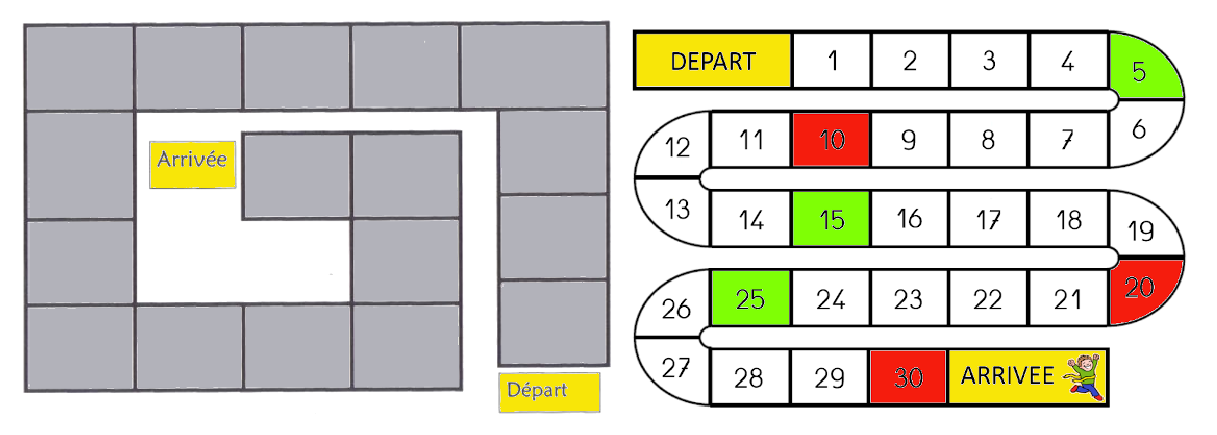
\includegraphics[width=16cm]{Nombres_et_calculs_did/Images/Num1_cours_jeux_de_l_oie}
   \end{center}  
   Selon {\it Claire Margolinas} (2005) [mar15], \og enseigner le nombre comme mémoire de la position demande de s'appuyer sur un milieu matériel qui comporte des files ayant une origine, une orientation et un rang, comme c'est le cas des objets de la figure 3. \fg
  \begin{center}
      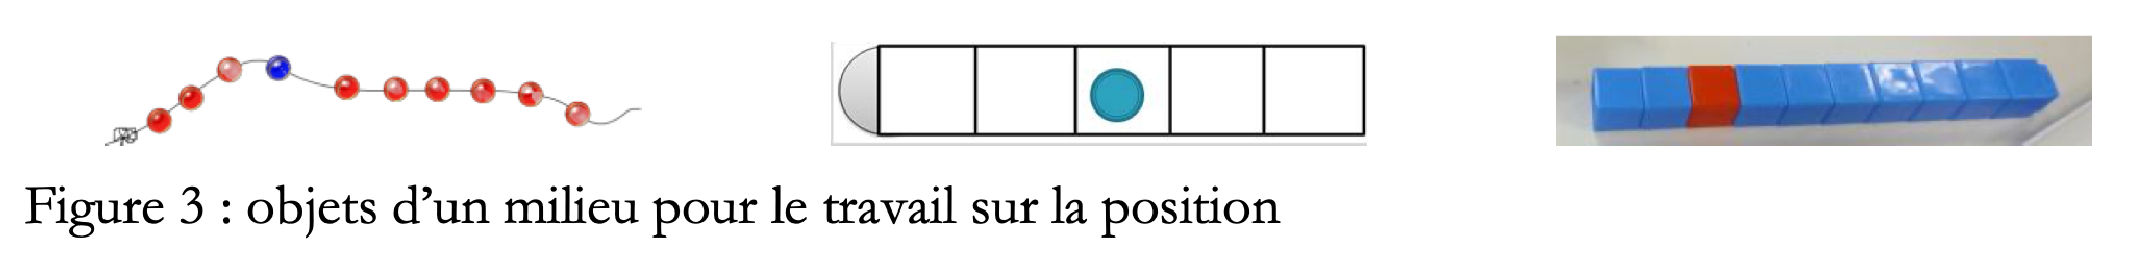
\includegraphics[width=16cm]{Nombres_et_calculs_did/Images/Num1_cours_Margolinas}
   \end{center}

\pagebreak
 
%%%%%%%%%%%%%%%%%%%%%%%%%%%%
\subsection{Construire les premiers savoirs et savoir-faire avec rigueur}

   {\bf Acquérir la suite orale des mots-nombres} : pour que cette suite soit disponible en tant que ressource pour dénombrer, il faut qu’elle soit stable, ordonnée, segmentée et suffisamment longue. La connaissance de la suite orale des noms des nombres ne constitue pas l’apprentissage du nombre mais y contribue.
Avant quatre ans, les premiers éléments de la suite numérique peuvent être mis en place jusqu’à cinq ou six puis progressivement étendus jusqu’à trente en fin de grande section. \\
   La comptine numérique peut être travaillée dans les activités rituelles telles que les comptines ou le comptage des présents/absents en GS, en n'oubliant pas de dire quel est le nombre total d'enfants présents ensuite. Enseigner la comptine numérique trop loin trop tôt est une activité qui n'a rien à voir avec une véritable construction du nombre : les élèves savent souvent \og compter \fg{} jusqu'à un certain nombre sans en comprendre le sens. \\
   
   {\bf Écriture des nombres avec les chiffres} : parallèlement, les enfants rencontrent les nombres écrits notamment dans des activités occasionnelles de la vie de la classe, dans des jeux et au travers d’un premier usage du calendrier. Les premières écritures des nombres sont introduites progressivement, à partir des besoins de communication au sein de la classe ou dans la résolution de problèmes concrets. L’apprentissage du tracé des chiffres se fait avec la même rigueur que celui des lettres, à partir de 4 ans.

   L'écriture en chiffres des nombres appartient à l'un des trois registres de représentation des nombres : le registre symbolique (les deux autres registres existants étant le registre analogique et le registre verbal).
   \begin{center}
      \begin{pspicture}(0,0)(12,8.25)
         \rput(5.5,7.5){\textcolor{B1}{\bf Registre analogique}}
         \psframe(3,5)(9,8)
         \rput(4,6){\psdice{4}}
         \rput(6,6.2){
\includegraphics[width=2cm]{Nombres_et_calculs_did/Images/Num1_cours_main4}}
         \pspolygon(7.5,5.2)(8,5.2)(8.3,5.5)(8.3,7.5)(7.8,7.5)(7.5,7.2)
         \psline(7.5,5.7)(8,5.7)(8.3,6)
         \psline(7.5,6.2)(8,6.2)(8.3,6.5)
         \psline(7.5,6.7)(8,6.7)(8.3,7)
         \psline(7.5,7.2)(8,7.2)(8.3,7.5)
         \psline(8,5.2)(8,7.2)
         \rput(2.5,2.5){\textcolor{B1}{\bf Registre symbolique}}
         \psframe(0,0)(5,3)
         \rput(1.25,1.25){\Huge 4}
         \rput(3.25,1.25){\includegraphics[width=1.8cm]{Nombres_et_calculs_did/Images/Num1_cours_chinois4}}
         \rput(9.5,2.5){\textcolor{B1}{\bf Registre verbal}}
         \psframe(7,0)(12,3)
         \rput(8.75,1.5){\Huge\cursive quatre}
         \rput(10.8,0.8){\Huge four}
        \psline[linewidth=1mm,linecolor=A1]{<->}(5.1,1.5)(6.9,1.5)
         \psline[linewidth=1mm,linecolor=A1]{<->}(2.5,3.1)(5,4.9)
         \psline[linewidth=1mm,linecolor=A1]{<->}(9.5,3.1)(7,4.9)
   \end{pspicture}
\end{center}

   Une grande attention doit être portée aux activités de dénombrement pour que soit évité le \og comptage-numérotage \fg. Elles doivent faire apparaître, lors de l’énumération de la collection, que chacun des noms de nombres désigne la quantité qui vient d’être formée. Les enfants doivent comprendre que toute quantité s’obtient en ajoutant un à la quantité précédente (ou en enlevant un à la quantité supérieure) et que sa dénomination s’obtient en avançant de un dans la suite des noms de nombres ou de leur écriture avec des chiffres. Pour dénombrer une collection d’objets, l’enfant doit être capable de synchroniser la récitation de la suite des mots-nombres avec le pointage des objets à dénombrer. Cette capacité doit être enseignée selon différentes modalités en faisant varier la nature des collections et leur organisation spatiale car les stratégies ne sont pas les mêmes selon que les objets sont déplaçables ou non, et selon leur disposition.
   
   Cette \og nouvelle \fg{} façon d'enseigner le nombre initiée par {\it Rémi Brissiaud} s'oppose à des théories plus anciennes mises en avant dans les années 1980 selon lesquelles le comptage devait précéder les activités de calcul, en référence aux cinq principes de deux chercheuses américaines, {\it Rochel Gelman} et {\it Charles Ransom Gallistel} :
{\renewcommand{\StringDOCUMENTATION}{Principes de Gelman}
\begin{documentation}
   \begin{enumerate}
      \item Le principe d’adéquation unique : chaque mot énoncé est mis en correspondance terme à terme avec un et un seul élément de la collection que l’on cherche à dénombrer.
      \item Le principe d’ordre stable : les mots utilisés doivent être toujours les mêmes et énoncés dans un ordre strict.
     \item Le principe cardinal : le dernier mot de la suite suffit pour exprimer la quantité.
      \item Le principe d’abstraction : on peut compter des objets disparates, quelle que soit la spécificité de chacun.
      \item le principe de non-pertinence de l’ordre : l’ordre dans lequel les éléments sont pris en compte est sans importance.
   \end{enumerate}
   \ \\ [-12mm]
\end{documentation}}


%%%%%%%%%%%%%%%%%%%%%%%%%%%%%%%%
\subsection{Des exemples de livres pour pratiquer\dots}

   Les premiers manuels de {\it Rémi Brissiaud} : \og J'apprends les maths \fg{} aux éditions Retz permettent une découverte des nombres et de leur utilisation très proches des attendus du programme : \\
   -- L'album 1 2 et 3 pour la PS ; \\
   -- Je compte\dots{} tu compares pour la MS/GS ; \\
   -- L'album à calculer pour la GS.

\begin{center}
   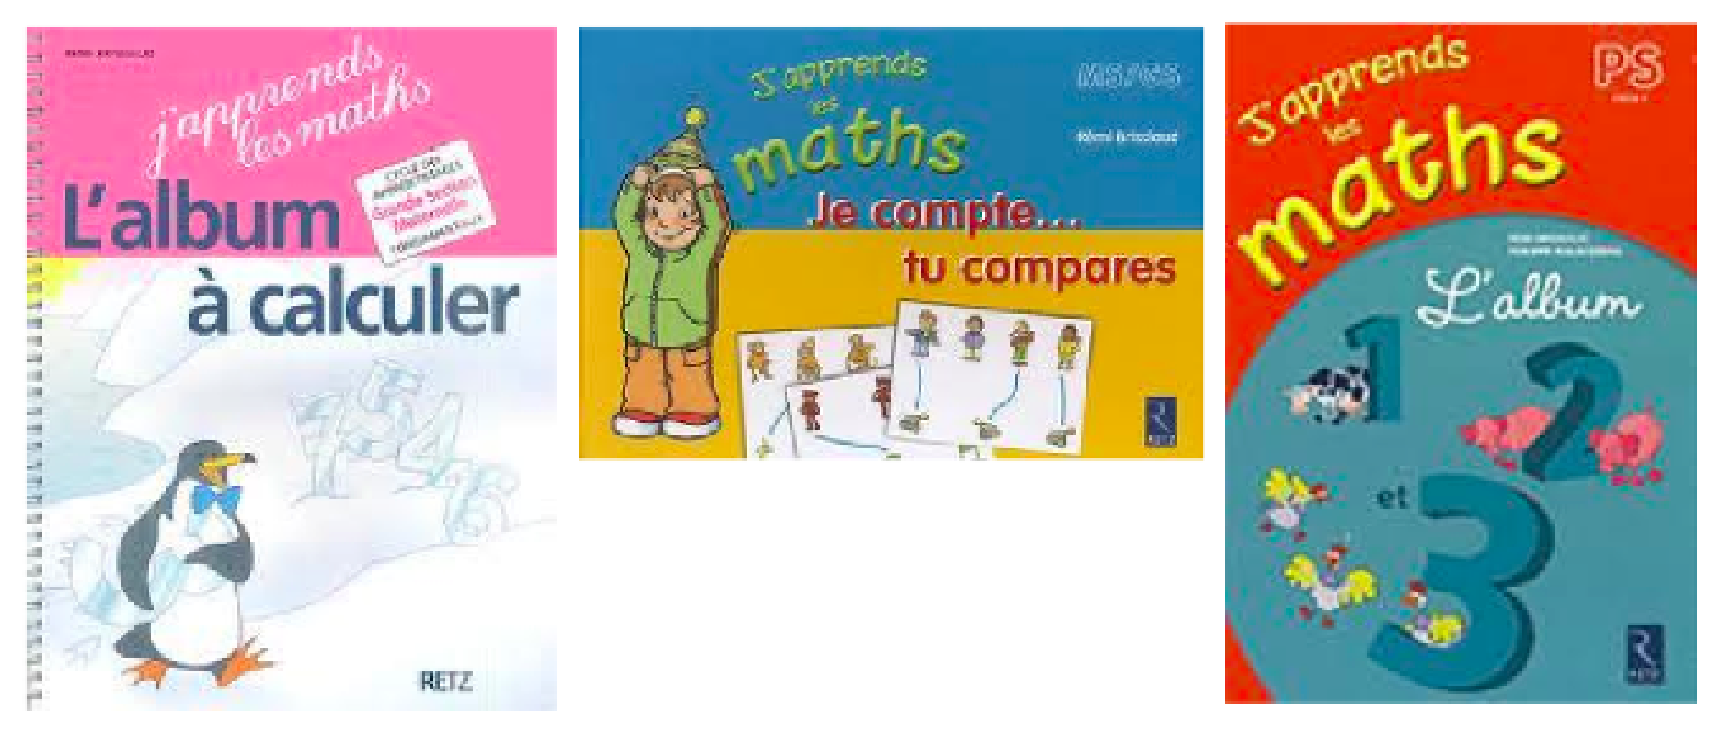
\includegraphics[width=17cm]{Nombres_et_calculs_did/Images/Num1_cours_livres}
\end{center}

Toute une série de livres inspirés de ces derniers existent pour des quantités et des thèmes différents. \\
Des exemples sont disponibles dans la partie \og Activités à faire en classe \fg.

\pagebreak


%%%%%%%%%%%%%%%%%%%%%%%%%%%%%%%%
\section{Construction de notre numération positionnelle de base 10}

   D'après les repères annuels de progression, au CP, les élèves poursuivent le travail mené à la maternelle sur les nombres inférieurs à 10. En période 2, ils réalisent des groupements par 10 et s'exercent à échanger 10 unités pour une dizaine et inversement. Le travail de groupements par 10 permet d’aborder rapidement les nombres supérieurs à 20 (jusqu’à 60 au moins) pour travailler sur les aspects positionnel et décimal de la numération écrite. La désignation orale des nombres est démarrée en période 3 : \og 53, c’est 5 dizaines et 3 unités ; c’est (5 fois 10) et (3 fois 1) \fg. Les nombres jusqu’à 100 sont introduits suffisamment tôt (en période 4 au plus tard) pour pouvoir être maîtrisés à la fin du CP. \\ 
   Au CE1, les élèves poursuivent l’étude de la numération décimale en travaillant avec des centaines. La connaissance des nombres jusqu’à 100 est consolidée, notamment pour leur désignation orale et pour le calcul mental. Ils apprennent à multiplier par 10 pour mieux construire mentalement la numération décimale. \\
   En CE2, les élèves poursuivent l’étude de la numération décimale en travaillant avec des milliers. Parallèlement, la connaissance des nombres jusqu’à 1 000 est consolidée, notamment pour leur désignation orale et pour le calcul mental. Ils renforcent leur connaissance de la multiplication par 10 et apprennent à multiplier par 100. \\
   En CM1, les élèves apprennent à utiliser et à représenter les grands nombres entiers jusqu’au million. Il s'agit d'abord de consolider les connaissances (écritures, représentations\dots). \\
   En CM2, le répertoire est étendu jusqu’au milliard. \\

{\bf Codage des nombre entiers} : imaginons une grande quantité d'objets à dénombrer, le comptage un par un serait long et fastidieux. Différentes étapes vont permettre aux élèves de dénombrer cette quantité et de la coder, c'est notamment le but de l'activité \og \href{https://www.google.com/url?sa=t&rct=j&q=&esrc=s&source=web&cd=&ved=2ahUKEwie2PjG_vfrAhVFXBoKHfOTCpIQFjAFegQIBBAB&url=http%3A%2F%2Fwww.ac-grenoble.fr%2Fiennyons%2Fneosite%2FIMG%2Fpdf%2Fles_fourmillions.pdf%3F2505%2F6a472f235b620f5480ccb061ffd10470aacf5863&usg=AOvVaw345EqweQSy_91yxab-XCEr}{Les fourmillons} \fg{}, de la collection {\it Ermel}.
\begin{center}
\renewcommand{\arraystretch}{2.2}
\begin{Ltableau}{0.95\linewidth}{3}{c}
   \hline
   Étape & Représentation & Explications \\
   \hline
   état initial
   &
   {\psset{unit=0.6}
   \begin{pspicture}(0,-0.2)(10,3)
      \multips(0,0){46}{\pscircle[fillstyle=solid,fillcolor=A1](! rand 1000 mod 100 div rand 250 mod 100 div){.15}}
\end{pspicture}}
   &
   quantité d'objets (jetons, pois, allumettes\dots{}) à dénombrer \\
   \hline
   groupements
   &
   {\psset{unit=0.6}
   \begin{pspicture}(-5.3,-1)(5,1)
      \psset{fillstyle=solid,fillcolor=A1}
      \rput(-5,0){\Dix}
      \rput(-2.75,0){\Dix}
      \rput(-0.5,0){\Dix}
      \rput(1.75,0){\Dix}
      \rput(4,0){\Cinq}
     \pscircle(4.75,0){.12}
   \end{pspicture}}
   &
   groupements par 10, éventuellement sous la forme de constellations \\
   \hline
   échanges
   &
   {\psset{unit=0.6}
   \begin{pspicture}(-5.3,-1)(5,1.25)
      \psset{fillstyle=solid,fillcolor=A1}
      \rput(-5,0){\psframe(-.4,-.4)(1.2,.4)}
      \rput(-2.75,0){\psframe(-.4,-.4)(1.2,.4)}
      \rput(-0.5,0){\psframe(-.4,-.4)(1.2,.4)}
      \rput(1.75,0){\psframe(-.4,-.4)(1.2,.4)}
      \rput(4,0){\Cinq}
     \pscircle(4.75,0){.12}
   \end{pspicture}}
   &
   échange de chaque paquet de 10 par une enveloppe de valeur 10 \\
   \hline
   codage visuel
   &
   {\psset{unit=0.6cm}
   \begin{pspicture}(-2,-0.5)(2,1.5)
      \psline[linewidth=.8pt,](0,-0.5)(0,1.3)
      \rput(-1.2,1){\textcolor{A1}{d}}
      \rput(1.2,1){\textcolor{A1}{u}}
      \psset{fillstyle=solid,fillcolor=A1}
      \pscircle(-1,-.2){.12}
      \pscircle(-1,.2){.12}
      \pscircle(-1.4,.2){.12}
      \pscircle(-1.4,-.2){.12}
      \rput(1,0){\Cinq \pscircle(0,0){.12}\pscircle(.5,0){.12}}
   \end{pspicture}}
   &
   représentation des dizaines et unités par le même objet, qui a donc une valeur différente suivant sa position \\
   \hline
   codage chiffré
   &
   {\psset{unit=0.6cm}
   \begin{pspicture}(-2,-0.5)(2,1.5)
      \psline[linewidth=.8pt,](0,-0.5)(0,1.3)
      \rput(-1.2,1){\textcolor{A1}{d}}
      \rput(1.2,1){\textcolor{A1}{u}}
      \rput(-1.2,0){\Huge 4}
      \rput(1.2,0){\Huge 6}
   \end{pspicture}}
   &
   codage de la quantité dans notre système positionnel de numération de base 10 \\
   \hline
\end{Ltableau}
\end{center}

\pagebreak

On peut résumer les étapes d'apprentissages par la frise suivante : 

\begin{center}
\begin{pspicture}(0.8,0)(16,3.2)
   \pspolygon[linewidth=1pt,linearc=.25,framearc=0,linecolor=A1!20,fillstyle=solid,fillcolor=A2!20](0,0)(3,0)(4,1.5)(3,3)(0,3)(1,1.5)
   \rput(2,2.3){CP}
   \rput(2,0.7){{\Large$\to$} 100}
   \rput(3.05,0){\pspolygon[linewidth=1pt,linearc=.25,framearc=0,linecolor=A1!40,fillstyle=solid,fillcolor=A2!40](0,0)(3,0)(4,1.5)(3,3)(0,3)(1,1.5)
   \rput(2,2.3){CE1}
   \rput(2,0.7){{\Large$\to$} 1\,000}}
   \rput(6.10,0){\pspolygon[linewidth=1pt,linearc=.25,framearc=0,linecolor=A1!60,fillstyle=solid,fillcolor=A2!60](0,0)(3,0)(4,1.5)(3,3)(0,3)(1,1.5)
   \rput(2,2.3){CE2}
   \rput(2,0.7){{\Large$\to$} 10\,000}}
   \rput(9.15,0){\pspolygon[linewidth=1pt,linearc=.25,framearc=0,linecolor=B1!40,fillstyle=solid,fillcolor=B2!40](0,0)(3,0)(4,1.5)(3,3)(0,3)(1,1.5)
   \rput(2,2.3){CM1}
   \rput(2,0.7){{\Large$\to$} 1\,000\,000}}
   \rput(12.20,0){\pspolygon[linewidth=1pt,linearc=.25,framearc=0,linecolor=B1!60,fillstyle=solid,fillcolor=B2!60](0,0)(3,0)(4,1.5)(3,3)(0,3)(1,1.5)
   \rput(2,2.3){CM2}
   \rput(2,0.7){{\Large$\to$} 1\,000\,000\,000}}
   \psline[arrowlength=2,linewidth=1mm]{->}(0.9,1.5)(16.7,1.5)
\end{pspicture}
\end{center}


%%%%%%%%%%%%%%%%%%%%%%%%%%%%%%
\section{Les irrégularités de notre comptine orale} %%%%%
%%%%%%%%%%%%%%%%%%%%%%%%%%%%%%

\textbf{Les irrégularités dans les noms des nombres de 0 à 100} [dav18] : la compréhension de notre système de numération reste difficile au CP et au CE1, et pour cause : même s'il est préconisé d'étudier les nombres jusqu'à 100 au CP, les irrégularités sont nombreuses dans cette tranche : 

{\small
\begin{pspicture}(-1,-3)(18,11.3)
   \psframe[fillstyle=solid,fillcolor=lightgray!50,linecolor=lightgray!50](-0.9,0.4)(9.6,10.6)
   \multido{\iColonne=0+1}{10}{\rput[Br](\iColonne,10){\iColonne}}
   \multido{\iColonne=0+1}{10}{\multido{\iBLigne=9+ -1,\iLigne=1+1}{9}{\rput[Br](\iColonne,\iBLigne){\iLigne\iColonne}}}
   \psframe[linewidth=1.5pt,linecolor=blue,framearc=0.75](-.7,.6)(.3,8.6)
   \psframe[linewidth=1.5pt,linecolor=red,framearc=0.75](.3,8.8)(6.3,9.4)
   \psframe[linewidth=1.5pt,linecolor=violet,framearc=0.5](-0.6,8.7)(9.4,10.5) 
   \psframe[linewidth=1.5pt,linecolor=violet,framearc=0.5](9.4,2.7)(-0.6,4.5) 
   \psframe[linewidth=1.5pt,linecolor=violet,framearc=0.5](-0.6,0.7)(9.4,2.5)
   \psset{arrowscale=2,arrows=->}
   \rput(6.25,9.3){\rnode{a}{}}
   \rput(10.3,9.5){\rnode{b}{}}
   \rput(13.3,8){{\begin{minipage}{5cm}
      Premières irrégularités venant très tôt dans la numération : onze, douze, treize, quatorze, quinze et seize sont des nouveaux mots-nombres qui sont les contractés des expressions latines correspondantes pour lesquelles l'unité précède la dizaine ({\it tredecim} signifie \mbox{$3+10$}). Dans une numération régulière, ces nombres se diraient \og dix-un, dix-deux, dix-trois, dix-quatre, dix-cinq et dix-six \fg{}.
   \end{minipage}}}
   \ncline[linecolor=red]{a}{b}
   \rput(9.2,8.8){\rnode{f}{}}
   \rput(9.4,3.6){\rnode{c}{}}
   \rput(9.4,1.6){\rnode{d}{}}
   \rput(13.3,3){\rnode{e}{\begin{minipage}{4cm}
      Présence de blocs de nombres \og exprimés \fg{} en base vingt.
   \end{minipage}}}
   \ncline[linecolor=violet]{c}{e}
   \ncline[linecolor=violet]{d}{e}
   \ncline[linecolor=violet]{f}{e}
   \rput(0,.6){\rnode{f}{}}
   \rput(5.5,-1.5){\rnode{g}{\begin{minipage}{12cm}
      Concernant les dizaines, de nouveaux mots-nombres apparaissent : vingt, trente, quarante...{} Dans une numération régulière, ces nombres s'exprimeraient ainsi : \og deux-dix, trois-dix, quatre-dix... \fg. Puis, plus loin,  les nombres soixante-dix, quatre-vingts et quatre-vingt-dix pourraient être qualifiés de nombres \og doublement irréguliers \fg{} : les mots français \og septante, octante et nonante \fg{} subsistent en Suisse et en Belgique, mais plus en France, depuis le 19\ieme~siècle. \end{minipage}}}
   \ncline[linecolor=blue]{f}{g}
\end{pspicture}}


On s'aperçoit ainsi que la numération orale est une source de difficulté importante pour la compréhension de notre numération parce qu’elle n’est pas en adéquation avec la numération écrite. Plus globalement, on peut résumer les principales différences dans le tableau suivant :

\vspace{0.3cm}
{\small
\renewcommand{\arraystretch}{1.5}
\begin{tabular}{|C{1.5}||C{3.5}|C{3.4}||C{3.4}|C{3.3}|}
   \hline
   \cellcolor{FondTableaux}{} & \multicolumn{2}{c||}{\cellcolor{FondTableaux}{Désignation orale des nombres}} & \multicolumn{2}{c|}{\cellcolor{FondTableaux}{Désignation écrite des nombres}} \\
   \hline
   Éléments de la numération & 26 mots jusqu'au milliard, plus la conjonction \og et\fg\
   &
   zéro, un, deux, trois, quatre, cinq, six, sept, huit, neuf, dix, onze, douze, treize, quatorze, quinze, seize, vingt, trente, quarante, cinquante, soixante, cent, mille, million, milliard, et
   &
   10 signes appelés chiffres (indo-arabes)
   &
   0, 1, 2, 3, 4, 5, 6, 7, 8, 9 \\
   \hline
   Statut du zéro
   &
   absent si on considère uniquement l'écriture des nombres entiers naturels
   &
   deux-cent-cinq \newline \newline trois-millions
   &
   nécessaire pour une meilleure visibilité, justifié par le caractère positionnel de notre numération pour marquer le \og manque \fg{} d'un ordre
   &
   205 \newline \newline
   3\,000\,000 \\
   \hline
   Structure
   &
   additive si le nombre est constitué de deux mots-nombres en ordre décroissant, multiplicative s'il est constitué de deux mots-nombres en ordre croissant, mixte par combinaison des deux propriétés précédentes
   &
   vingt-quatre, \newline c'est $20+4$ \newline \newline quatre-vingts, \newline c'est $4\times20$ \newline \newline quatre-vingt-douze, \newline c'est $4\times20+12$
   &
   stable, justifiée par notre numération positionnelle de base 10
   &
   234 \newline \newline=~$2\times100$ + \mbox{$3\times10$} + $4\times1$ \newline \newline$=2\times10^2$ +\mbox{$3\times10^1$} + $4\times10^0$ \\
   \hline
   Ordre des éléments
   &
   succession de mots qui n'a pas toujours de sens, selon une permutation des mots réglée par une grammaire
   &
   cent-quarante-trois \newline \cancel{cent-trois-quarante} \newline \cancel{quarante-cent-trois} \newline \cancel{quarante-trois-cent} \newline trois-cent-quarante \newline \cancel{trois-quarante-cent}
   &
   succession de chiffres toujours possible (mais de sens différent) & 345, 354, 435, 453, 534, 543 \\
   \hline
\end{tabular}}

\section{L'écriture des nombres}

{\small Les règles d'orthographe françaises sont réputées difficiles, celles de l'écriture des nombres n'échappent pas à la règle ;-)}
{\renewcommand{\StringDOCUMENTATION}{Règles orthographiques conformes à la réforme de 1990}
\begin{documentation}
\begin{itemize}
   \item Les numéraux composés sont systématiquement reliés par des traits d’union : deux-millions-cent-mille-trente-et-un ; trente-et-unième.
   \item Les mots [vingt] et [cent] prennent un -s lorsqu'il y en a plusieurs et qu'ils se trouvent à la fin du nombre : mille-deux-cent-trente, trente-mille-cent, mille-trois-cents.
   \item Les mots qui indiquent les classes [mille], [million], [milliard] prennent un -s quand il en a plusieurs, sauf [mille] qui est invariable : un-milliard-deux-cent-millions-trois-mille-cent. \\ [-8mm]
\end{itemize}
\end{documentation}}


%%%%%%%%%%%%%%%%%%%%%%%%%%%%%%%%
\section{Des outils pour la numération} %%%%%%
%%%%%%%%%%%%%%%%%%%%%%%%%%%%%%%

La capacité grouper-échanger peut être travaillée en classe avec différents matériels. Les matériels dessinés sur les fiches de travail doivent correspondre à des matériels réels que les élèves peuvent manipuler puis progressivement s'en passer. Il existe différentes sortes de matériels pédagogiques (liste non exhaustive !). 
\begin{center}
{\renewcommand{\arraystretch}{1.5}
\begin{Ltableau}{\linewidth}{2}{C{11}|C{5}}
   \hline
   Objets & Visuel \\
   \hline
   \begin{minipage}{10cm}
      Les \textbf{boites de picbille}, (Rémi Brissiaud) permettent de travailler les groupements par 5 et par 10 , l'échange 10 contre 1, les compléments à 5 et à 10, les notions de dizaines et d'unité.
   \end{minipage}
   &
   \begin{minipage}{5cm}  
      \ \\ [3mm]
      
\includegraphics[width=5cm]{Nombres_et_calculs_did/Images/Num1_cours_boite_picbille}
      \ \\
   \end{minipage} \\
   \hline
   \begin{minipage}{10cm}
      Le matériel \textbf{multibase}, emboîtable ou non, sous forme de \textbf{cubes} unités, de \textbf{barres} de 10, de \textbf{plaques} de 100 et de gros \textbf{cubes} de 1\,000 permet de visualiser les groupements.
   \end{minipage}
   &
   \begin{minipage}{5cm}
      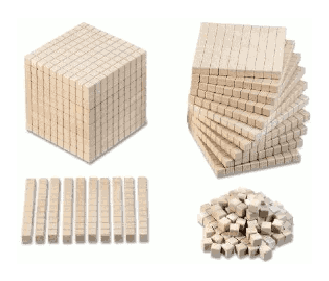
\includegraphics[width=4.5cm]{Nombres_et_calculs_did/Images/Num1_cours_multibase}
   \end{minipage} \\
   \hline
   \begin{minipage}{10cm}
      Le \textbf{boulier numérateur}, ou boulier européen, à utiliser tel quel (une boule = une unité) pour se créer une image mentale des dizaines (une rangée) et des unités (une boule). La lecture des nombres de fait en fonction du nombre de rangées entières activées et du nombre de boules seules.
   \end{minipage}
   & 
   \begin{minipage}{5cm}
      \quad 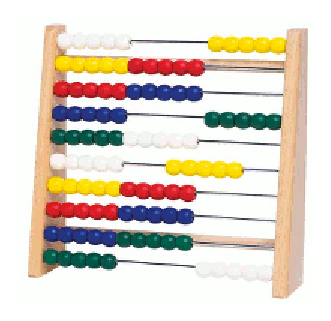
\includegraphics[width=4.5cm]{Nombres_et_calculs_did/Images/Num1_cours_boulier_num}
   \end{minipage} \\
   \hline
   \begin{minipage}{10cm}
      Le \textbf{boulier chinois} (par exemple) utilise sur chaque tige des boules valant une unité de l'ordre considéré, les unaires (en dessous) et des boules valant cinq unité de l'ordre considéré, les quinaires (au dessus). Les nombres se codent comme dans notre numération, les unités étant placées à droite.
   \end{minipage}
   &
   \begin{minipage}{5cm}
      \ \\ [1mm]
      \quad 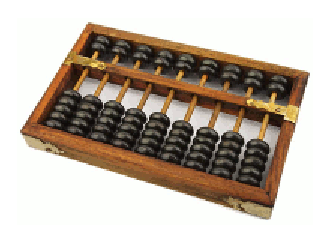
\includegraphics[width=4.5cm]{Nombres_et_calculs_did/Images/Num1_cours_boulier_chinois}
   \end{minipage} \\
   \hline
   \begin{minipage}{10cm}
      Les \textbf{abaques} (à jetons, romain) à construire avec les élèves ou à photocopier, il en existe de différentes sortes (avec ou sans quinaire, avec quadrillage horizontal ou vertical), on peut les utiliser avec des jetons de type haricots, pois\dots
   \end{minipage}
   &
   \begin{minipage}{5cm}
      \ \\ [1mm]
      \qquad \includegraphics[width=3.5cm]{Nombres_et_calculs_did/Images/Num1_cours_abaque_jetons} \\ [-2mm]
   \end{minipage} \\
   \hline
\end{Ltableau}}
\end{center}


%%%%%%%%%%%%%%%%%%%%%%%%%%%%%
%%%%%%%%%%%%%%%%%%%%%%%%%%%%%
\activites

\textcolor{G1}{Sujet n°3 de l'épreuve de leçon, concours CRPE 2022, académie de Montpellier.} \\

{\bf\uline{Consigne candidat}} : À partir du sujet et du dossier proposés par le jury, vous concevrez la mise en œuvre d'une séance d'enseignement à l'école primaire dans chacune des deux disciplines français et mathématiques. Vous présenterez successivement les composantes pédagogiques et didactiques de chaque séance et son déroulement. \\

{\bf\uline{Sujet}} : Construire le nombre pour exprimer des quantités. \\

{\bf\uline{Contexte de la séance d'enseignement}} : \\
   \hspace*{5mm} -- cycle d'enseignement : cycle 1 ; \\
   \hspace*{5mm} -- niveau de la classe : GS ; \\
   \hspace*{5mm} -- positionnement de la séance de mathématiques : \\
      \hspace*{10mm} -- période : période 5; \\
      \hspace*{10mm} -- séquence dans laquelle elle s'insère : découvrir les nombres et leurs utilisations. \\ [5mm]

{\bf\uline{Documents fournis au candidat}} : \\

{\bf\uline{Document 1}} : Bulletin officiel n°25 du 24 juin 2021, extrait du programme d'enseignement de l'école maternelle. 

\begin{center}
   \fbox{
      \begin{minipage}{15cm}
         \textsf{{\bf 4.1. Découvrir les nombres et leurs utilisations} \\ [1mm]
         Depuis leur naissance, les enfants ont une intuition des grandeurs qui leur permet de comparer et d'évaluer de manière approximative les longueurs (les tailles), les volumes, mais aussi les collections d'objets divers (\og il y en a beaucoup ! \fg, \og pas beaucoup \fg, etc.). {\bf À leur arrivée à l'école maternelle}, ils commencent à discriminer les petites quantités, un, deux et parfois trois. Enfin, s'ils savent énoncer les débuts de la suite numérique, cette récitation ne traduit pas une véritable compréhension des quantités et des nombres. \\ [3mm]
         L'école maternelle doit conduire progressivement chacun à comprendre que les nombres permettent à la fois d'exprimer des quantités (usage cardinal) et d'exprimer un rang ou une position dans une liste (usage ordinal). Cet apprentissage demande du temps et la confrontation à de nombreuses situations impliquant des activités pré-numériques puis numériques. Il nécessite un enseignement structuré, {\bf pendant toute la durée du cycle1}, afin qu'à l'issue de l'école maternelle les connaissances et compétences acquises forment un socle solide sur lequel appuyer les apprentissages ultérieurs.}
      \end{minipage}
   }
\end{center}

\bigskip


{\bf\uline{Document 2}} : Note de service n°2019-085 du 28 mai 2019, Recommandations pédagogiques, apprentissage fondamental à l'école maternelle . Découvrir les nombres et leurs utilisations. \\

\begin{center}
   \begin{minipage}{15cm}
      \begin{flushleft}
         \textsf{{\bf UN APPRENTISSAGE PROGRESSIF, QUI S'APPUIE SUR LE LANGAGE ORAL ET ÉCRIT} \\ [3mm]
         La découverte du nombre et de ses utilisations est liée à la construction d'un langage oral et écrit précis qui contribue à structurer les connaissances et à les fixer en mémoire. La verbalisation par I'enseignant et par l'élève des actions réalisées et de leurs résultats constitue une aide importante à la prise de conscience des procédures utilisées et de leurs effets. L'enseignant est attentif à organiser les échanges oraux pour aider à structurer les apprentissages des élèves : il aide à décrire les situations, les relations, à Justifier et commence à argumenter ; il attire I'attention sur certaines procédures et connaissances utilisées en situation ; il Introduit le vocabulaire spécifique (noms des nombres, adverbes de quantité) pour que les enfants se l'approfondissent et l'utilisent.}
      \end{flushleft}
   \end{minipage}
\end{center}

\begin{center}
   \begin{minipage}{15cm}
      \begin{flushleft}
         \textsf{L'usage des chiffres est une partie Importante de la découverte du nombre. Il soutient l'élaboration de sa représentation mentale. Les premières écritures chiffrées des nombres sont Introduites progressivement en lien avec I'appropriation de la quantité correspondante et la résolution de situations concrètes. En ajoutant une contrainte d'éloignement dans l'espace et dans le temps dans I'organisation d'une situation, ou en demandant de transmettre une information sans parler, on rend nécessaire l'utilisation d'une trace écrite pour garder des Informations en mémoire. Cet usage de l'écrit pour se souvenir est une découverte importante. L'enseignant aide à comprendre que la conservation de l'information de quantité passe par I'élaboration d'un code commun (les nombres) et mobilise rapidement cette connaissance.}
      \end{flushleft}
   \end{minipage}
\end{center}
  
\bigskip

{\bf\uline{Document 3}} : J.P Blanc, P. Bramand, A. Vargas, D. Peynichou, E. Lafont, C.Maurin, N. Blanc, {\it Pour comprendre les mathématiques GS}, Hachette éducation, juillet 2015, page 68.

\begin{center}
   \fbox{\includegraphics[width=12cm]{Nombres_et_calculs_did/Images/Num1_CRPE_chapeau}}
\end{center}


%%%%%%%%%%%%%%%%%%%%%%%%%%%%%
%%%%%%%%%%%%%%%%%%%%%%%%%%%%%
\analyses


\begin{exercice}[Étude de productions d'élèves]
Les exercices et productions d'élèves proposés sont tirés de l'ouvrage \og Variations sur une leçon de mathématiques \fg, paru aux éditions {\it L'Harmattan}, sous la direction de {\it C. Blanchard-Laville.} \\ [1mm]
Les exercices suivants ont été proposés au tableau dans une classe de CM1 au mois d'octobre :
\begin{center}
\fbox{\textsl{
\begin{minipage}{15cm}
   \begin{enumerate}
      \item Écrire en chiffres le nombre deux-millions-trois-cent-quarante-mille-cent-cinq. 
      \item Écrire en chiffres le nombre dix-sept-millions-deux-mille-cinquante-huit.
   \end{enumerate}
\end{minipage}}}
\end{center}

L'exercice 1 est corrigé collectivement avant que l'exercice 2 ne soit donné aux élèves. Dans les séances précédentes, les élèves ont travaillé l'écriture des grands nombres, ce qui a conduit à l'introduction, pour faciliter la lecture, d'un espace entre les classes qui correspondent à des tranches de trois chiffres, et l'enseignant a conclu : \og On remplace les mots millions et mille par des espaces\fg. \\
Voici les productions relevées pour chacun des exercices :
\begin{center}
\begin{ltableau}{0.7\linewidth}{4}
   \hline
   \multicolumn{2}{|c|}{Exercice 1} & \multicolumn{2}{c|}{Exercice 2} \\
   \hline
   2 340 105 & 17 élèves & 17 002 058 & 11 élèves \\
   2 340 500 & 6 élèves & 17 200 058 & 5 élèves \\
   2 340 050 & 1 élève & 17 200 58 & 2 élèves \\
   200003004015015 & 1 élève & 17 2 058 & 1 élève \\
   234500 & 1 élève & 17 2000 058 & 1 élève \\
   & & 17 2000 58 &1 élève \\
   & & 17 2 58 & 5 élèves \\
   \hline
\end{ltableau}
\end{center}
\begin{enumerate}
   \item Expliquez la différence de réussite entre les deux exercices. 
   \item Faites une hypothèse d'interprétation des réponses dans le premier exercice :
   \begin{enumerate}
      \item pour la réponse 2 340 500  ;
      \item pour la réponse 200003004015015. 
   \end{enumerate}
   \item Dans l'exercice 2, pour chacune des réponses 17 200 058 et 17 2 58, indiquez en quoi elle respecte ou non les conventions usuelles d'écriture et la conclusion du maître. 
   \item Quel argument devrait permettre aux élèves de rejeter la réponse 17 200 058 ? \\
   Permet-il de rejeter 17 2 58 ? Pourquoi ? 
   \item Proposez un nombre qui pourrait poser problème aux adeptes de la réponse 17 2 58 et les inciter à repérer les inconvénients de leur proposition. Justifiez votre réponse. 
\end{enumerate}
\end{exercice}

\begin{corrige}
\ \\ [-5mm]
\begin{enumerate}
   \item L'exercice 1 est réussi à 65\,\% et le deuxième à 42\,\%. Il est plus difficile de placer les chiffres 0 dans l'écriture du second nombre que dans celui du premier : à l'oral, on entend distinctement les nombres qui constituent les tranches de trois chiffres pour le premier nombre, mais pas pour le second où il faut juxtaposer des 0 en début de tranche afin que cette tranche contienne trois chiffres.
   \item 
   \begin{enumerate}
      \item Les élèves ont probablement inversé mentalement les termes [cent] et [cinq]. Ceux-ci apparaissant en fin de nombre, ils étaient peut-être moins concentrés et en surcharge cognitive.
      \item Le système de  numération ne semble pas complètement acquis. En effet, il écrit les nombres \og comme il les entend \fg{} : deux millions (qu'il écrit 20000 en omettant deux chiffres 0), trois cent (qu'il écrit correctement 300), quarante (qu'il écrit correctement 40), mille cent cinq (qu'il n'écrit pas correctement du tout, mais qu'il écrit tout de même avec les chiffres 0, 1 et 5 entendus ou pressentis dans la désignation orale).
   \end{enumerate}
   \item Pour 17 200 058, l'écriture respecte la convention usuelle d'écriture par tranches de trois chiffres. Mais, par contre, il est à noter une erreur de position des chiffres dans la seconde tranche (200 au lieu de 002), ce qui ne respecte pas la convention usuelle d'écriture d'un nombre. La convention du maître n'est pas respectée car sinon, on aurait lu \og deux-cent-mille \fg{} et non \og deux-mille \fg{} comme dans l'énoncé. \\
   Pour 17 2 58, l'élève ne respecte pas la convention usuelle d'écriture par tranches de trois chiffres. Par contre, la convention du maître est respectée scrupuleusement : les mots [millions] et [mille] sont remplacés par des espaces.
   \item Pour rejeter la réponse 17 200 058, une simple re-lecture du nombre devrait permettre de se rendre compte que l'oralisation du \og deux-cent \fg{} ne devrait pas paraître. Cet argument ne devrait pas permettre de rejeter la réponse 17 2 58, pour des élèves qui vont donner au premier espace le sens de million et pour le second le sens de mille.
   \item Tout nombre se lisant sans le mot-nombre [mille] : par exemple \og douze-millions-quatorze \fg{}, l'élève pourra écrire 12 14 et s'apercevoir qu'il manque au moins la tranche des mille.
\end{enumerate}
\end{corrige}

\bigskip

\begin{exercice}[Étude d'un exercice]
\begin{minipage}{6cm}
   Cet exercice est extrait de \textit{Cap maths CP}, éditions {\it Hatier}.
   En faire une analyse a priori : 
   \begin{enumerate}
      \item compétences mises en jeu ;
      \item procédures utilisables par l'élève ;
      \item erreurs prévisibles.
   \end{enumerate}
\end{minipage}
\qquad
\fbox{
\begin{minipage}{10cm}
   Relie chaque nombre à la case qui lui correspond. \\
   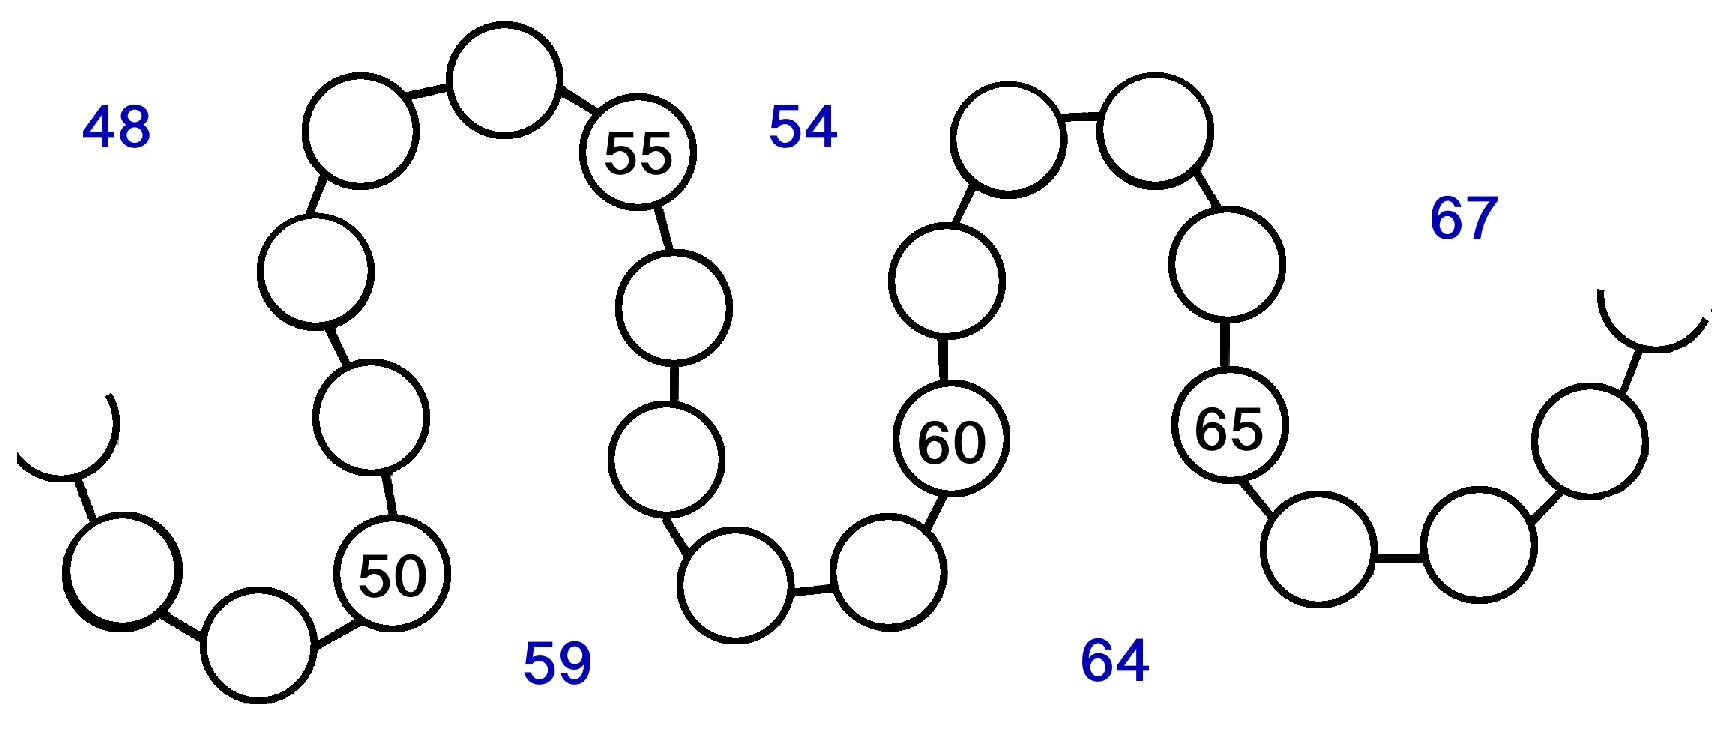
\includegraphics[width=10cm]{Nombres_et_calculs_did/Images/Num1_analyse_perles}
\end{minipage}}
\end{exercice}

\begin{corrige}
\ \\ [-5mm]
\begin{enumerate}
   \item Compétences mises en jeu : être capable d'écrire, ranger les nombres entiers naturels inférieurs à 100 et avoir compris l'organisation, l'aspect algorithmique de notre numération positionnelle de base 10.
   \item Procédures utilisables par l'élève, par exemple :
   \begin{itemize}
      \item l'élève peut placer dans les cases tous les nombres manquants, et ensuite relier chaque nombre à la case représentant le même nombre ;
      \item il peut également réciter \og mentalement \fg{} la comptine numérique en indiquant à chaque fois le case correspondante, et placer au fur et à mesure les nombres qu'ils récite ;
      \item il peut utiliser les compléments à 5 ou à 10 et avancer ou reculer par rapport à une case déjà remplie (par exemple 59, c'est $60-1$, donc une case avant la case 60\dots).
   \end{itemize}
   \item Erreurs prévisibles, par exemple :
   \begin{itemize}
      \item le nombre 48 peut ne pas avoir été placé, car l'élève compte à partir de 50 ;
      \item les nombres peuvent être associés à une case située \og entre \fg{} deux nombres déjà placés (par exemple 64 entre 60 et 65), sans lien avec le nombre de cases ;
      \item l'élève peut avoir placé par exemple 59 juste après 55, c'est à dire dans l'ordre (de plus petit au plus grand), sans se soucier la suite des nombres de 1 en 1 ;
      \item il a pu associer à chaque nombre la case marquée \og la plus proche \fg{} (par exemple, relier 54 à 55).
   \end{itemize}   
\end{enumerate}
\end{corrige}

\clearpage

%\begin{exercice}[CRPE 2014 G1]
%   Un enseignant propose un jeu de bataille à ses élèves de maternelle. Il utilise un jeu de cartes représentant les nombres de 1 à 6. Voici douze cartes extraites du jeu : par exemple, la première carte (en haut à gauche) représente le nombre 3 et la dernière carte (en bas à droite) représente le nombre 5.
%   \begin{center}
%      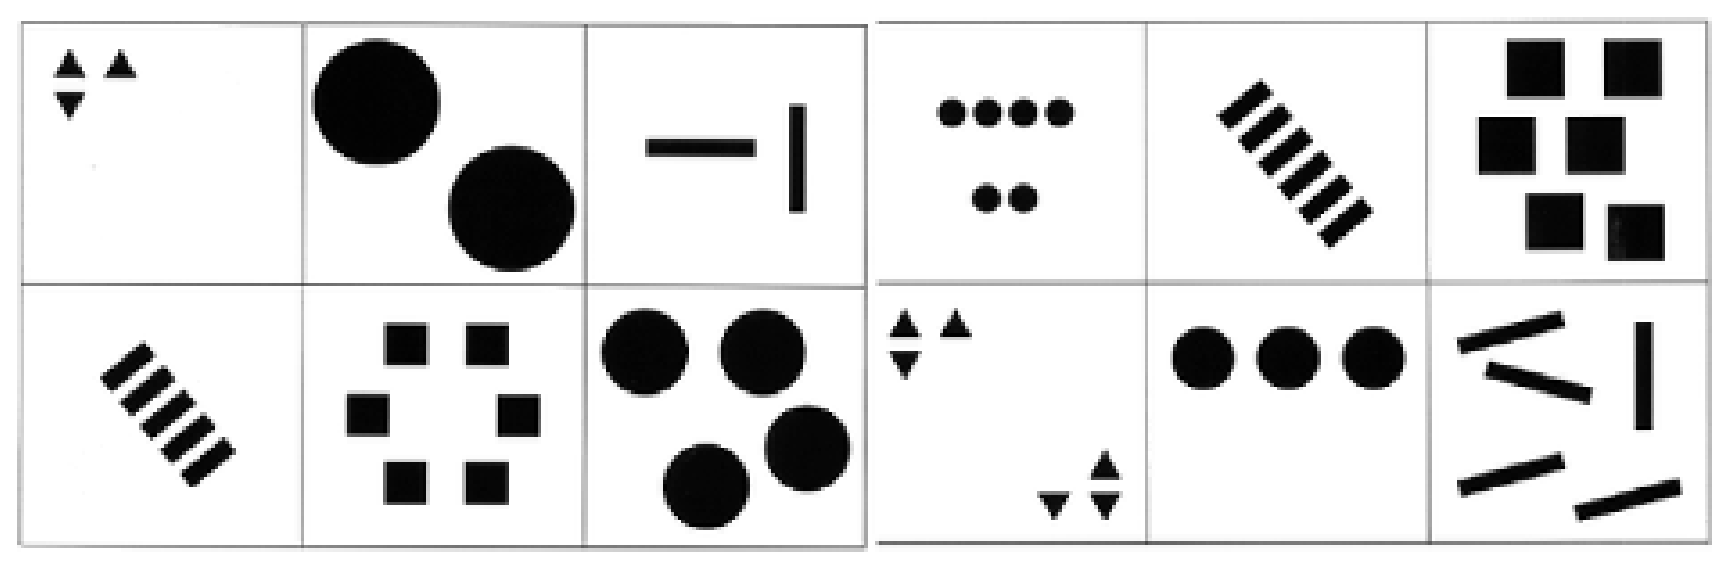
\includegraphics[width=12cm]{Nombres_et_calculs_did/Images/Num1_analyse_bataille1} \\
%      {\it \og Vers les maths, Maternelle moyenne section \fg{} p.130 et 131, Édition ACCES, 2009.}
%   \end{center}
%   Voici la règle du jeu :
%   \begin{center}
%   \fbox{\begin{minipage}{15cm}
%      Deux élèves s'opposent. Les cartes sont battues puis distribuées, puis chacun des deux élèves pose ses cartes, à l'envers, en tas devant lui. \\
%      Ils retournent chacun une carte : celui dont la carte représente le nombre le plus grand remporte les deux cartes et les met sous son tas. \\
%      En cas d'égalité, chaque élève retourne une nouvelle carte sur la table. Celui dont la nouvelle carte représente le nombre le plus grand remporte toutes les cartes retournées sur la table. \\
%      À la fin, celui qui n'a plus de carte a perdu. \\
%      {\it (On peut aussi arrêter le jeu au bout d'un certain temps et compter les cartes de chacun des deux élèves : celui qui a le plus de cartes a gagné).}
%   \end{minipage}}
%   \end{center}
%   \begin{enumerate}
%      \item Citer deux compétences mathématiques travaillées par les élèves lors de ce jeu de bataille.
%      \item Pour chaque compétence citée en réponse à la question 1), donner deux causes possibles d'erreurs.
%      \item L'enseignant peut utiliser un autre jeu de cartes représenté ci-dessous : \\
%      \begin{center}
%         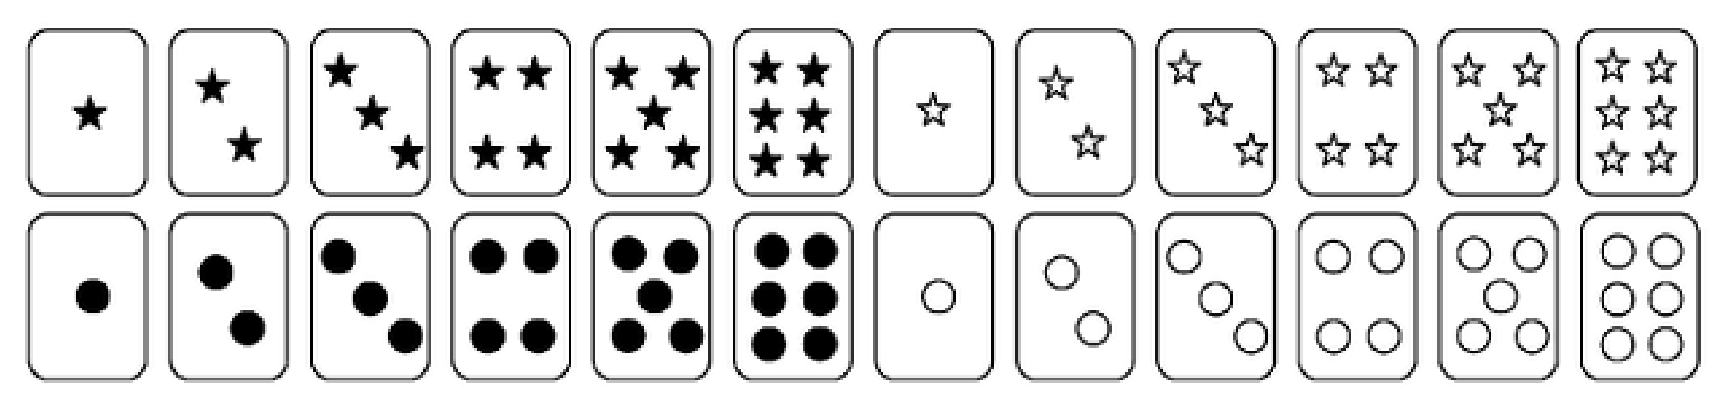
\includegraphics[width=16cm]{Nombres_et_calculs_did/Images/Num1_analyse_bataille2}
%      \end{center}
%      \bigskip
%      Comparer les intérêts respectifs de chacun des jeux au regard des deux compétences citées en réponse à la question 1.
%   \end{enumerate}
%\end{exercice}
%
%\begin{corrige}
%\ \\ [-5mm]
%\begin{enumerate}
%   \item On peut choisir par exemple deux compétences parmi les trois compétences suivantes qui font appel à une procédure numérique ou non numérique (a) et b), ou a) et c)). \\
%   \begin{enumerate}
%      \item Comparer deux collections en utilisant le nombre d'éléments de ces collections : procédure numérique, éventuellement par perception globale.
%      \item Comparer deux collections en utilisant la correspondance terme à terme : procédure non numérique.
%      \item Comparer deux collections par perception visuelle, que l'on considère comme procédure non numérique si on ne fait que comparer sans dénombrer.
%   \end{enumerate}
%   \item Causes possibles d'erreurs pour chaque compétence. \\
%   \begin{enumerate}
%      \item Par dénombrement :
%      \begin{itemize}
%         \item la non stabilité de la comptine : l'élève dit par exemple \og un, deux, quatre\fg ; \\
%         \item la non acquisition du principe cardinal : l'élève associe bien chaque élément de la comptine à un objet, mais ne sait lequel de ces mots-nombres représente à lui seul le cardinal de la collection ;
%        \item l'élève compte plusieurs fois le même élément de la carte, ou en oublie.
%     \end{itemize}
%     \item Par correspondance terme à terme, les sources d'erreurs peuvent provenir :
%     \begin{itemize}
%        \item des dispositions différentes des constellations ;
%        \item des différences de formes et de taille des objets ;
%        \item du fait qu'il faille effectuer cette correspondance terme à terme mentalement.
%     \end{itemize}
%     \item Par perception visuelle, les sources d'erreurs peuvent provenir :
%     \begin{itemize}
%        \item des dispositions différentes des constellations ;
%        \item de la taille et de la forme des objets qui font que certaines collections prennent \og plus de place \fg{} que d'autres.
%   \end{itemize}
%   \end{enumerate}
%   \item Globalement, le jeu 1 est plus difficile que le jeu 2, donc son avantage principal réside dans le fait qu'il emmènera les élèves à réfléchir à des stratégies efficaces de comparaison. Le jeu 2 étant plus simple par la présence des constellations, il peut être avantageux pour une première approche du jeu ou comme élément de différentiation. \\ [3mm]
%   \qquad
%   {\renewcommand{\arraystretch}{1.5}
%   \begin{CLtableau}{0.85\linewidth}{3}{c}
%      \hline
%      & Intérêt du jeu 1 & Jeu Intérêt du jeu 2 \\
%      \hline
%      a)
%      &
%      dénombrement par perception visuelle difficile en raison des constellations non standard, ce qui incite l'élève à dénombrer un à un et à utiliser le principe cardinal.
%      &
%      dénombrement direct en raison des constellations classiques, procédure simple et à encourager lorsque la situation le permet. \\
%      \hline
%      b)
%      &
%      vraie correspondance terme à terme, dans le sens celle-ci n'est pas instinctive : l'élève doit trouver le moyen d'effectuer cette correspondance mentalement.
%      &
%      la disposition en constellations facilite la comparaison : on voit facilement, par exemple; que la constellation 5 c'est celle du 4 plus quelque chose. \\
%      \hline
%      c)
%      &
%      présence de leurres perceptifs : les objets sont différents par leur forme et leur taille, ce qui implique une concentration accrue lors de la comparaison.
%      &
%      comparaison directe en raison des constellations identiques dans leur forme standard. \\
%      \hline
%   \end{CLtableau}}
%\end{enumerate}
%\end{corrige}
%
%\bigskip

\begin{exercice}[CRPE 2016 G1]
Un enseignant de moyenne section de maternelle utilise le jeu ci-dessous avec ses élèves.
\begin{center}
   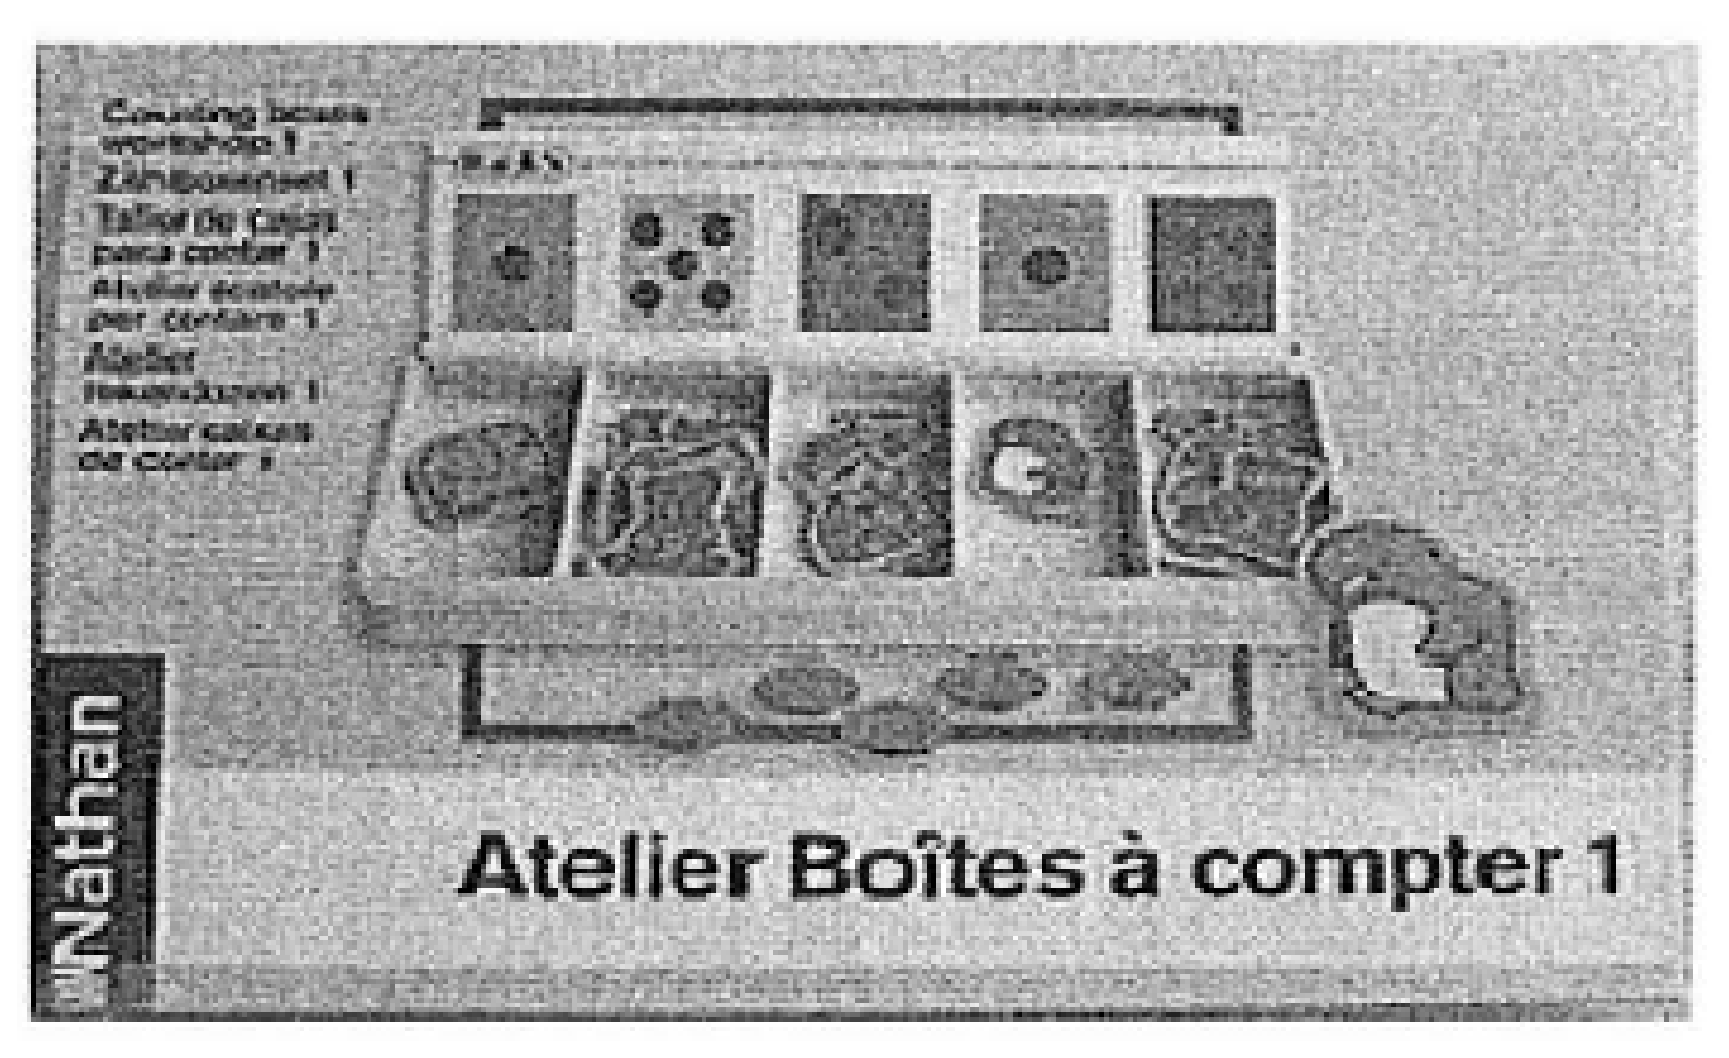
\includegraphics[width=10cm]{Nombres_et_calculs_did/Images/Num1_analyse_boite1} \\
   {\it Atelier Boites à compter 1, Nathan, 2003}
\end{center}
La boite contient le matériel suivant :
\begin{center}
   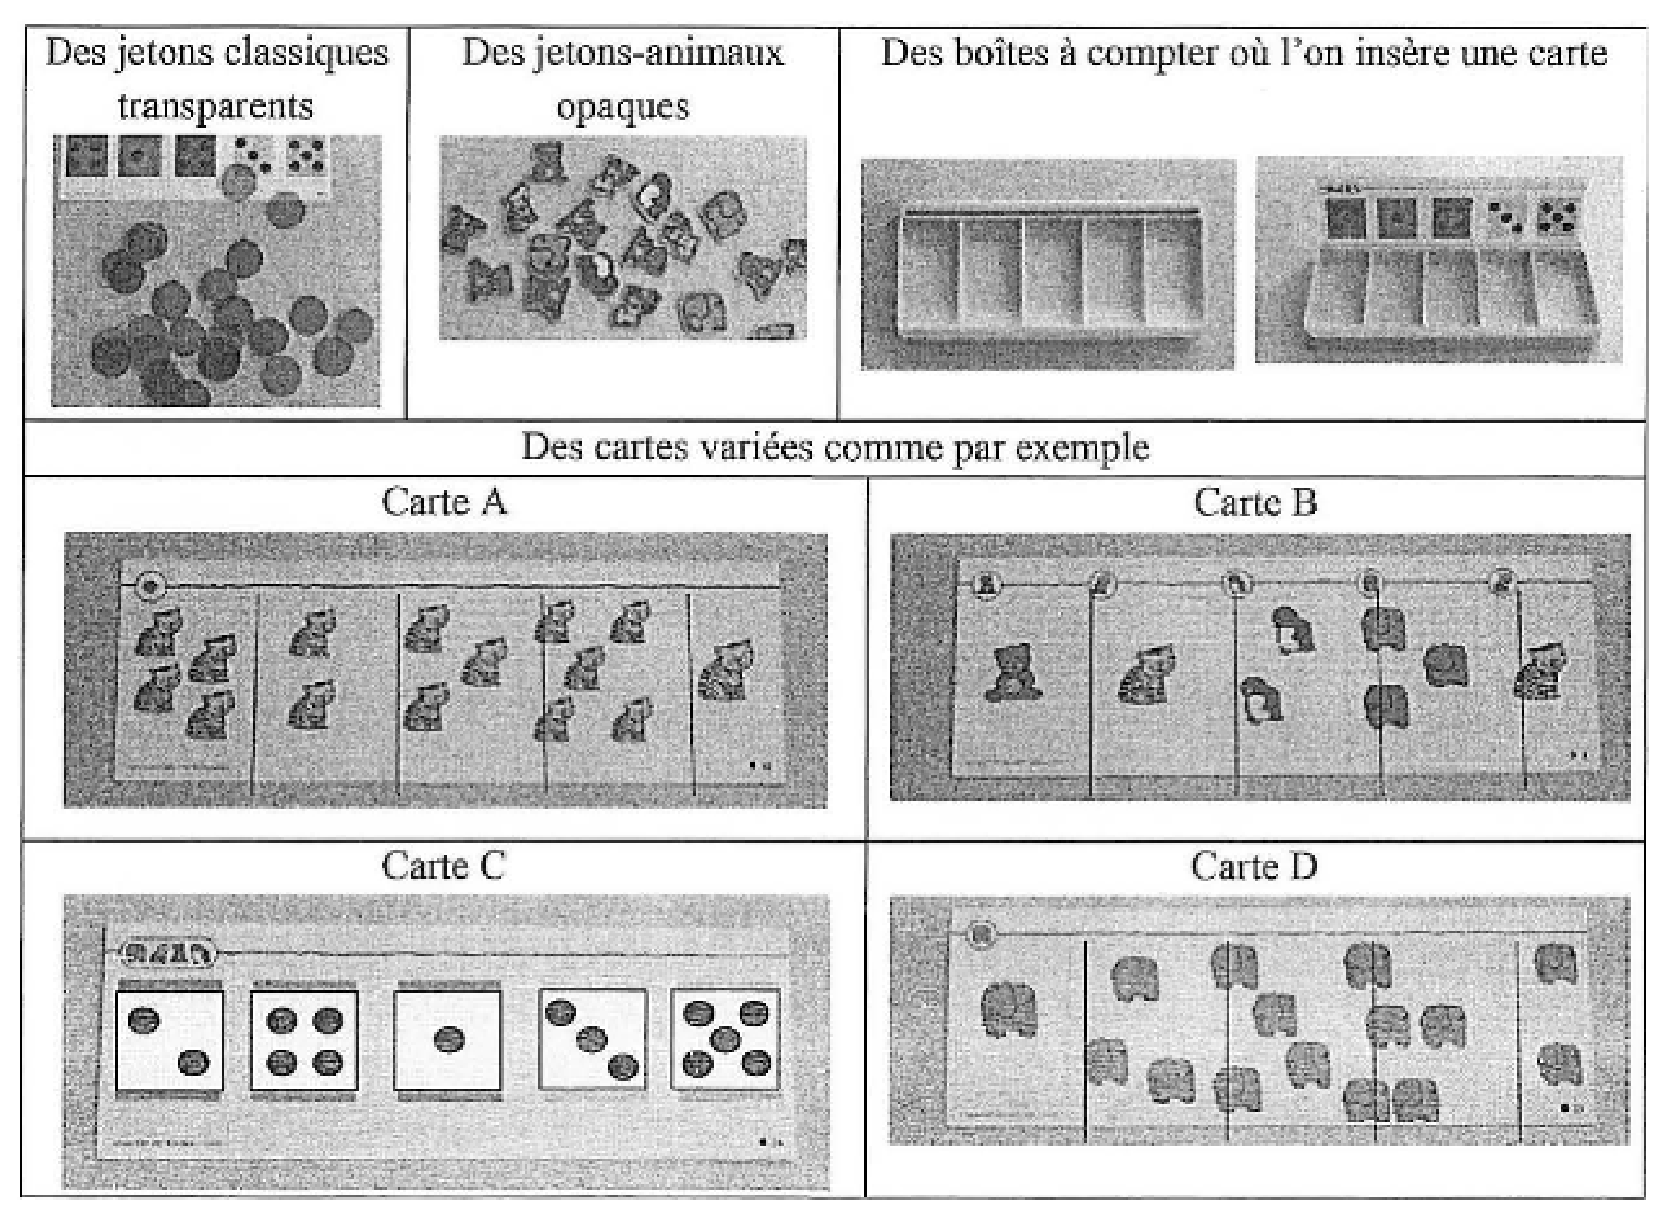
\includegraphics[width=16cm]{Nombres_et_calculs_did/Images/Num1_analyse_boite2} \\ [3mm]
   \fbox{\begin{minipage}{16cm}
   Pour chaque élève, l'enseignant choisit une carte et des jetons (animaux ou classiques). \\
   L'objectif du maître est de faire réaliser par l'élève des collections de jetons de cardinaux identiques à ceux de la carte.
\end{minipage}}
\end{center}
\begin{enumerate}
   \item 
   \begin{enumerate}
      \item Analyse a priori. Pour chacune des deux configurations matérielles ci-dessous : \\
      $\bullet$ donner deux méthodes que pourraient utiliser les élèves pour dénombrer les collections proposées. \\
      $\bullet$ donner deux erreurs que les élèves sont susceptibles de faire en réalisant les collections.
      \smallskip
      \begin{center}
          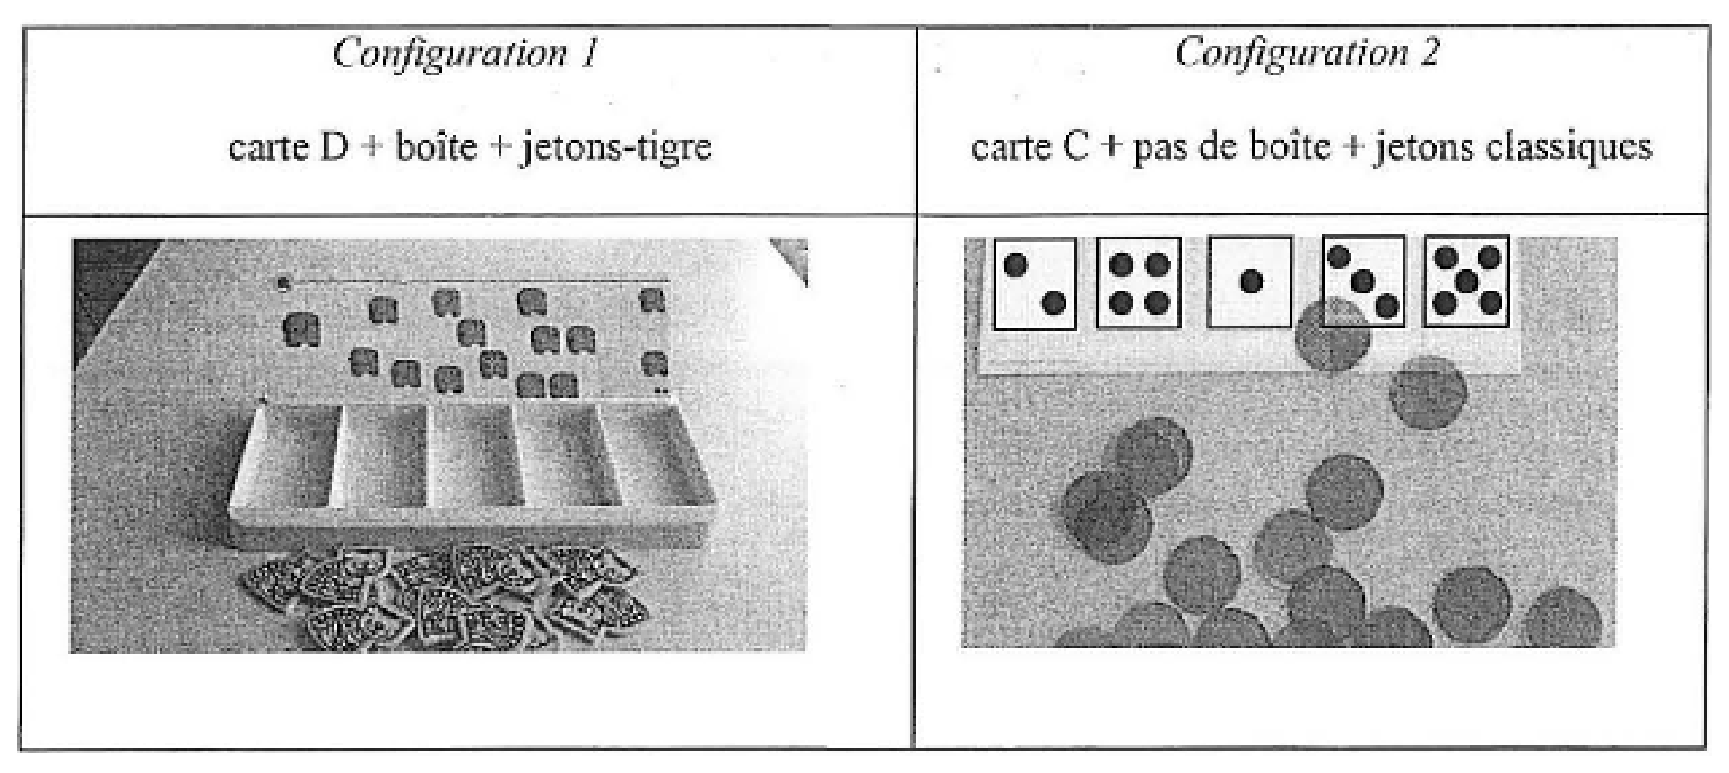
\includegraphics[width=16cm]{Nombres_et_calculs_did/Images/Num1_analyse_boite3}
      \end{center}   
      \item Voici ci-dessous deux réalisations d'élèves pour la configuration 2. \\   
      Que semblent-ils avoir compris tous les deux ? Analyser les différences éventuelles.
      \smallskip
      \begin{center}
         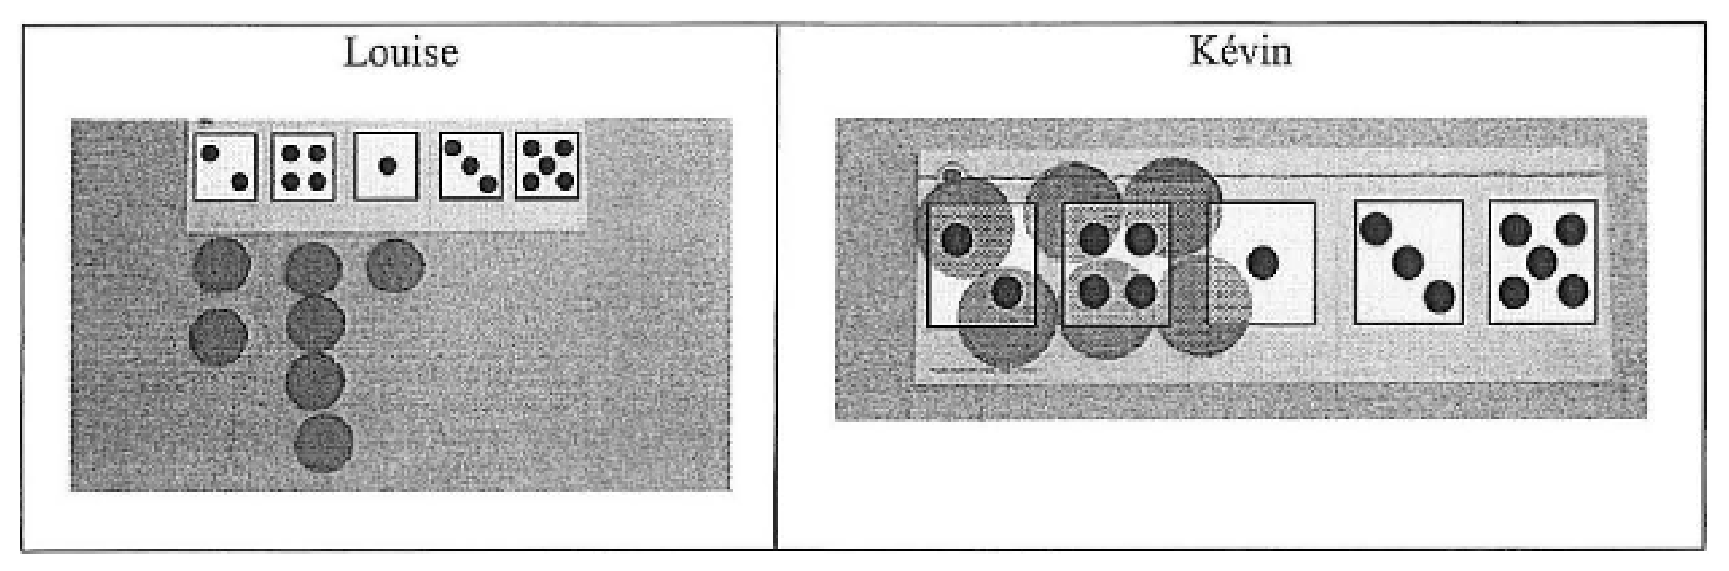
\includegraphics[width=16cm]{Nombres_et_calculs_did/Images/Num1_analyse_boite4}
      \end{center}
    \end{enumerate}
    \item Voici une autre production d'élève en réponse à une autre configuration matérielle.
    \smallskip
    \begin{center}
      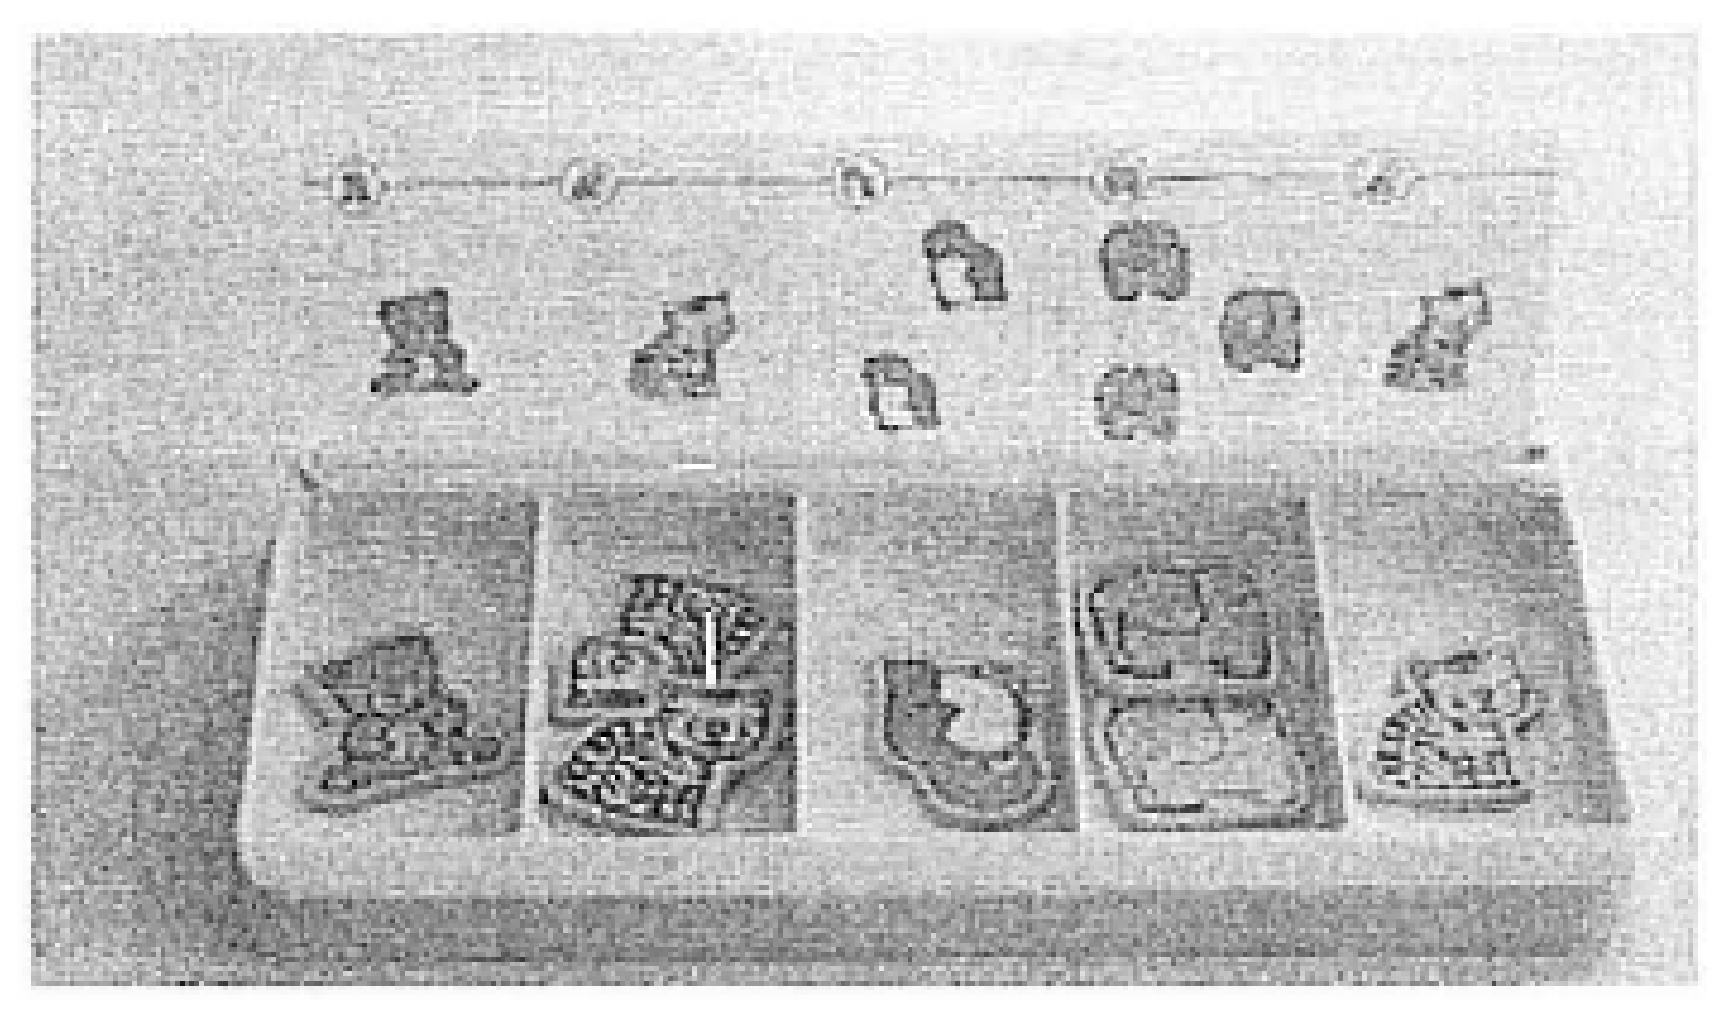
\includegraphics[width=9cm]{Nombres_et_calculs_did/Images/Num1_analyse_boite5}
   \end{center}       
   Citer une facilité et une difficulté qu'apporte le choix d'une configuration matérielle incluant une boîte.
\end{enumerate}
\end{exercice}

\begin{corrige}
\ \\ [-5mm]
\begin{enumerate}
   \item
   \begin{enumerate}
      \item Les méthodes (M1 et M2) et les erreurs (E1 et E2) sont récapitulées dans le tableau ci-dessous : \\ [1mm]   
         {\renewcommand{\arraystretch}{1.5}
         \begin{CLtableau}{1\linewidth}{3}{c}
             \hline
             &
             Configuration 1
             &
             Configuration 2 \\
             \hline
             M1
             &
             \multicolumn{2}{c|}{\bf Procédure par subitisation (reconnaissance perceptive immédiate d'une quantité)} \\
             &
             Procédure possible pour des petites quantités (nombres inférieurs à 5). Ici, l'élève \og voit \fg{} un certain nombre d'éléphants.
             &
             Pour la carte C, cette procédure devrait être immédiate car les nombres sont représentés sous forme de configurations géométriques particulières : celles des constellations du dé, qui sont une des représentations des nombres vues dès la PS. \\
             \hline
             M2
             &
             \multicolumn{2}{c|}{\bf Procédure par comptage un à un.} \\
             &
             \multicolumn{2}{p{14cm}|}{Utilisation de la comptine numérique : suite de mots-nombre mis en correspondance un à un avec les éléments de la collection considérée, le dernier mot-nombre utilisé indiquant la quantité (principe cardinal).} \\
             \hline
             E1
             &
             Procédure par subitisation : l'élève peut se tromper dans la reconnaissance des quantités, surtout si celles-ci dépassent 3.
             &
             Erreur liée au matériel : le fait de ne pas avoir de boite ne favorise pas le rangement des jetons, l'élève va disposer ses jetons sous sa carte, mais certains jetons peuvent se mélanger avec la représentation du nombre précédent.
             \\
             \hline
             E2
             &
             \multicolumn{2}{c|}{\bf Erreurs de comptage.} \\
             &
             \multicolumn{2}{p{14cm}|}{$\bullet$ L'élève dénombre deux fois le même objet ou il en oublie un (principe d'adéquation unique). \newline
             $\bullet$ L'élève se trompe dans l'ordre de la comptine numérique (principe d'ordre stable).} \\
             \hline
          \end{CLtableau}}
       \bigskip
       \item Louise et Kévin ont compris l'objectif du maître, à savoir de réaliser des collections de cardinaux identiques à ceux de la carte. Cependant, leurs procédures semblent différentes :
       \begin{itemize}
          \item Louise dispose ses jetons les uns en dessous des autres. On peut imaginer qu'elle a tout d'abord dénombré les jetons de la carte (par subitisation ou comptage), puis qu'elle a réalisé une collection de jetons de même cardinal en les plaçant un à un.
          \item Kévin semble procéder par correspondance terme à terme en posant un jeton sur chaque point du dé. Cette procédure n'utilise pas le dénombrement mais est tout à fait efficiente, même si, avec des jetons beaucoup plus gros que les points de la carte, l'organisation matérielle pourra poser problème pour les deux dernières constellations (3 et 5).
       \end{itemize}     
    \end{enumerate}
    \item
    \begin{itemize}
       \item Une facilité : les jetons représentant les animaux sont bien rangés en regard de la collection de la carte témoin, ne dépassent pas et donc ne se mélangeront pas.
       \item Une difficulté : il sera difficile pour l'élève de vérifier son résultat pour des quantités supérieures à deux puisqu'alors les jetons vont se recouvrir ou se chevaucher.
    \end{itemize}
 \end{enumerate}
\end{corrige}

\bigskip


\begin{exercice}[CRPE 2017 G1]
Dans une classe de maternelle, une enseignante donne à un groupe d’élèves la consigne suivante :
\begin{center}
\fbox{
\begin{minipage}{15cm}
   \og J’ai installé trois poupées avec leur assiette autour de cette table pour le goûter. Elles pourront commencer leur goûter quand il y aura un biscuit dans l’assiette de la poupée blonde, un biscuit dans l’assiette de la poupée brune et un biscuit dans l’assiette de la poupée rousse. \\
   Les biscuits du goûter se trouvent dans une boîte dans le coin cuisine. \\
   Vous devez aller chercher juste ce qu’il faut de biscuits pour le goûter des poupées. Vous pouvez faire plusieurs voyages. \fg
\end{minipage}
}
\end{center}
La table des poupées est éloignée de quelques mètres du coin cuisine. \\
L’information suivante \og la boîte contient 5 biscuits \fg{} n’est pas donnée aux élèves. \\
On appelle \og voyage \fg{} un aller au coin cuisine et un retour à la table des poupées.
\begin{itemize}
   \item L’élève A a effectué 3 voyages, rapportant un seul biscuit à chaque fois.
   \item L’élève B a effectué 1 voyage. Il utilise sa main droite dont il abaisse deux doigts. Il se déplace à la table du coin cuisine et revient avec 3 biscuits dans la main gauche.
   \item L’élève C effectue très rapidement 1 voyage. Il a pris 3 biscuits.
   \item L’élève D effectue 2 voyages. Au premier voyage il ramène tous les biscuits. Au deuxième il rapporte 2 biscuits à la cuisine.
\end{itemize}
\vspace*{-5mm}
\begin{enumerate}
   \item Quel aspect du nombre est mobilisé dans cette situation ?
   \item Analyser les stratégies mises en oeuvre par chacun des élèves.
   \item Proposer une modification interne à l’énoncé de la situation susceptible d’engager les élèves A et D à évoluer dans la construction du nombre. Expliciter cette évolution.
\end{enumerate}
\end{exercice}

\begin{corrige}
\ \\ [-5mm]
\begin{enumerate}
   \item C'est l'aspect cardinal du nombre qui est ici mobilisé (construire le nombre pour exprimer les quantités) : en effet, l'élève doit comprendre qu'un objet est une unité, en dehors de toute considération de forme, d'utilité, puis construire le principe cardinal, c'est à dire concevoir que le dernier mot-nombre de la liste ayant servi à énumérer désigne, à lui seul, le nombre total d'éléments de la collection. \\
   À ce titre, l'objectif pour l'élève est de ramener autant de biscuits qu'il y a de poupées ou d'assiettes.
   \bigskip
   \item On remarque tout d'abord que tous les élèves ont rempli le contrat et sont arrivés au résultat escompté, mais avec des procédures différentes.
   \begin{itemize}
      \item L'\textbf{élève A} va chercher les biscuits un à un, jusqu'à ce qu'il ait rempli toutes les assiettes. On ne peut pas affirmer qu'il ait dénombré les assiettes ou les biscuits, mais plutôt qu'il a fait une \og correspondance terme à terme \fg{} entre les assiettes et les biscuits.
      \item L'\textbf{élève B} a dénombré les assiettes, ce qu'il modélise par des doigts levés : il est probable qu'il ait effectué une correspondance terme à terme entre les assiettes et les doigts, ou qu'il ait compté en même temps qu'il levait ses doigts un à un. Il effectue probablement la même procédure pour déterminer le nombre de biscuits à rapporter.
      \item L'\textbf{élève C} est probablement l'élève ayant le mieux compris le principe cardinal : il a entendu ou/et vu qu'il y avait 3 assiettes (par subitisation ou dénombrement), il ramène donc 3 biscuits, il n'a pas besoin à ce stade d'aide particulière (doigts, correspondance\dots{}). 
      \item L'\textbf{élève D} ramène tous les biscuits de la cuisine, il distribue les biscuits en en mettant un par assiette, puis il ramène les biscuits \og en trop \fg{}. \\ 
   \end{itemize}
   \bigskip
   \item Pour les élèves A et D, on peut observer qu'ils utilisent une méthode de \og remplissage \fg{} des assiettes sans utiliser les caractéristiques des nombres. Il effectuent tous les deux plusieurs voyages pour arriver au bon résultat. \\
   Pour qu'ils engagent une procédure inhérente à la construction du nombre, on pourrait préciser dans l'énoncé que seul un voyage est autorisé. Ils devront alors réfléchir à la manière de ramener 3 biscuits \og du premier coup \fg.
\end{enumerate}
\end{corrige}

\bigskip


\begin{exercice}[CRPE 2018 G2]
Voici un extrait du programme de l’école maternelle publié dans le bulletin officiel n\degre2 du 26 mars 2015.
\begin{center}
\fbox{
\begin{minipage}{15cm}
   La stabilisation de la notion de quantité, par exemple trois, est la capacité à donner, montrer, évaluer ou prendre un, deux ou trois et à composer et décomposer deux et trois. Entre deux et quatre ans, stabiliser la connaissance des petits nombres (jusqu’à cinq) demande des activités nombreuses et variées portant sur la décomposition et recomposition des petites quantités [\dots], la reconnaissance et l’observation des constellations du dé, la reconnaissance et l’expression d’une quantité avec les doigts de la main, la correspondance terme à terme avec une collection de cardinal connu. [\dots] Après quatre ans, les activités de décomposition et recomposition s’exercent sur les quantités jusqu’à dix.
\end{minipage}}
\end{center}
\begin{enumerate}
   \item Citer deux procédures qu’un élève de fin de petite section peut utiliser pour affirmer qu’une collection est constituée de trois objets.
   \item Proposer une activité à mettre en place en moyenne section pour travailler les décompositions du nombre quatre.
   \item Un enseignant de grande section décide d’utiliser avec ses élèves un dé dont les faces sont représentées ci-dessous. Quel intérêt peut-il y avoir à utiliser un tel dé ?
   \begin{center}
   {\psset{unit=0.4}
   \begin{pspicture}(0,-0)(38.5,5.5)
      \rput(0,0){\psframe(0,0)(6,5) \pscircle(1.5,3.5){0.5}} 
      \rput(6.5,0){\psframe(0,0)(6,5) \pscircle(1.5,3.5){0.5} \pscircle(1.5,1.5){0.5}}
      \rput(13,0){\psframe(0,0)(6,5) \pscircle(1.5,3.5){0.5} \pscircle(1.5,1.5){0.5} \pscircle(3,3.5){0.5}}
      \rput(19.5,0){\psframe(0,0)(6,5) \pscircle(1.5,3.5){0.5} \pscircle(1.5,1.5){0.5} \pscircle(3,3.5){0.5} \pscircle(3,1.5){0.5}}
      \rput(26,0){\psframe(0,0)(6,5) \pscircle(1.5,3.5){0.5} \pscircle(1.5,1.5){0.5} \pscircle(3,3.5){0.5} \pscircle(3,1.5){0.5} \pscircle(4.5,3.5){0.5}}
      \rput(32.5,0){\psframe(0,0)(6,5) \pscircle(1.5,3.5){0.5} \pscircle(1.5,1.5){0.5} \pscircle(3,3.5){0.5} \pscircle(3,1.5){0.5} \pscircle(4.5,3.5){0.5} \pscircle(4.5,1.5){0.5}}
   \end{pspicture}}
   \end{center}
\end{enumerate}
\end{exercice}

\begin{corrige}
\ \\ [-5mm]
\begin{enumerate}
   \item Un élève peut utiliser les procédures suivantes :
   \begin{itemize}
      \item correspondance terme à terme avec une autre collection constituée de trois objets ;
      \item perception visuelle globale de trois objets (ou subitisation) ;
      \item comptage-dénombrement de la quantité : un et un (deux) et encore un ça fait trois.
   \end{itemize}
   \bigskip
   \item On peut, par exemple, proposer les activités suivantes :
   \begin{itemize}
      \item La salade de fruits ({\it atelier dirigé proposé par Marine V., PES, ESPE Réunion 2017-2018}). \\ [1mm]
      \begin{tabular}{C{5}cC{4.5}cC{4.05}}
         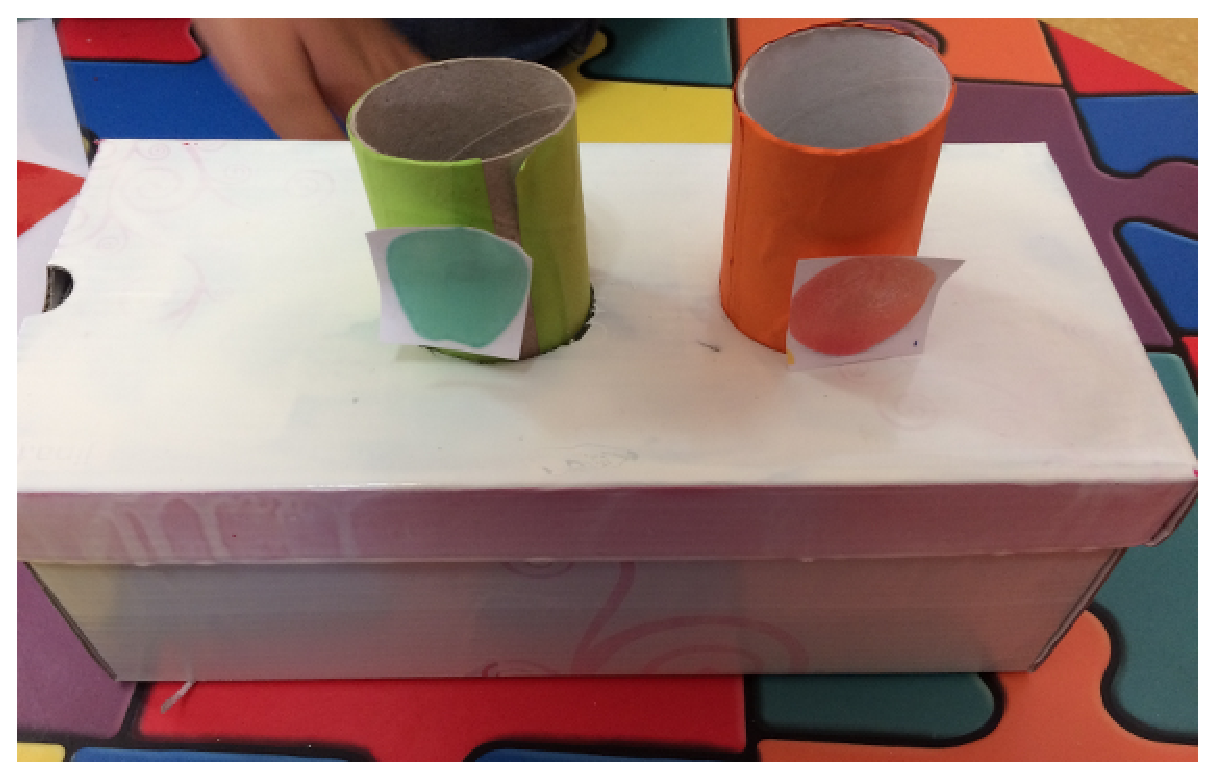
\includegraphics[height=3.3cm]{Nombres_et_calculs_did/Images/Num1_analyse_quatre_boite}
         &&
         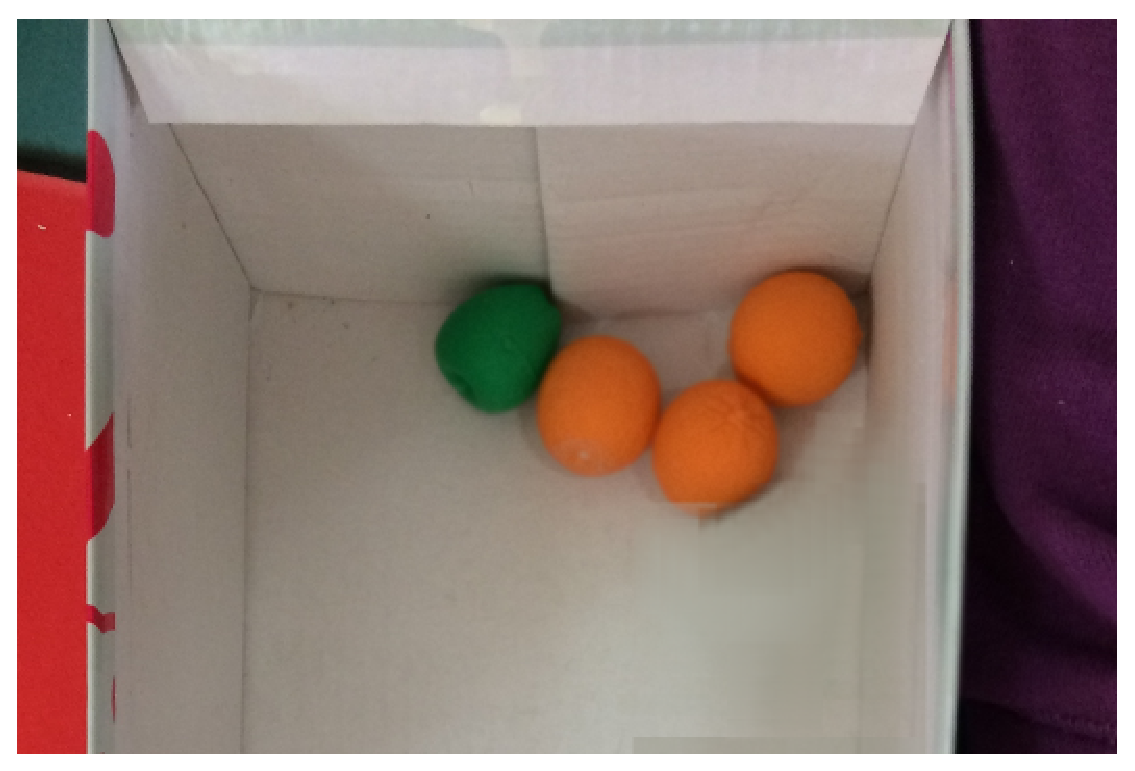
\includegraphics[height=3.3cm]{Nombres_et_calculs_did/Images/Num1_analyse_quatre_contenu}
         &&
         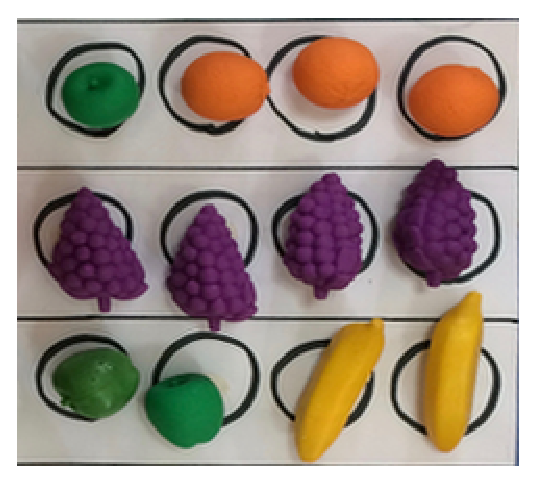
\includegraphics[height=3.3cm]{Nombres_et_calculs_did/Images/Num1_analyse_quatre_maison} \\
         L'élève possède une boite opaque avec 2 ouvertures par lesquelles il doit mettre 4 fruits à choisir parmi des pommes ou des oranges ; \newline
         &&
         il ouvre la boite, puis les dénombre : par exemple \og il y a une pomme et trois oranges, 1 et encore 3 ça fait 4 \fg ;
         &&
         il dispose ses fruits dans la \og maison du 4 \fg. \newline
         Puis, il répète l'opération avec d'autres fruits. \\ [3mm]
      \end{tabular}
      \item Les albums à calculer de {\it Rémi Brissaud, collection \og J’apprends les maths \fg, éditions Retz}. \\
      Ils s'utilisent progressivement et comporte trois types d'activité. \\ [3mm]
      \begin{tabular}{C{5}C{5}C{5}}
         \includegraphics[width=4.8cm]{Nombres_et_calculs_did/Images/Num1_analyse_quatre_souris}
         &
         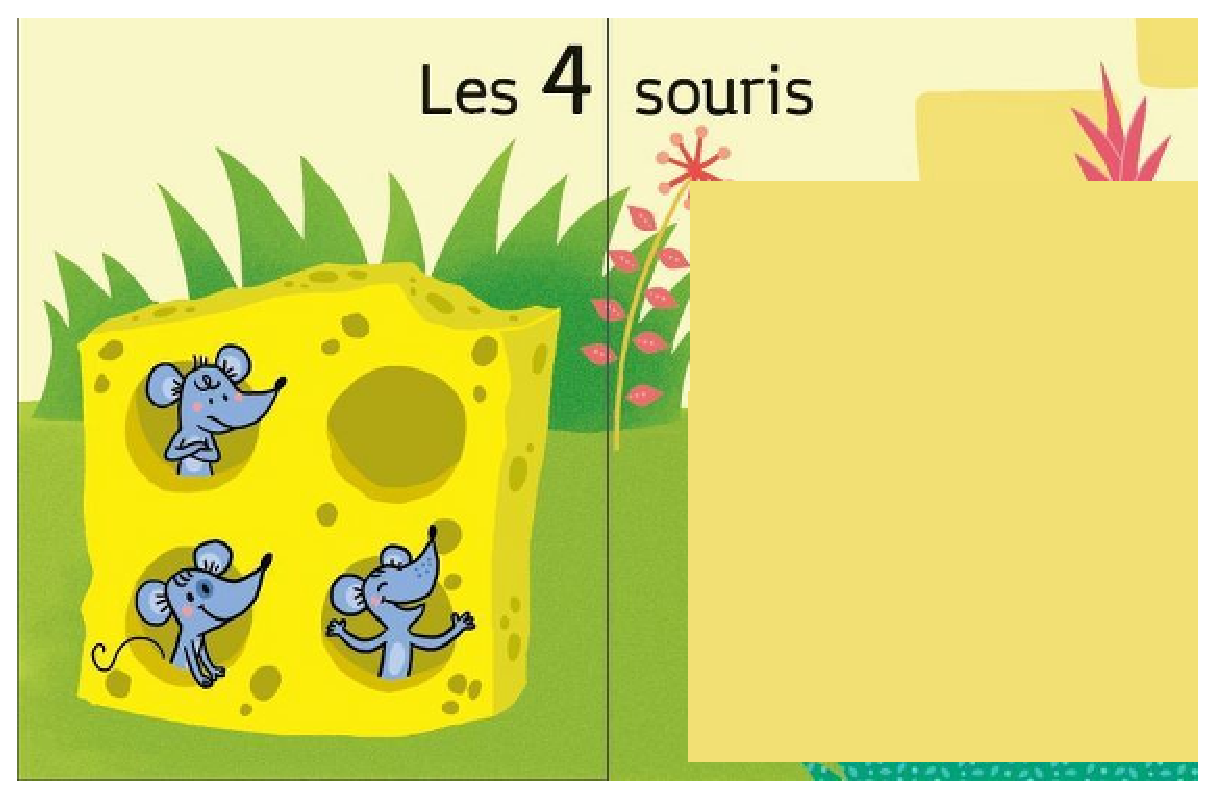
\includegraphics[width=4.8cm]{Nombres_et_calculs_did/Images/Num1_analyse_quatre_souris_g}
         &
         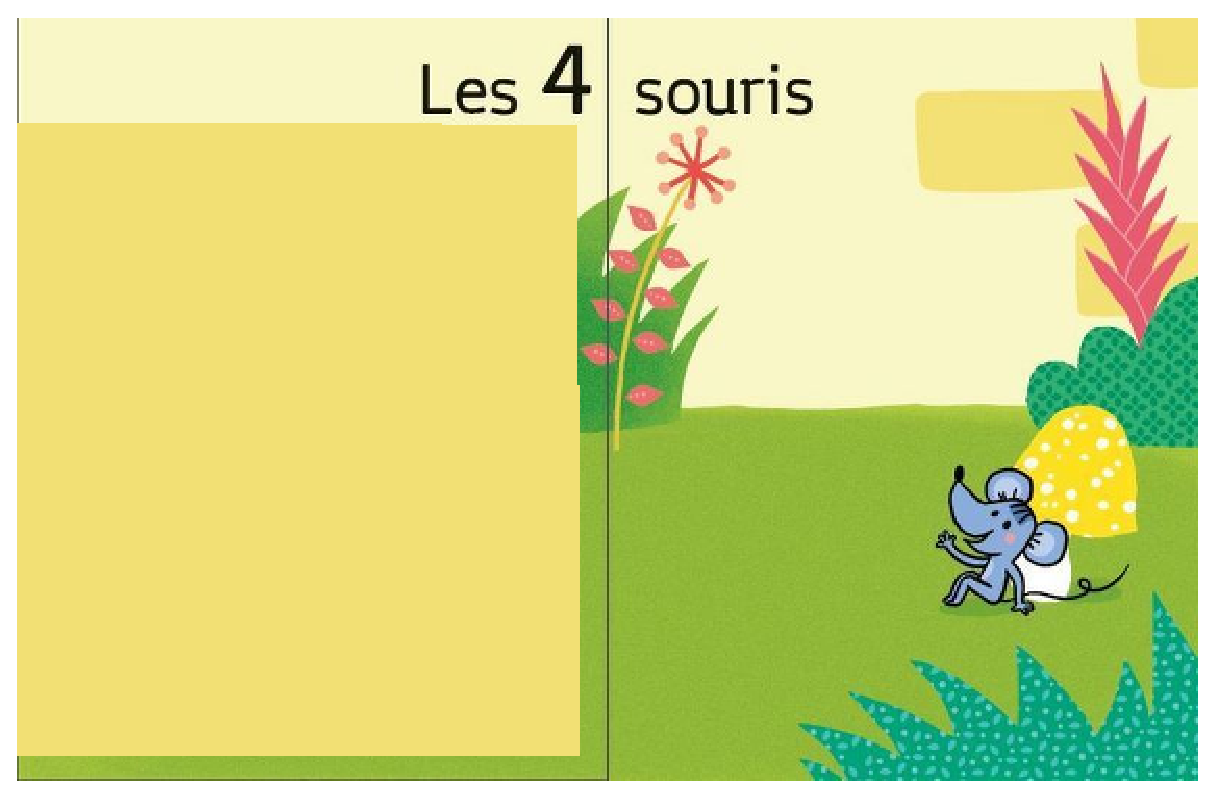
\includegraphics[width=4.8cm]{Nombres_et_calculs_did/Images/Num1_analyse_quatre_souris_d} \\
         Dans l'image, il y a 4 souris : 3 sont dans des trous de gruyère disposés comme les points du dé. Une est dans l'herbe sur l'autre page. 3 et encore 1, ça fait 4.
         &
         Il y a 4 souris mais on ne les voit pas toutes. \newline
         Combien y a-t-il de souris dans l'herbe sous le rabat ? 
         &
         Il y a 4 souris mais on ne les voit pas toutes. \newline
         Combien y a-t-il de souris dans le gruyère sous le rabat ? \\
      \end{tabular}      
   \end{itemize}
   \bigskip
   \item On peut citer plusieurs intérêts :
   \begin{itemize}
      \item travailler d'autres constellation moins classiques ;
      \item travailler le lien entre les différentes représentations des nombres : pour passer d'un nombre à son successeur, on ajoute 1 point à la droite de la configuration précédente sans en changer la disposition (sur un dé classique, le passage de 3 à 4 demande de modifier la disposition des points intégralement. Ici, il suffit de compléter le 3 par un point sur le coin vide);
      \item travailler les décompositions de manière visuelle : par exemple, 5 c'est 3 et encore 2 (si on lit verticalement) ou c'est 2 et encore 2 et encore 1 (si on lit horizontalement), ou encore c'est 4 et encore 1.
   \end{itemize}
\end{enumerate}
\end{corrige}


\Recreation
%%%%%%%%%%%%%%%%%%%%%%%%%%%%%%%%%

\setcounter{exercice}{0}
\begin{exercice*}[\fbox{C1} - Les Albums des premiers nombres pour ancrer le principe cardinal et la subitisation]
   Dans la collection \og J'apprends les maths \fg, Retz, par {\it Rémi Brissaud} :
   \begin{itemize}
      \item L'album 123 ;
      \item 1, 2 et 3 - PS ;
      \item \href{https://www.youtube.com/watch?v=AvEVhRyDZa8&feature=emb_logo}{L'album des premiers nombres 2, 3, 4 et 5}. 
   \medskip
   \end{itemize}
   Ce sont des albums avec rabats pour découvrir les premiers nombres en maternelle dans l’esprit des programmes de 2 020 en favorisant un authentique dénombrement, en évitant le comptage-numérotage, et en s'appropriant leurs décompositions. \\
   Le principe : parmi plusieurs collections, l'élève doit trouver celle qui a un nombre donné d'unités et justifier sa réponse en utilisant une décomposition du nombre.
   \begin{center}
      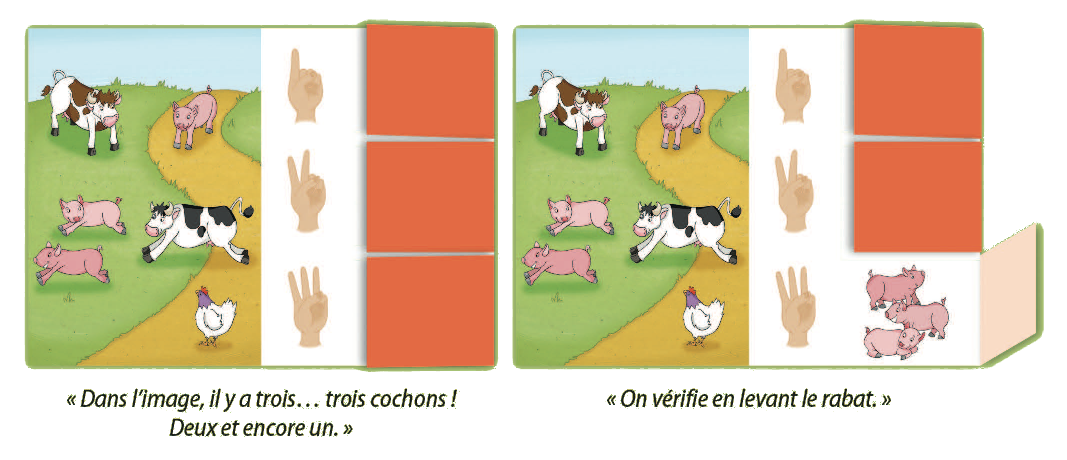
\includegraphics[width=13cm]{Nombres_et_calculs_did/Images/Num1_activites_123_cochons} \\
      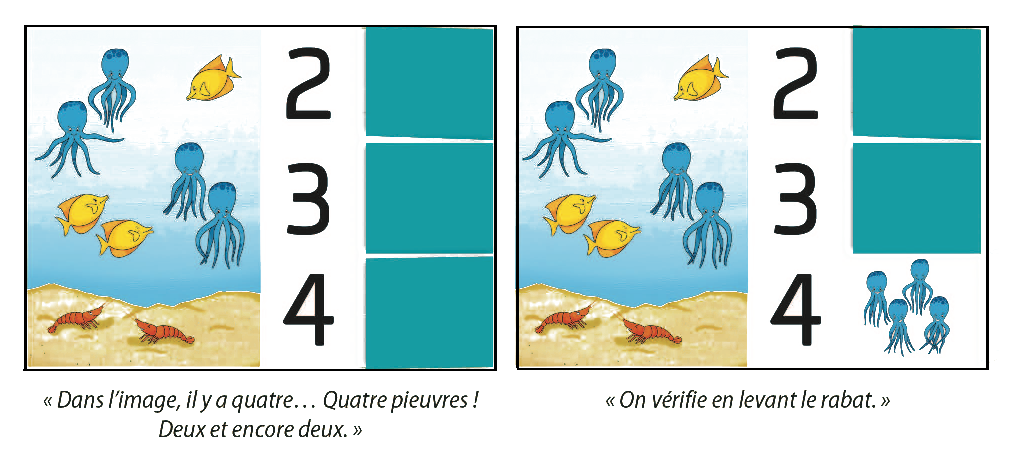
\includegraphics[width=13cm]{Nombres_et_calculs_did/Images/Num1_activites_123_pieuvres}
   \end{center}
\end{exercice*}

\medskip


\begin{exercice*}[\fbox{C1} - Les fiches à comparer pour comprendre le comptage et la correspondance terme à terme]
   Dans la collection \og J'apprends les maths \fg, Retz, par {\it Rémi Brissaud} :
   \begin{itemize}
      \item \href{http://extranet.editis.com/it-yonixweb/images/322/art/doc/4/4d22235f9031343337373530343434363934323630.pdf}{Je compte, tu compares, de 3 à 5 - PS-MS} ;
      \item \href{http://extranet.editis.com/it-yonixweb/images/322/art/doc/f/f2264616e731343337373530333832383731323539.pdf}{Je compte, tu compares, de 5 à 7 - MS-GS} ;
      \item \href{https://www.youtube.com/watch?v=8Iai1uyfaFg&feature=emb_logo}{Je compte... tu compares MS-GS}.
   \end{itemize}
   \medskip
   Un matériel collectif, destiné aux classes de PS à GS, pour comprendre le comptage. Il offre un type de situation pédagogique où, à partir de la seule écoute du comptage oral de deux collections, les enfants sont amenés à découvrir une règle simple pour déterminer si ces collections ont autant d’éléments : lorsque les deux comptages s’arrêtent au même mot, les collections ont le même nombre d’éléments et si l’un des comptages \og va plus loin \fg{} que l’autre, c’est celui de la collection la plus nombreuse. \\
   Intérêts : comprendre dans le même temps comment l’usage d’une liste ordonnée de mots-nombres permet de mesurer la taille d’une collection, accéder aux décompositions d'un nombre grâce à la comparaison.
   \begin{center}
      \fbox{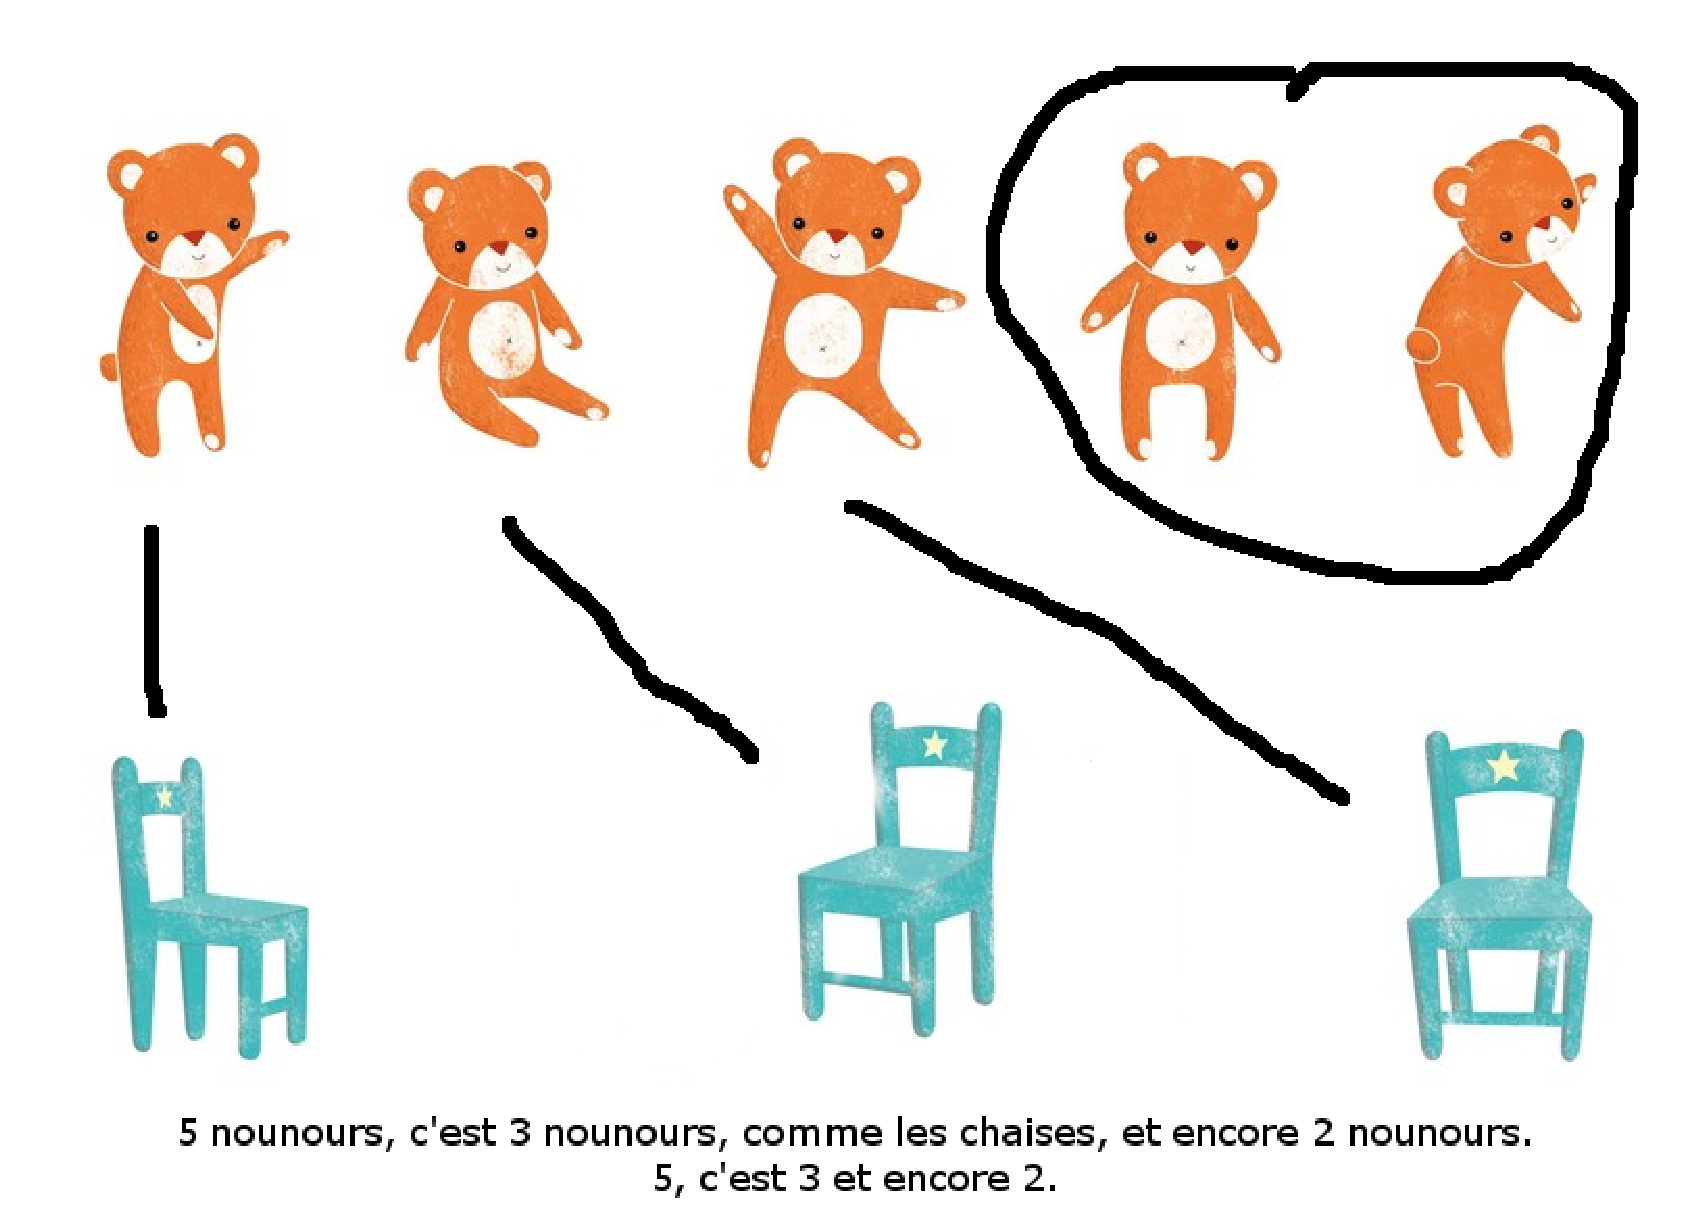
\includegraphics[width=8cm]{Nombres_et_calculs_did/Images/Num1_activites_JCTC_ours_chaise_final}}
      \qquad
      \fbox{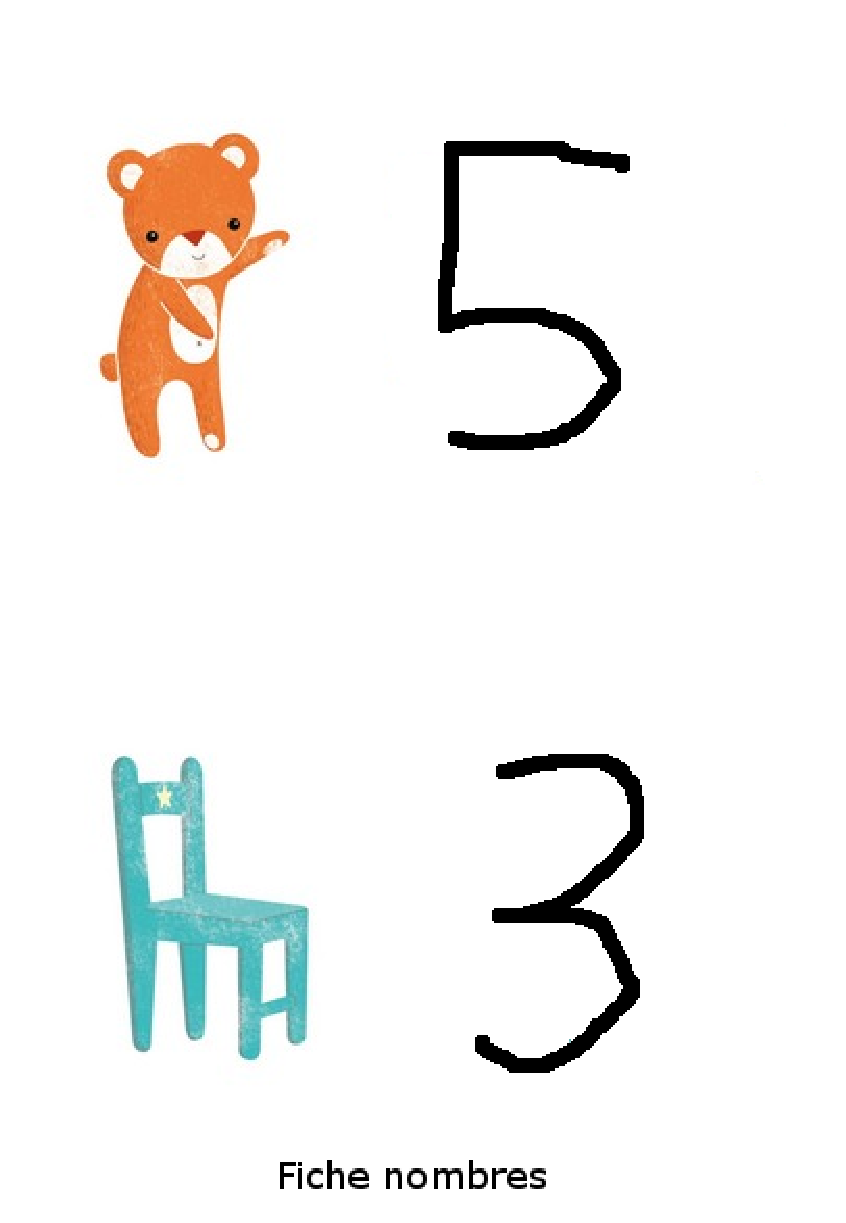
\includegraphics[width=5cm]{Nombres_et_calculs_did/Images/Num1_activites_JCTC_fiche_nombre}}
   \end{center}
\end{exercice*}

\bigskip


\begin{exercice*}[\fbox{C1} - Les albums à calculer pour comprendre et apprendre les décompositions]
   Dans la collection \og J'apprends les maths \fg, Retz, par {\it Rémi Brissaud} :
   \begin{itemize}
      \item L'album à calculer GS (premier et deuxième) ;
      \item Albums à calculer 3,4,5,6,7 avec les animaux du cirque ou du jardin - MS-GS ;
      \item Albums à calculer 5,6,7,8,9,10 avec les animaux de la maison - GS ;
      \item Fiches à calculer 3,4,5,6,7 avec les animaux du cirque ou du jardin MS-GS ;
      \item \href{https://www.youtube.com/watch?v=F_g4T3C0ad0&feature=emb_logo}{Fiches à calculer 5,6,7,8,9,10 avec les animaux de la maison - GS}.
   \end{itemize}
   \medskip
   Les albums et fiches à calculer permettent de travailler toutes les décompositions des nombres de 3 à 10, en classe entière, en petits groupe (les enfants jouent à plusieurs, avec un meneur de jeu), ou en remédiation individuelle. \\
   Le principe : les élèves doivent retrouver pour chaque page le nombre d'animaux manquant connaissant le nombre total d'animaux en utilisant les rabats de la couverture. Les animaux de la page de gauche sont disposés en constellations.
   \begin{center}
      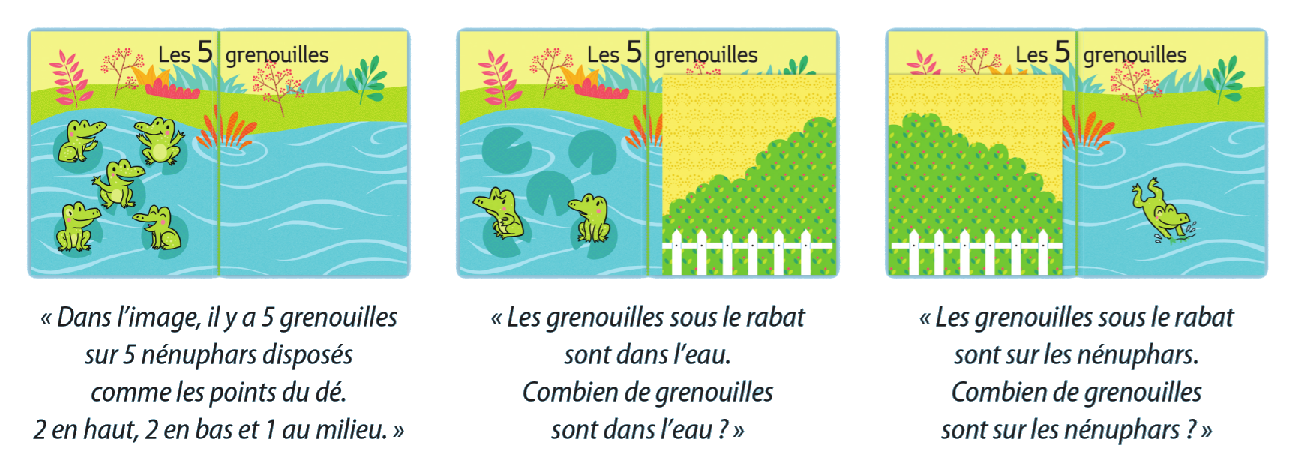
\includegraphics[width=17cm]{Nombres_et_calculs_did/Images/Num1_activites_album_calculer_grenouilles}
   \end{center}
\end{exercice*}

\bigskip


\begin{exercice*}[\fbox{C1} - Fabriquer des boites à nombres]
   \og L'atelier boites à compter \fg{} est un jeu éducatif proposé par {\it Nathan} et permet aux enfants d'apprendre à dénombrer, à réaliser des collections de quantité donnée, de reconnaître différentes représentations des nombres. \\
   \begin{center}
      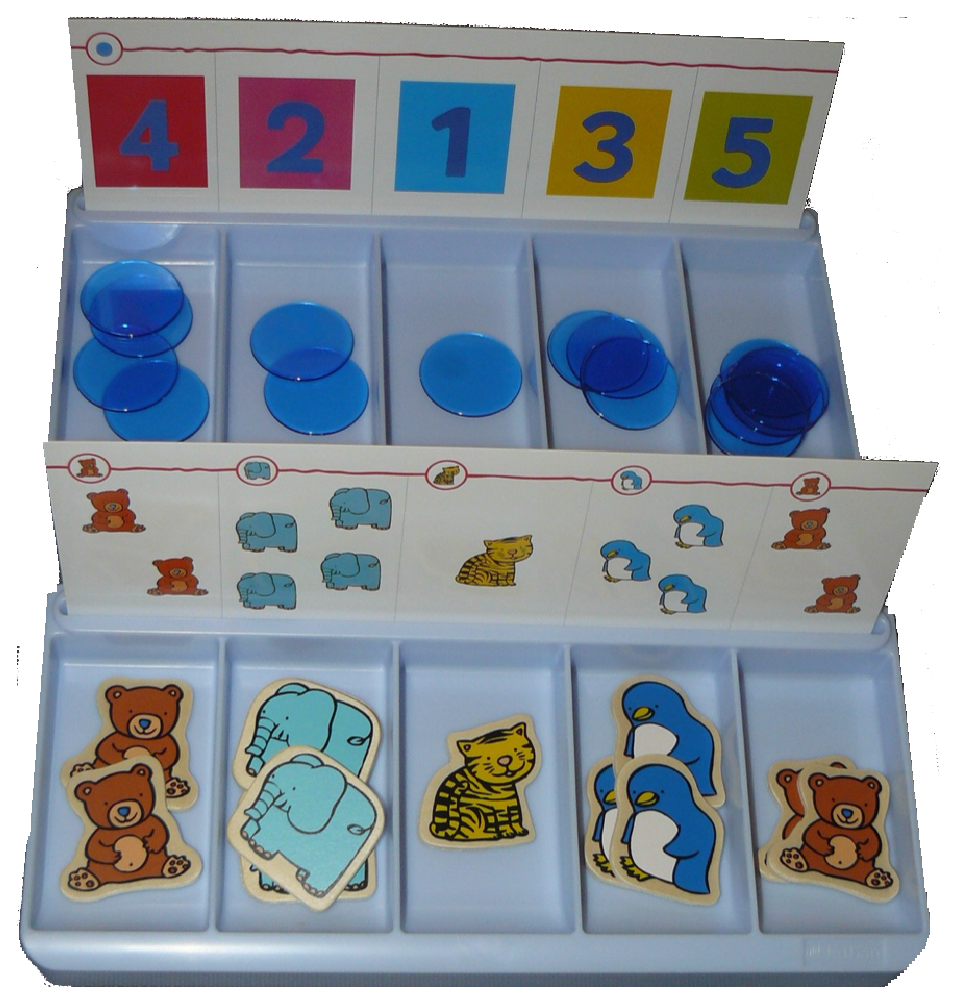
\includegraphics[height=6.5cm]{Nombres_et_calculs_did/Images/Num1_activites_boite_compter_Nathan} \qquad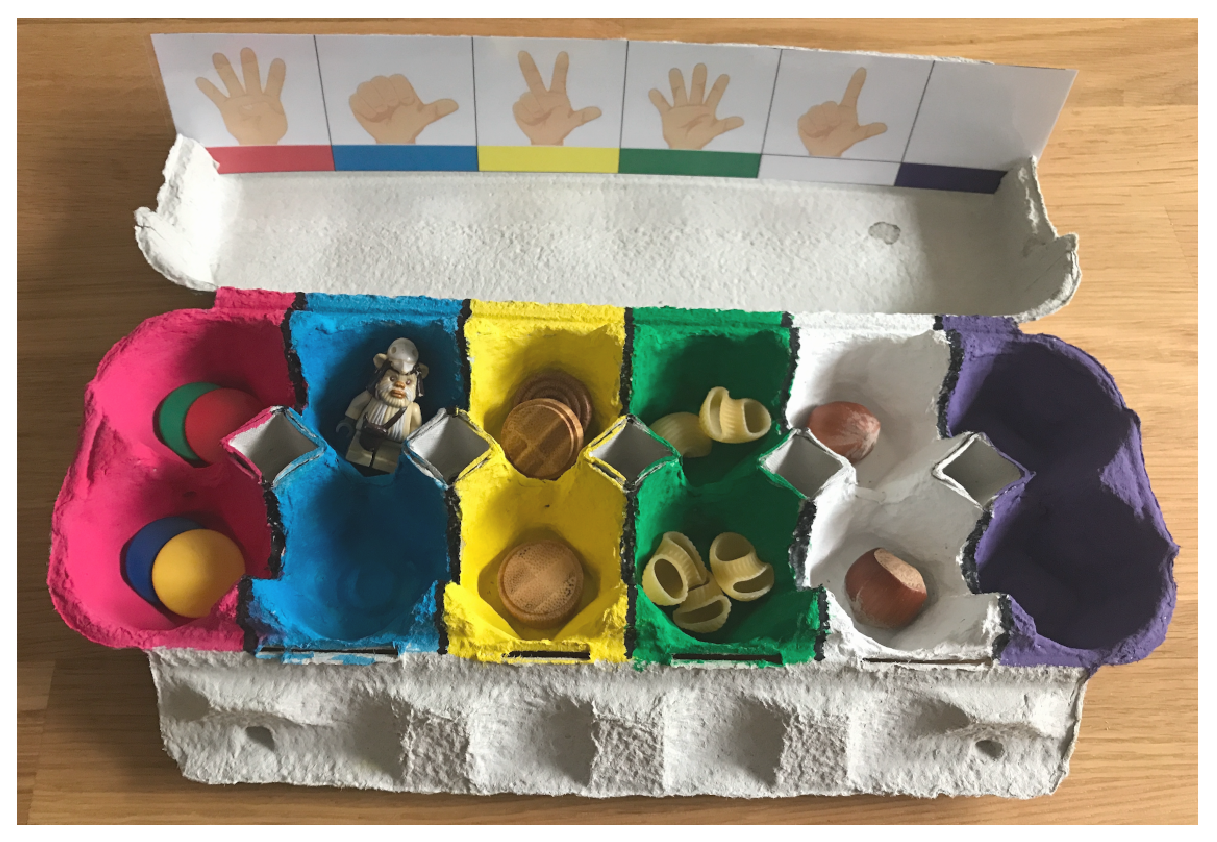
\includegraphics[height=6.5cm]{Nombres_et_calculs_did/Images/Num1_activites_boite_oeufs_nombres}
   \end{center} \bigskip
 
   Les élèves ont devant eux une boite à nombres, ainsi qu'une fiche et ils doivent reproduire la quantité donnée dans la case correspondante. Avec un budget rikiki, il est tout à fait possible de créer des boites à nombres à l'aide, par exemple, de boites à \oe ufs et de créer ses propres fiches en fonction de son niveau de classe.

   Les variables didactiques sur lesquelles on peut jouer sont les suivantes : 
   \begin{itemize}
      \item Les nombres abordés : 1 à 3 ; 1 à 5 ; 5 à 7 ; 5 à 10 ; 1 à 10\dots
      \item La représentation : digitale, constellation, dé, chiffrée, quadrillée\dots
      \item Les objets représentés : animaux, points, objets de la classe\dots
      \item La taille des objets.
      \item La variété des objets sur une même carte.
      \item Le thème de la fiche : plusieurs représentations du même nombre, représentations de nombres différents à l'aide de mêmes représentants, représentations variées\dots
      \item Les objets à utiliser : jetons, animaux, légos, couleurs différentes\dots
      \item L'éloignement des objets : sur la table, au fond de la classe, à prendre en une seule fois\dots \\
   \end{itemize}
   \begin{center}
     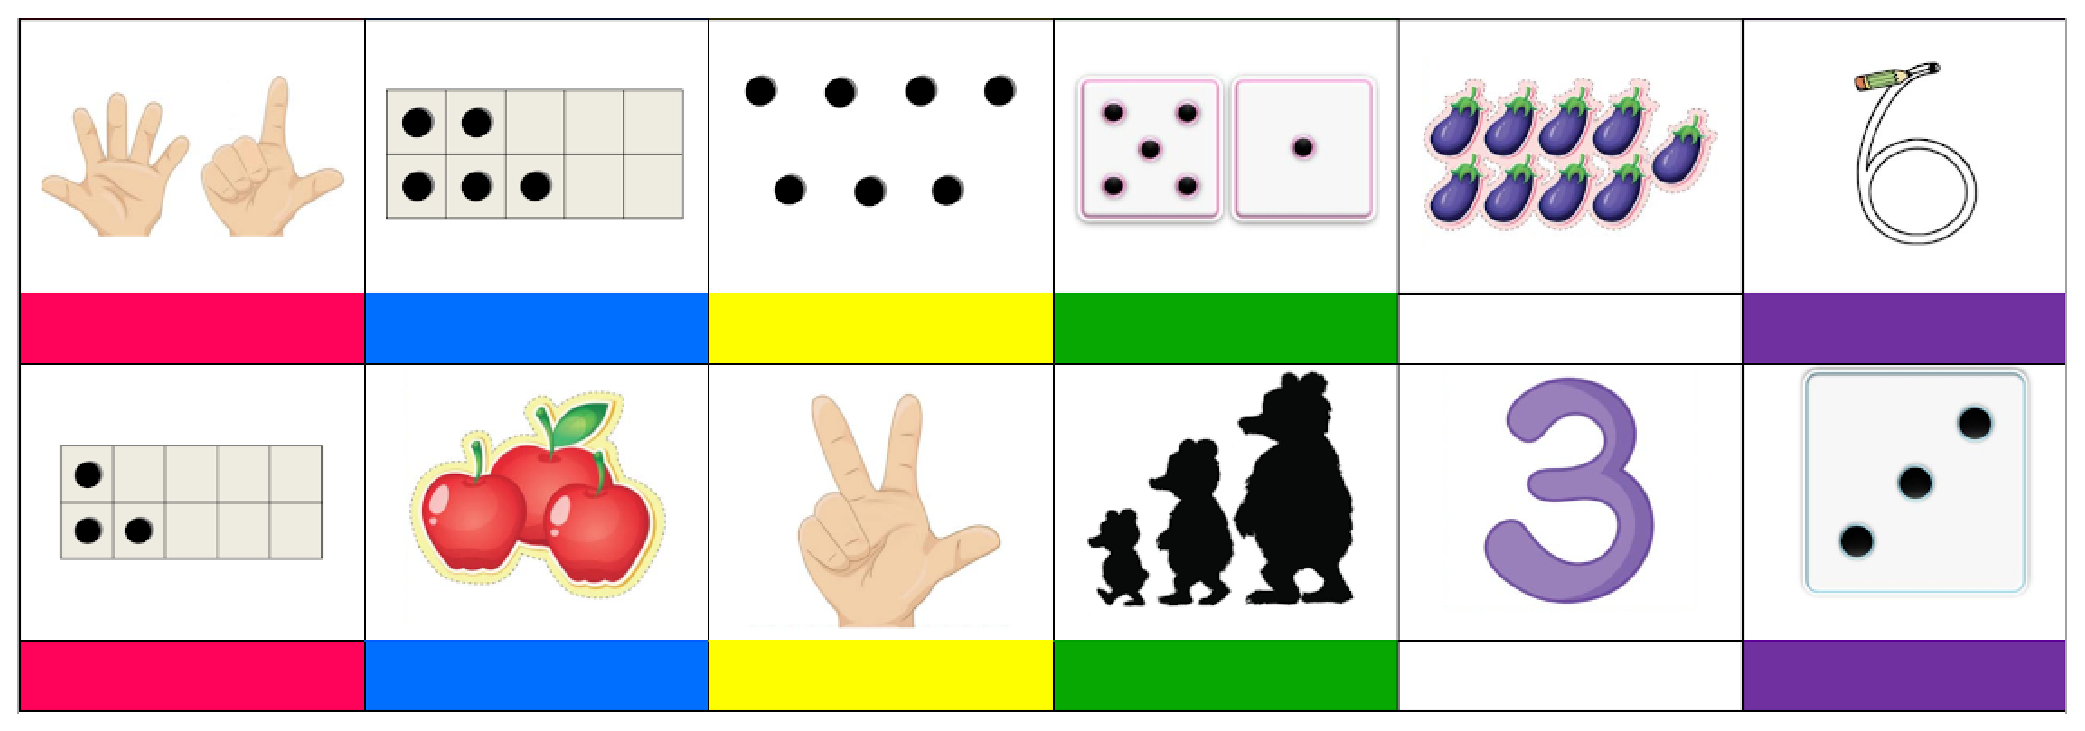
\includegraphics[width=16cm]{Nombres_et_calculs_did/Images/Num1_activites_fiches_boite_oeufs}
   \end{center}
\end{exercice*}

\bigskip


\begin{exercice*}[\fbox{C1} - La piste au trésor]
   Dans le manuel \og Découvrir les maths \fg{} en MS, de {\it Dominique Valentin}, on trouve la situation {\it Piste au trésor}. \\ 
   {\bf Objectif :} Apprendre à choisir une quantité en fonction d'un but à atteindre. \\
   {\bf Compétences travaillées :} Évaluer et comparer des collections d’objets avec des procédures numériques ou non numériques. Quantifier des collections jusqu’à dix au moins ; les composer et les décomposer par manipulations effectives puis mentales. Dire combien il faut ajouter ou enlever pour obtenir des quantités ne dépassant pas dix. Parler des nombres à l’aide de leur décomposition. \\
   {\bf But à atteindre :} être le premier à remplir exactement sa grille en plaçant un jeton dans chaque case, sans en avoir pris trop. \\
   {\bf Matériel :} Une piste de jeu, deux dés avec les couleurs du plateau de jeu, une boîte avec des jetons, des tickets \og trésor \fg, une grille réponse de 10 cases par enfant. {\it\blue \href{https://dessinemoiunehistoire.net/wp-content/uploads/2017/02/La-piste-au-trésor-jeu-de-numération-maternelle.pdf}{Matériel à imprimer}}.
   \begin{center}
      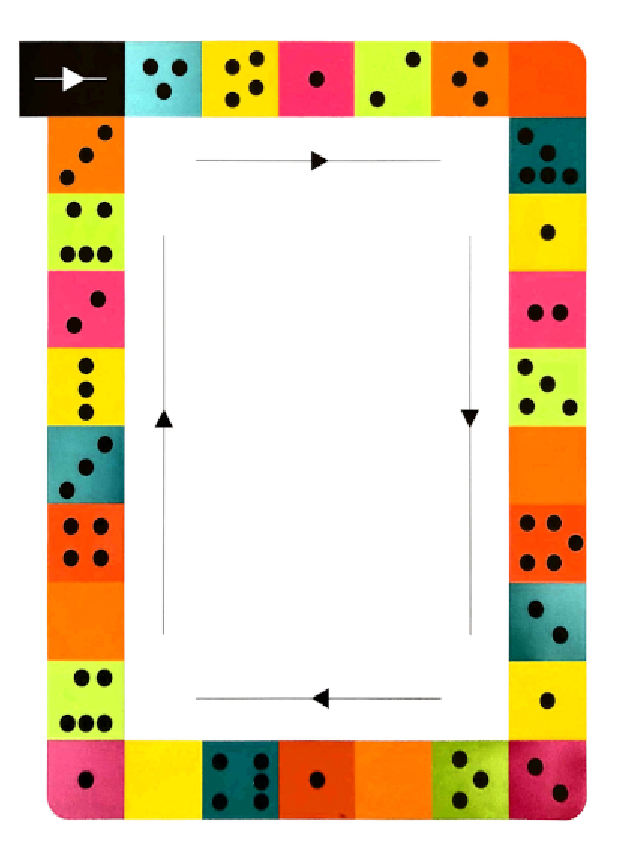
\includegraphics[width=5cm]{Nombres_et_calculs_did/Images/Num1_activites_piste_1} \quad 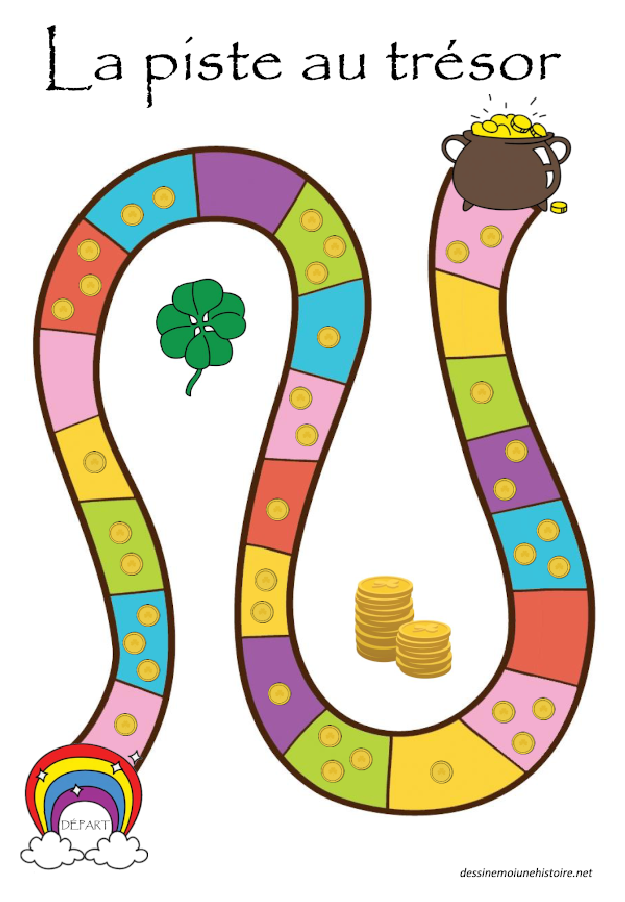
\includegraphics[width=5cm]{Nombres_et_calculs_did/Images/Num1_activites_piste_2}
   \end{center}
   {\bf Activité 1 : Avec un seul dé, appropriation des règles et du but du jeu}. \\
    Le premier joueur lance le dé et avance son pion sur la case de la couleur indiquée par le dé. Il prend alors autant de jetons dans sa boîte qu’il y en a de dessinés sur la case où est arrivé son pion. Il les pose sur son plateau. Il doit alors décider s’il reste sur sa grille assez de cases vides pour y poser les jetons qu’il vient de gagner. Si c’est le cas, il les place sur sa grille. Dans le cas contraire, s’il est capable de s’apercevoir qu’il aura trop de jetons avant de commencer à les poser, il peut les refuser et les remettre dans sa boîte. Si le joueur a pris plus de jetons que ne peut en contenir sa grille, la grille est entièrement vidée. Le joueur doit recommencer à la remplir, sans revenir au début de la piste. Les joueurs jouent alternativement jusqu’à ce que l’un d’eux aie rempli sa grille (et non jusqu’à ce que l’un deux soit arrivé au bout de la piste). Il est possible de faire plusieurs tours de piste. Chaque joueur a un observateur chargé du bon respect des règles (et non du meilleur choix). \\
   {\bf Activité 2 : Avec deux dés, choisir pour gagner}. \\
   Avec deux dés, le jeu porte sur la stratégie d’anticipation. Chaque joueur lance à son tour les deux dés et choisit la couleur qui lui permet de ramasser la quantité de jetons qui lui convient en avançant sur la case de la couleur choisie la plus proche. Si les deux dés tombent sur la même couleur, le joueur relance un des deux dés. Il arrive qu’aucun des deux dés ne convienne (quantités trop importantes pour le nombre de cases à remplir) ; le joueur peut passer son tour en disant pourquoi. Comme dans le cas du jeu avec un seul dé, le joueur qui a pris trop de jetons perd, et sa grille est vidée. Lorsqu’un joueur a rempli sa grille, il gagne un ticket \og trésor \fg. En fin de jeu, le nombre de tickets gagnés par chaque joueur est comparé. Celui qui possède le plus de tickets remporte la partie.
\end{exercice*}

\bigskip


\begin{exercice*}[\fbox{C2} - Les fourmillions pour comprendre le codage des nombres et notre système de numération]

D'après \og Apprentissages numériques et résolution de problèmes \fg, Hatier ERMEL, de {\it Roland Charnay} (page 333 pour le CP, 316 pour le CE1). Le terme [fourmillions] est emprunté au livre de {\it Fynn}, \og Anna et Mister God \fg, Le Seuil, et défini comme un mot élastique que l'on peut étirer à l'infini pour désigner un très grand nombre. C'est la traduction française du mot anglais inventé par l'auteur : [squillions]. \\

\begin{center}
   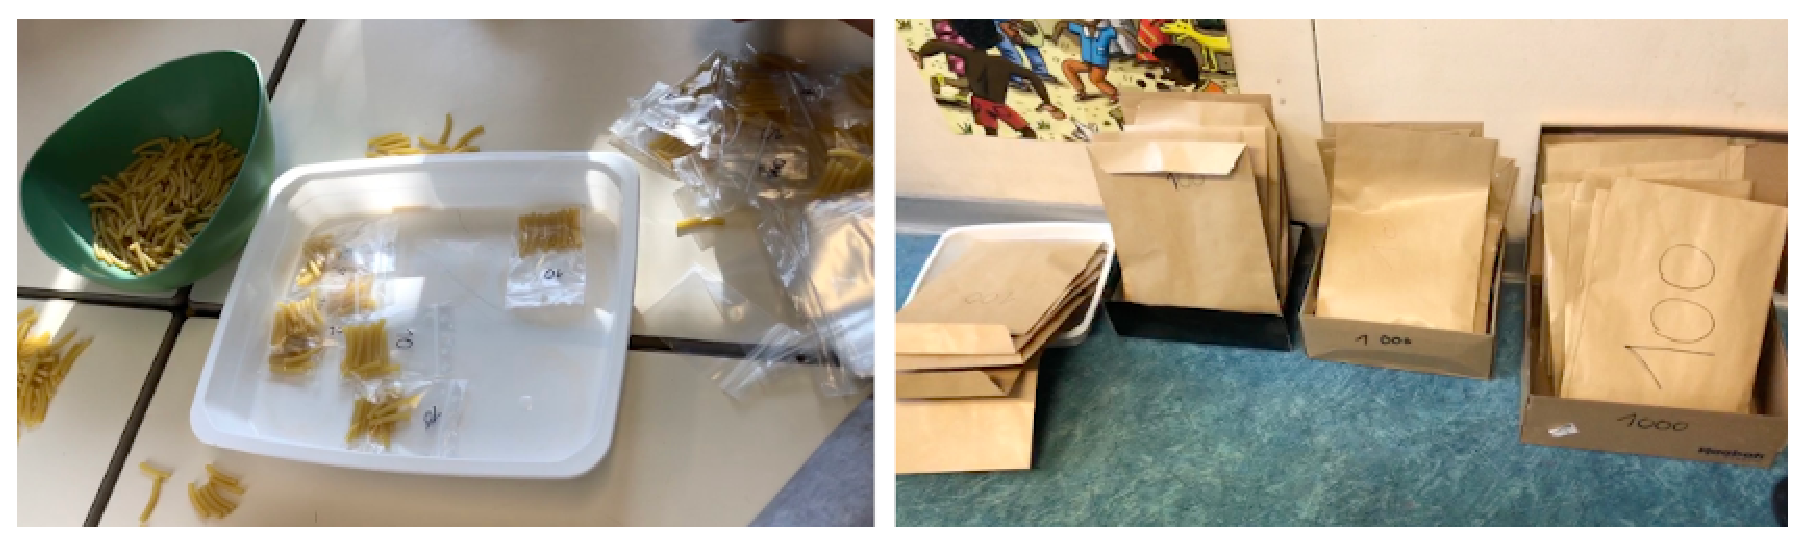
\includegraphics[width=15cm]{Nombres_et_calculs_did/Images/Num1_activites_fourmillions}
\end{center}

{\bf Objectifs}
\begin{itemize}
   \item Faire percevoir la nécessité de développer une stratégie plus efficace que le dénombrement un à un.
   \item Amener les enfants à organiser une collection en utilisant les groupements par dix, afin d'obtenir un dénombrement plus fiable.
   \item Faire admettre que ce mode de groupement peut se réitérer (récursivité des groupements).
   \item Donner du sens aux mots \og unité \fg, \og dizaine \fg, \og centaine \fg, éventuellement \og mille \fg.
   \item Écrire 100 sous la forme : $10 + 10 + 10 + 10 + 10 + 10 + 10 + 10 + 10 + 10$.
   \item Permettre la production d'une écriture de nombre de trois à quatre chiffres (nombre écrit et lu avec l'enseignant).
\end{itemize}
{\bf Domaine numérique travaillé} : les nombres à deux, trois chiffres (et parfois au-delà). \\
{\bf Période idéale} : P4 pour le CP, P2 pour le CE1 et P1 pour le CE2. \\
{\bf Mise en place de la situation} : une ou plusieurs séances au cours desquelles on pose le problème du dénombrement d'une collection importante d'objets récupérés depuis le début de l'année par les enfants à la demande du maître par exemple. Cette collection doit contenir plus de 1\,300 éléments. \\
{\bf Matériel} :
\begin{itemize}
   \item des objets en quantité : bouchons, haricots, bûchettes, des trombones, pâtes\dots ;
   \item des élastiques, des sacs en plastique, des enveloppes, des boîtes\dots{} permettant de contenir les objets.
\end{itemize}

\begin{enumerate}
   \item {\bf Première phase : émergence de questions (phase collective).} \\
   On pose le problème aux enfants réunis autour du tas d'objets: \og Combien y a-t -il d'allumettes, ou pois\dots)? \fg \\
   L'enseignant recueille les réponses, les débuts de procédures, les réactions, les remarques de tous ordres, comme : \og On les compte un par un \fg ; \og On ne peut pas savoir, c'est trop long à compter \fg ; \og On en prend 5 chacun, on sait compter de 5 en 5 \fg ; \og On compte 2 par 2 \fg ; \og C'est pas assez par 5. On va les mettre par 10 et on aura 10, 20, 30, 40\dots \fg Si l'idée de grouper par dix ne sort pas, l'enseignant devra la proposer. \medskip

   \item {\bf Deuxième phase : mise en place de la procédure de groupement (travail de groupes).}
   \begin{enumerate}
      \item {\bf Étape 1 : les dizaines.} La moitié des enfants fabrique des paquets de 10 objets (les remplisseurs). Les autres contrôlent ces paquets. Lorsque ce travail est fini, on range les paquets et on met en réserve les objets isolés.
      \item {\bf Étape 2 : les centaines.} Quand tous les paquets de dix sont prêts, on fait des sacs de 10 paquets de dix. On range les sacs de 100, on range les paquets de dix non regroupés et les objets isolés.
      \item{\bf Étape 3 : les milliers.} On regroupe tous les enfants autour des sacs et on fait des boîtes de mille objets. Cette phase de mise en place de la procédure de groupements et de sa réitération permet aux enfants de bien saisir l'organisation des groupements. Elle s'accompagne de langage, de remarques que l'enseignant souligne, qu'il reformule, qu'il renvoie au groupe classe, comme : \og 10, 20, 30, 40, 50, 60, 70, 80, 90, 100 objets pour ce sac \fg ; \og 10 sacs de 10, c'est 100, c'est une centaine\fg{} ; \og il y a 10 objets dans les petites enveloppes, 10 petites enveloppes dans les grandes, 10 grandes enveloppes dans les sacs, on pourrait mettre 10 sacs dans des plus grands \fg. \medskip
   \end{enumerate}

   \item {\bf Troisième phase : productions d'écritures.} \\
   Lorsque la collection est ainsi organisée, ou après chaque étape, l'enseignant propose de chercher un message à noter sur le sac de cent, puis sur la boîte de mille pour se rappeler de leur contenu. Quand les élèves l'ont fait, il affiche les écrits les plus caractéristiques que les enfants déchiffrent et critiquent. \\
   Après avoir reposé la question : \og Combien y a-t-il d'objets?\fg{}, l'enseignant demande d'écrire le nombre d'objets de la collection. On ne vise pas, à ce moment-là, la maîtrise de cette écriture, mais bien plutôt la découverte de son existence. L'enseignant acceptera aussi bien : \og 1 sac de 1\,000 objets, 3 sacs de 100 objets, 8 sacs de 10 objets, 7 objets \fg ; \og $1\,000 + 100 + 100 + 100 + 10 + 10 + 1 0 + 1 0 + 1 0 + 1 0 + 10 + 1 0 + 7$ \fg ; \og $1\,000 + 300 + 80 + 7$ \fg \\
   Si l'écriture 1\,387 n'est pas proposée par un enfant, elle l'est par l'enseignant qui la présente comme l'écriture \og la plus courte\fg{}, ou l'écriture \og habituelle\fg{} de ce nombre. \medskip

   \item {\bf Quatrième phase : le compteur vivant.} \\
   La collection continue à évoluer. L'enseignant demande aux enfants de récolter de nouveau des objets ayant servi à l'activité initiale. Chaque matin, l'enseignant relève les objets apportés et propose aux enfants de chercher quel est le nombre des éléments de la collection après cet ajout. \\
   Quatre enfants font fonctionner un \og compteur vivant\fg{} face au reste de la classe. Ils \og sont\fg{} les roues du compteur : roue des unités, dizaines, centaines et mille. Ils disposent de cartons de bristol ordonnés sur lesquels sont écrits les chiffres de 0 à 9. Ils changent la valeur des chiffres de leur roue à bon escient. \\
   Les mots \og dizaine\fg{}, \og centaine\fg{} sont utilisés chaque fois que nécessaire; l'écriture du nombre à l'aide des \og roues\fg{} du compteur et mise en évidence.  
   \end{enumerate}
\end{exercice*}

\bigskip


\begin{exercice*}[\fbox{C2} - Des jeux pour travailler la numération] 
\bigskip
\begin{tabular}{p{8cm}|p{8cm}}
   {\bf La bataille des dizaines et des unités} \newline
   \href{http://www.les-coccinelles.fr/lienpage2/numeration/outils/batailledizaineunitejusqua50.pdf}{\it\blue Lien vers le site \og Les coccinelles \fg.} \newline
   \begin{center}
      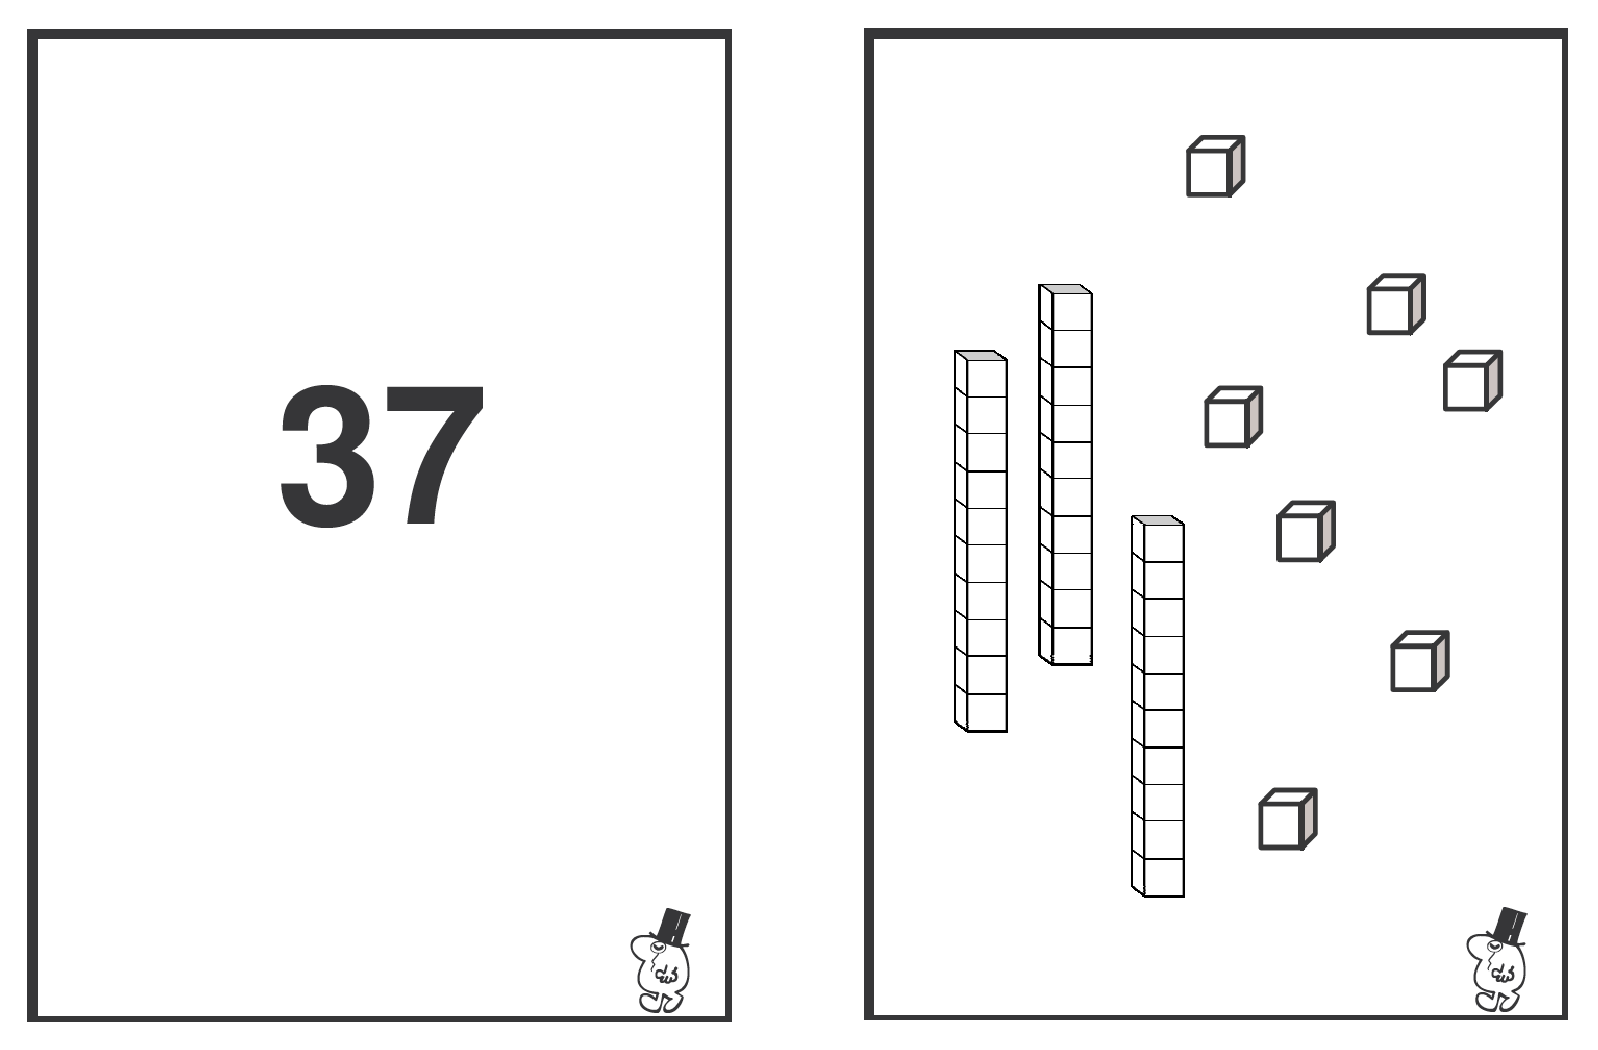
\includegraphics[height=3.5cm]{Nombres_et_calculs_did/Images/Num1_activites_dizaines_unites}
   \end{center}
   &
   {\bf Le jeu des neuf familles de la numération} \newline
   \href{https://lutinbazar.fr/jeu-des-9-familles-nombres-inferieurs-a-100/}{\it\blue Lien vers le site \og Lutin bazar \fg.} \newline
   \begin{center}
      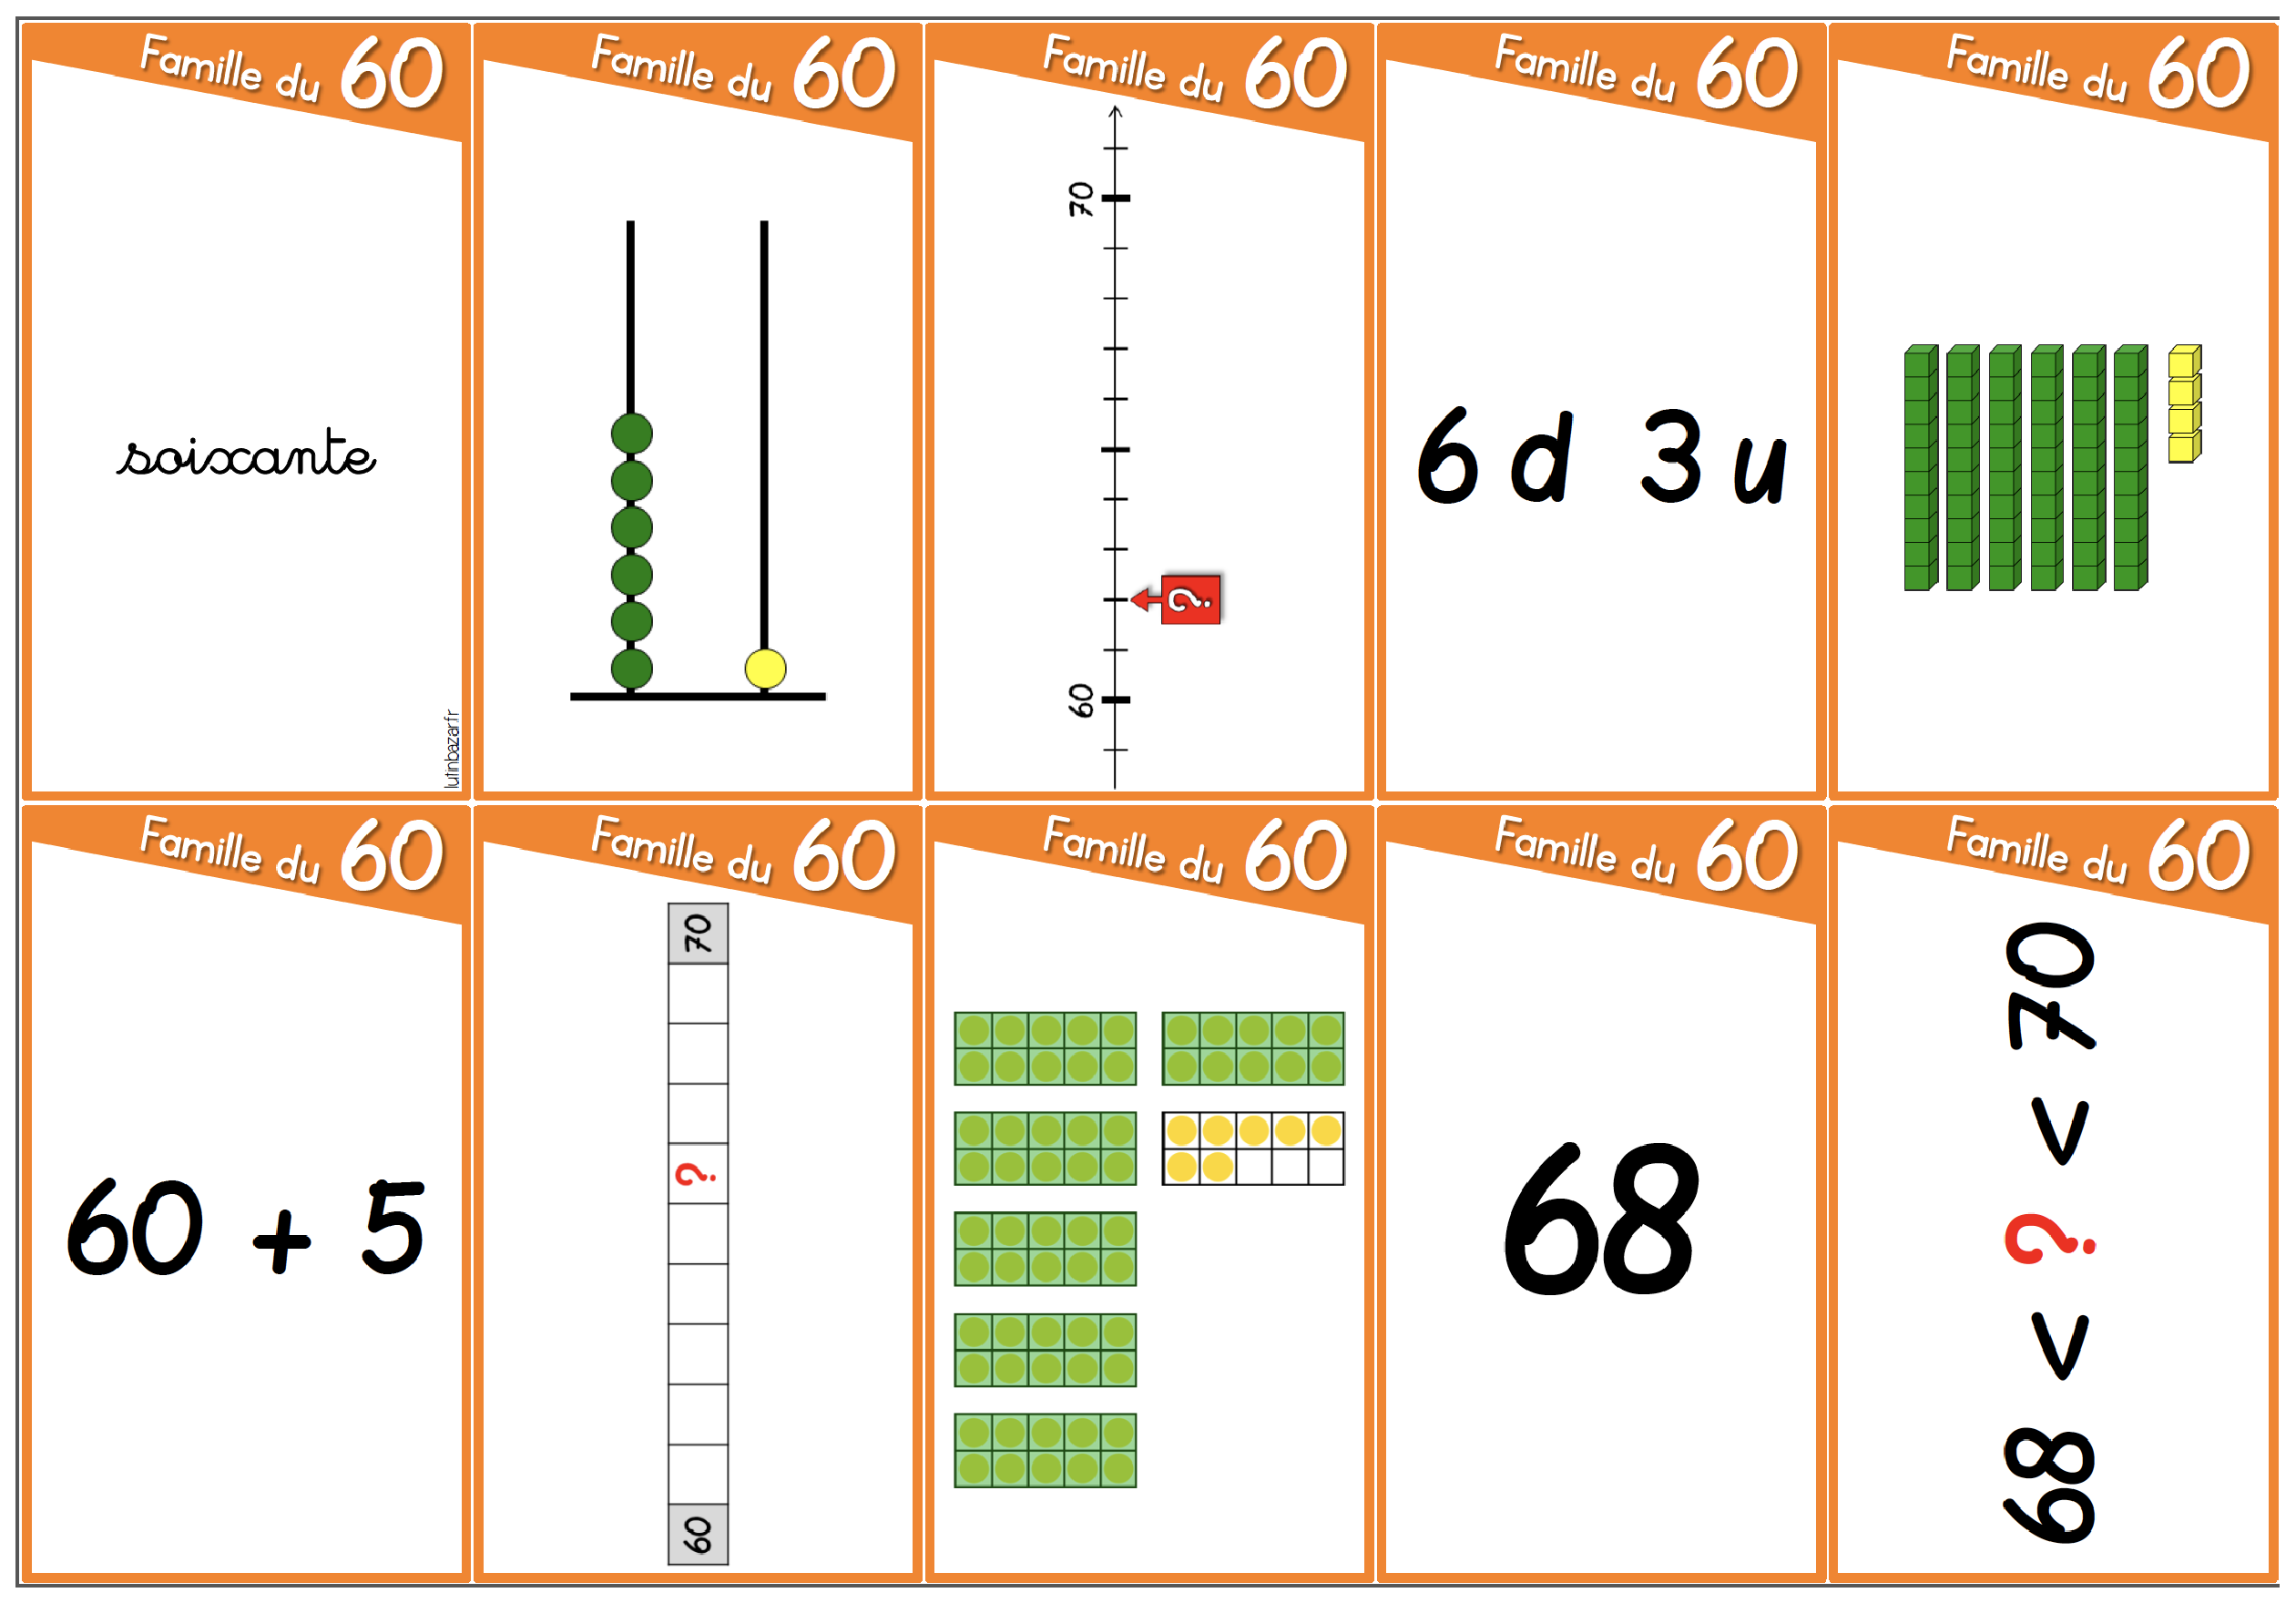
\includegraphics[height=3.5cm]{Nombres_et_calculs_did/Images/Num1_activites_neuf_familles}
   \end{center}
   \\
   {\bf Compétences travaillées} : comparer deux nombres, savoir décomposer et recomposer un nombre inférieur à 50 en dizaines et unités.
   &
   {\bf Compétences travaillées} : utiliser diverses représentations des nombres jusqu'à 100, passer d’une représentation à une autre.
   \\
   {\bf Principe du jeu} : jeu de bataille.
   &
   {\bf Principe du jeu} : jeu des sept familles.
   \\
\end{tabular}
\end{exercice*}

\bigskip


\begin{exercice*}[\fbox{C2/C3} - Utilisation de bouliers et d'abaques pour consolider la numération]
Les abaques (du latin {\it abacus}, emprunté au grec {\it abax}, \og table à calcul \fg) sont utilisés depuis des millénaires dans différents pays du monde et permettent une représentation aisée des nombres en fonction de leur position. Il en existe de différents type, par exemples, le boulier chinois et l'abaque à jetons.
\begin{enumerate}
   \item {\bf Le boulier chinois} \\
   Le boulier chinois est aussi appelé {\it su\`an p\'an} signifiant littéralement \og planchette à calcul \fg. \\
   Il possède habituellement 13 tiges et s’utilise posé à plat. On affecte à l'une des tiges la valeur de l'unité. Une boule est activée lorsqu'on l’approche de la barre transversale. Elle prend alors une valeur dépendant de la tige et de la partie (supérieure ou inférieure) sur laquelle elle est placée. L'écriture d'un nombre n'est pas unique, mais elle est optimisée lorsqu'aucune tige n'est vide.
   \begin{center}
      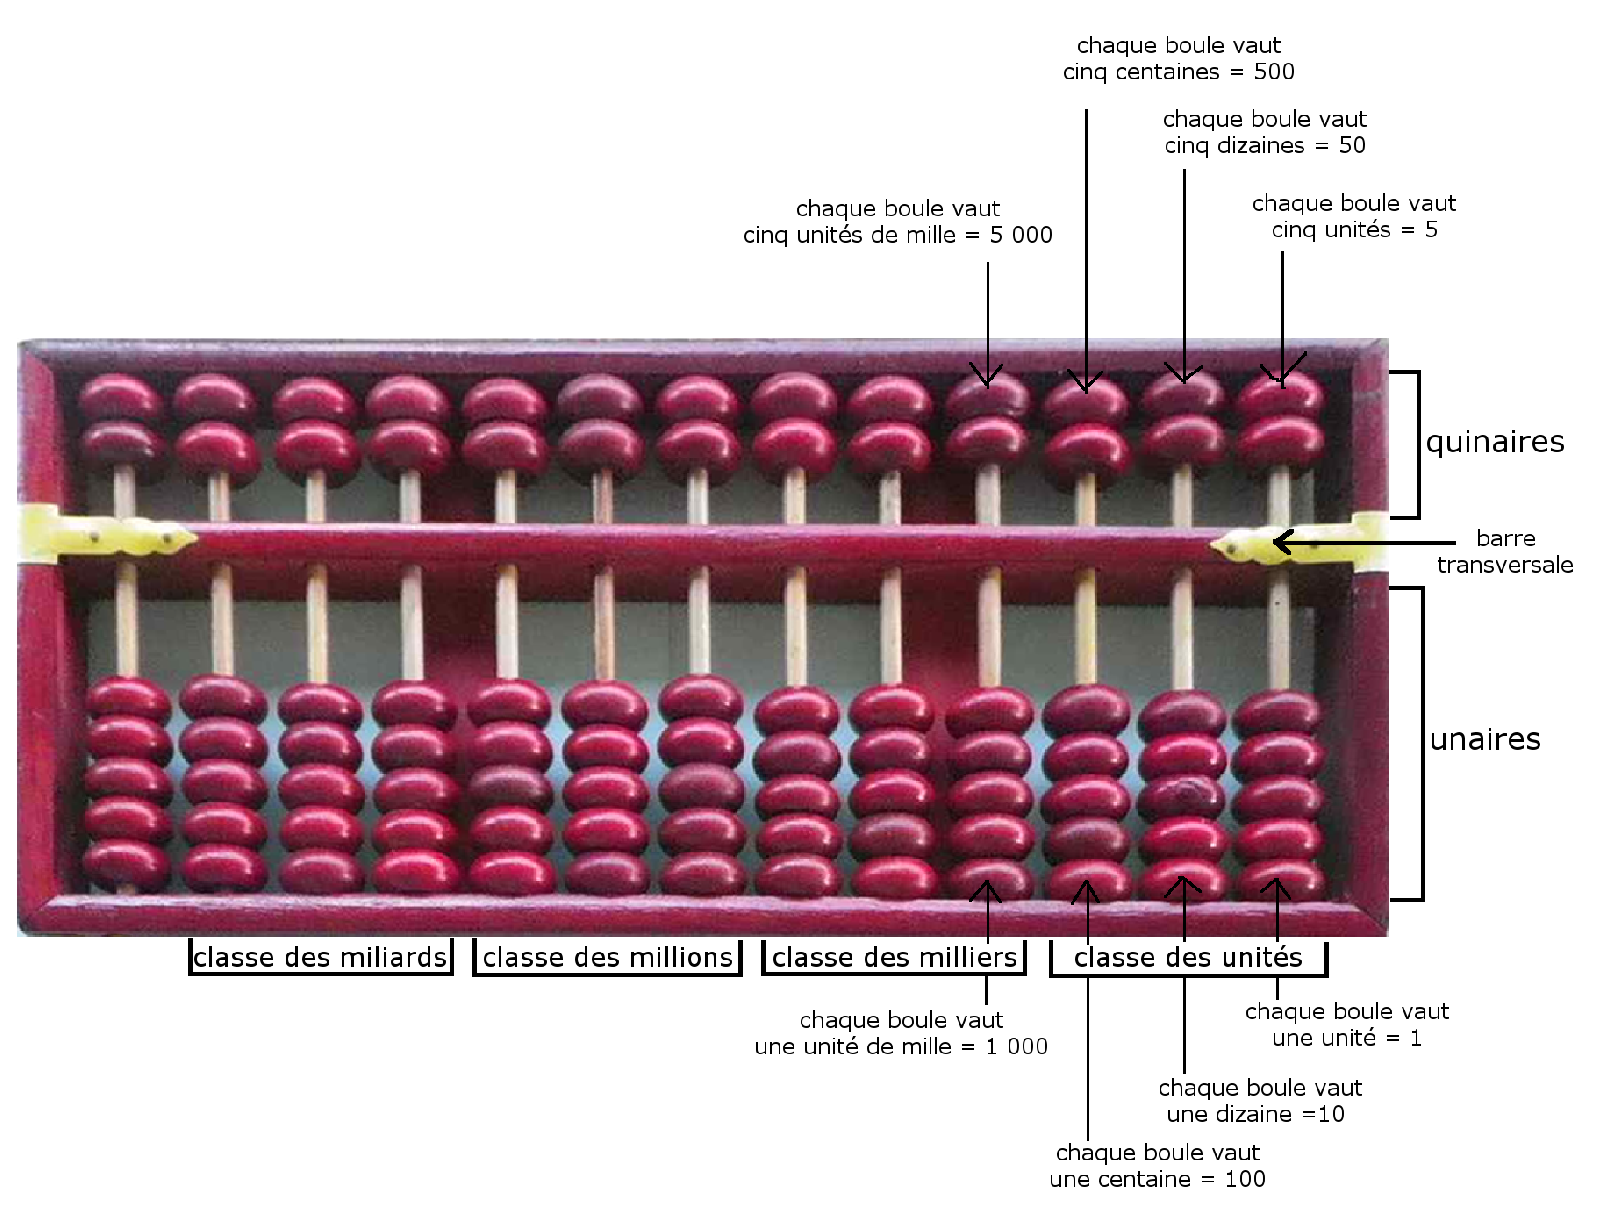
\includegraphics[width=11cm]{Nombres_et_calculs_did/Images/Num1_activites_boulier}
   \end{center}  
   \item {\bf L'abaque à jetons romain} \\
   Les colones verticales représentent les différents ordres : unités, dizaines, centaines, milliers, dizaines de milliers\dots. Pour représenter un nombre, il suffit de placer, pour chaque ordre, autant de jetons que la valeur du chiffre. Il s'apparente au traditionnel tableau de numération. \\
   \begin{center}
      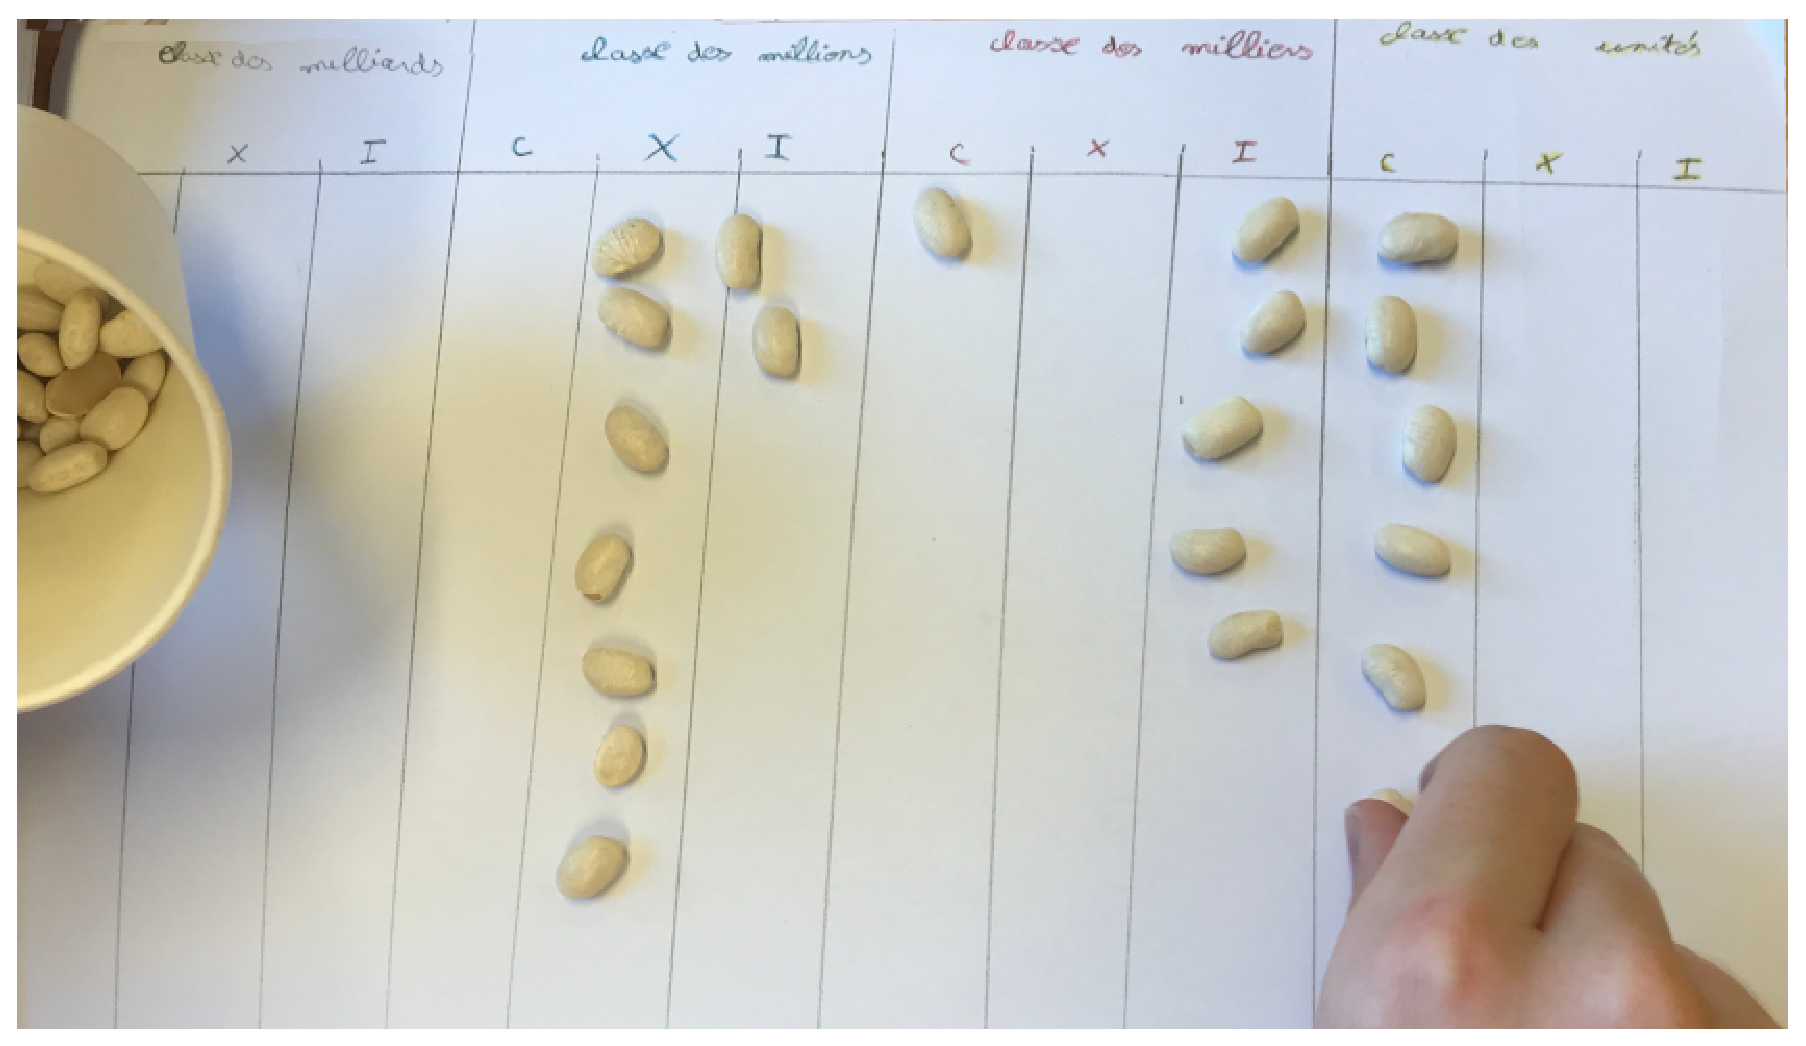
\includegraphics[width=9cm]{Nombres_et_calculs_did/Images/Num1_activites_abaque_romain}
   \end{center}    
   L'utilisation de l'un ou l'autre de ces abaques devrait se faire en fil rouge tout au long de l'année, comme outil de représentation des nombres, de vérification, de remédiation\dots{} Quand l'élève se l'ai bien approprié, on peut proposer de faire des calculs à l'abaque.
\end{enumerate}
\end{exercice*}   

